\documentclass[a4paper]{article}

\usepackage[pdftex,
            hidelinks,
            pdfauthor={Dexter Chua},
            pdfsubject={Cambridge Maths Notes: Part IA - Vectors and Matrices},
            pdftitle={Part IA - Vectors and Matrices},
            pdfkeywords={Cambridge Mathematics Maths Math IA Michaelmas Vectors and Matrices}]{hyperref}

% Imports
\ifx \nextra \undefined
  \usepackage[pdftex,
    hidelinks,
    pdfauthor={Dexter Chua},
    pdfsubject={Cambridge Maths Notes: Part \npart\ - \ncourse},
    pdftitle={Part \npart\ - \ncourse},
  pdfkeywords={Cambridge Mathematics Maths Math \npart\ \nterm\ \nyear\ \ncourse}]{hyperref}
  \title{Part \npart\ - \ncourse}
\else
  \usepackage[pdftex,
    hidelinks,
    pdfauthor={Dexter Chua},
    pdfsubject={Cambridge Maths Notes: Part \npart\ - \ncourse\ (\nextra)},
    pdftitle={Part \npart\ - \ncourse\ (\nextra)},
  pdfkeywords={Cambridge Mathematics Maths Math \npart\ \nterm\ \nyear\ \ncourse\ \nextra}]{hyperref}

  \title{Part \npart\ - \ncourse \\ {\Large \nextra}}
\fi

\author{Lectured by \nlecturer \\\small Notes taken by Dexter Chua}
\date{\nterm\ \nyear}

\usepackage{alltt}
\usepackage{amsfonts}
\usepackage{amsmath}
\usepackage{amssymb}
\usepackage{amsthm}
\usepackage{booktabs}
\usepackage{caption}
\usepackage{enumitem}
\usepackage{fancyhdr}
\usepackage{graphicx}
\usepackage{mathtools}
\usepackage{microtype}
\usepackage{multirow}
\usepackage{pdflscape}
\usepackage{pgfplots}
\usepackage{siunitx}
\usepackage{tabularx}
\usepackage{tikz}
\usepackage{tkz-euclide}
\usepackage[normalem]{ulem}
\usepackage[all]{xy}

\pgfplotsset{compat=1.12}

\pagestyle{fancyplain}
\lhead{\emph{\nouppercase{\leftmark}}}
\ifx \nextra \undefined
  \rhead{
    \ifnum\thepage=1
    \else
      \npart\ \ncourse
    \fi}
\else
  \rhead{
    \ifnum\thepage=1
    \else
      \npart\ \ncourse\ (\nextra)
    \fi}
\fi
\usetikzlibrary{arrows}
\usetikzlibrary{decorations.markings}
\usetikzlibrary{decorations.pathmorphing}
\usetikzlibrary{positioning}
\usetikzlibrary{fadings}
\usetikzlibrary{intersections}
\usetikzlibrary{cd}

\newcommand*{\Cdot}{\raisebox{-0.25ex}{\scalebox{1.5}{$\cdot$}}}
\newcommand {\pd}[2][ ]{
  \ifx #1 { }
    \frac{\partial}{\partial #2}
  \else
    \frac{\partial^{#1}}{\partial #2^{#1}}
  \fi
}

% Theorems
\theoremstyle{definition}
\newtheorem*{aim}{Aim}
\newtheorem*{axiom}{Axiom}
\newtheorem*{claim}{Claim}
\newtheorem*{cor}{Corollary}
\newtheorem*{defi}{Definition}
\newtheorem*{eg}{Example}
\newtheorem*{fact}{Fact}
\newtheorem*{law}{Law}
\newtheorem*{lemma}{Lemma}
\newtheorem*{notation}{Notation}
\newtheorem*{prop}{Proposition}
\newtheorem*{thm}{Theorem}

\renewcommand{\labelitemi}{--}
\renewcommand{\labelitemii}{$\circ$}
\renewcommand{\labelenumi}{(\roman{*})}

\let\stdsection\section
\renewcommand\section{\newpage\stdsection}

% Strike through
\def\st{\bgroup \ULdepth=-.55ex \ULset}

% Maths symbols
\newcommand{\bra}{\langle}
\newcommand{\ket}{\rangle}

\newcommand{\N}{\mathbb{N}}
\newcommand{\Z}{\mathbb{Z}}
\newcommand{\Q}{\mathbb{Q}}
\renewcommand{\H}{\mathbb{H}}
\newcommand{\R}{\mathbb{R}}
\newcommand{\C}{\mathbb{C}}
\newcommand{\Prob}{\mathbb{P}}
\renewcommand{\P}{\mathbb{P}}
\newcommand{\E}{\mathbb{E}}
\newcommand{\F}{\mathbb{F}}
\newcommand{\cU}{\mathcal{U}}
\newcommand{\RP}{\mathbb{RP}}
\newcommand{\CP}{\mathbb{CP}}

\newcommand{\ph}{\,\cdot\,}

\DeclareMathOperator{\sech}{sech}
\DeclareMathOperator{\cosech}{cosech}
\DeclareMathOperator{\cosec}{cosec}

\DeclareMathOperator{\covol}{covol}
\DeclareMathOperator{\vol}{vol}

\let\Im\relax
\let\Re\relax
\DeclareMathOperator{\Im}{Im}
\DeclareMathOperator{\Re}{Re}
\DeclareMathOperator{\im}{im}
\DeclareMathOperator{\image}{image}
\DeclareMathOperator{\Ann}{Ann}

\DeclareMathOperator*{\res}{res}
\DeclareMathOperator{\Res}{Res}
\DeclareMathOperator{\Ind}{Ind}

\DeclareMathOperator{\tr}{tr}
\DeclareMathOperator{\diag}{diag}
\DeclareMathOperator{\rank}{rank}
\DeclareMathOperator{\card}{card}
\DeclareMathOperator{\spn}{span}
\DeclareMathOperator{\adj}{adj}

\DeclareMathOperator{\erf}{erf}
\DeclareMathOperator{\erfc}{erfc}

\DeclareMathOperator{\ord}{ord}
\DeclareMathOperator{\Sym}{Sym}

\DeclareMathOperator{\sgn}{sgn}
\DeclareMathOperator{\orb}{orb}
\DeclareMathOperator{\stab}{stab}
\DeclareMathOperator{\ccl}{ccl}

\DeclareMathOperator{\lcm}{lcm}
\DeclareMathOperator{\hcf}{hcf}

\DeclareMathOperator{\Int}{Int}
\DeclareMathOperator{\id}{id}

\DeclareMathOperator{\betaD}{beta}
\DeclareMathOperator{\gammaD}{gamma}
\DeclareMathOperator{\Poisson}{Poisson}
\DeclareMathOperator{\binomial}{binomial}
\DeclareMathOperator{\multinomial}{multinomial}
\DeclareMathOperator{\Bernoulli}{Bernoulli}
\DeclareMathOperator{\like}{like}

\DeclareMathOperator{\var}{var}
\DeclareMathOperator{\cov}{cov}
\DeclareMathOperator{\bias}{bias}
\DeclareMathOperator{\mse}{mse}
\DeclareMathOperator{\corr}{corr}

\DeclareMathOperator{\otp}{otp}
\DeclareMathOperator{\dom}{dom}

\DeclareMathOperator{\Root}{Root}
\DeclareMathOperator{\supp}{supp}
\DeclareMathOperator{\rel}{rel}
\DeclareMathOperator{\Hom}{Hom}
\DeclareMathOperator{\Aut}{Aut}
\DeclareMathOperator{\Gal}{Gal}
\DeclareMathOperator{\Mat}{Mat}
\DeclareMathOperator{\End}{End}
\DeclareMathOperator{\Char}{char}
\DeclareMathOperator{\ev}{ev}
\DeclareMathOperator{\St}{St}
\DeclareMathOperator{\Lk}{Lk}
\DeclareMathOperator{\disc}{disc}
\DeclareMathOperator{\Isom}{Isom}
\DeclareMathOperator{\length}{length}
\DeclareMathOperator{\energy}{energy}
\DeclareMathOperator{\area}{area}
\DeclareMathOperator{\Syl}{Syl}
\DeclareMathOperator{\cl}{cl}
\DeclareMathOperator{\fix}{fix}

\newcommand{\GL}{\mathrm{GL}}
\newcommand{\SL}{\mathrm{SL}}
\newcommand{\PGL}{\mathrm{PGL}}
\newcommand{\PSL}{\mathrm{PSL}}
\newcommand{\PSU}{\mathrm{PSU}}
\newcommand{\Or}{\mathrm{O}}
\newcommand{\SO}{\mathrm{SO}}
\newcommand{\U}{\mathrm{U}}
\newcommand{\SU}{\mathrm{SU}}

\renewcommand{\d}{\mathrm{d}}
\newcommand{\D}{\mathrm{D}}

\tikzset{->/.style = {decoration={markings,
                                  mark=at position 1 with {\arrow[scale=2]{latex'}}},
                      postaction={decorate}}}
\tikzset{<-/.style = {decoration={markings,
                                  mark=at position 0 with {\arrowreversed[scale=2]{latex'}}},
                      postaction={decorate}}}
\tikzset{<->/.style = {decoration={markings,
                                   mark=at position 0 with {\arrowreversed[scale=2]{latex'}},
                                   mark=at position 1 with {\arrow[scale=2]{latex'}}},
                       postaction={decorate}}}
\tikzset{->-/.style = {decoration={markings,
                                   mark=at position #1 with {\arrow[scale=2]{latex'}}},
                       postaction={decorate}}}
\tikzset{-<-/.style = {decoration={markings,
                                   mark=at position #1 with {\arrowreversed[scale=2]{latex'}}},
                       postaction={decorate}}}

\tikzset{circ/.style = {fill, circle, inner sep = 0, minimum size = 3}}
\tikzset{mstate/.style={circle, draw, blue, text=black, minimum width=0.7cm}}

\definecolor{mblue}{rgb}{0.2, 0.3, 0.8}
\definecolor{morange}{rgb}{1, 0.5, 0}
\definecolor{mgreen}{rgb}{0.1, 0.4, 0.2}
\definecolor{mred}{rgb}{0.5, 0, 0}

\def\drawcirculararc(#1,#2)(#3,#4)(#5,#6){%
    \pgfmathsetmacro\cA{(#1*#1+#2*#2-#3*#3-#4*#4)/2}%
    \pgfmathsetmacro\cB{(#1*#1+#2*#2-#5*#5-#6*#6)/2}%
    \pgfmathsetmacro\cy{(\cB*(#1-#3)-\cA*(#1-#5))/%
                        ((#2-#6)*(#1-#3)-(#2-#4)*(#1-#5))}%
    \pgfmathsetmacro\cx{(\cA-\cy*(#2-#4))/(#1-#3)}%
    \pgfmathsetmacro\cr{sqrt((#1-\cx)*(#1-\cx)+(#2-\cy)*(#2-\cy))}%
    \pgfmathsetmacro\cA{atan2(#2-\cy,#1-\cx)}%
    \pgfmathsetmacro\cB{atan2(#6-\cy,#5-\cx)}%
    \pgfmathparse{\cB<\cA}%
    \ifnum\pgfmathresult=1
        \pgfmathsetmacro\cB{\cB+360}%
    \fi
    \draw (#1,#2) arc (\cA:\cB:\cr);%
}
\newcommand\getCoord[3]{\newdimen{#1}\newdimen{#2}\pgfextractx{#1}{\pgfpointanchor{#3}{center}}\pgfextracty{#2}{\pgfpointanchor{#3}{center}}}

\def\Xint#1{\mathchoice
   {\XXint\displaystyle\textstyle{#1}}%
   {\XXint\textstyle\scriptstyle{#1}}%
   {\XXint\scriptstyle\scriptscriptstyle{#1}}%
   {\XXint\scriptscriptstyle\scriptscriptstyle{#1}}%
   \!\int}
\def\XXint#1#2#3{{\setbox0=\hbox{$#1{#2#3}{\int}$}
     \vcenter{\hbox{$#2#3$}}\kern-.5\wd0}}
\def\ddashint{\Xint=}
\def\dashint{\Xint-}


\title{Part IA - Vectors and Matrices}
\author{Lectured by N. Peake}
\date{Michaelmas 2014}

\begin{document}
\maketitle
{\small \noindent\textbf{Complex numbers}\\
Review of complex numbers, including complex conjugate, inverse, modulus, argument and Argand diagram. Informal treatment of complex logarithm, $n$-th roots and complex powers. de Moivre's theorem.\hspace*{\fill}[2]

\vspace{10pt}
\noindent\textbf{Vectors}\\
Review of elementary algebra of vectors in $\R^3$, including scalar product. Brief discussion of vectors in $\R^n$ and $\C^n$; scalar product and the Cauchy–Schwarz inequality. Concepts of linear span, linear independence, subspaces, basis and dimension.

\vspace{5pt}
\noindent Suffix notation: including summation convention, $\delta_{ij}$ and $\epsilon_{ijk}$. Vector product and triple product: definition and geometrical interpretation. Solution of linear vector equations. Applications of vectors to geometry, including equations of lines, planes and spheres.\hspace*{\fill}[5]

\vspace{10pt}
\noindent\textbf{Matrices}\\
Elementary algebra of $3\times 3$ matrices, including determinants. Extension to $n\times n$ complex matrices. Trace, determinant, non-singular matrices and inverses. Matrices as linear transformations; examples of geometrical actions including rotations, reflections, dilations, shears; kernel and image.\hspace*{\fill}[4]

\vspace{5pt}
\noindent Simultaneous linear equations: matrix formulation; existence and uniqueness of solutions, geometric interpretation; Gaussian elimination.\hspace*{\fill}[3]

\vspace{5pt}
\noindent Symmetric, anti-symmetric, orthogonal, hermitian and unitary matrices. Decomposition of a general matrix into isotropic, symmetric trace-free and antisymmetric parts.\hspace*{\fill}[1]

\vspace{10pt}
\noindent\textbf{Eigenvalues and Eigenvectors}\\
Eigenvalues and eigenvectors; geometric significance.\hspace*{\fill}[2]

\vspace{5pt}
\noindent Proof that eigenvalues of hermitian matrix are real, and that distinct eigenvalues give an orthogonal basis of eigenvectors. The effect of a general change of basis (similarity transformations). Diagonalization of general matrices: sufficient conditions; examples of matrices that cannot be diagonalized. Canonical forms for $2 \times 2$ matrices.\hspace*{\fill}[5]

\vspace{5pt}
\noindent Discussion of quadratic forms, including change of basis. Classification of conics, cartesian and polar forms.\hspace*{\fill}[1]

\vspace{5pt}
\noindent Rotation matrices and Lorentz transformations as transformation groups.\hspace*{\fill}[1]}

\tableofcontents

\section{Complex numbers}
\subsection{Basic properties}
\begin{defi}[Complex number]
  A \emph{complex number} is a number $z\in \C$ of the form $z = a + ib$ with $a, b\in \R$, where $i^2=-1$. We write $a = \re(z)$ and $b = \im(z)$.
\end{defi}

We have
\begin{align*}
  z_1\pm z_2 &= (a_1 + ib_1)\pm (a_2 + ib_2)\\
  &= (a_1\pm a_2) + (b_1 \pm b_2)\\
  z_1z_2 &= (a_1 + ib_1)(a_2 + ib_2)\\
  &= (a_1a_2 - b_1b_2) + i(b_1a_2 + a_1b_2)\\
  z^{-1} &= \frac{1}{a + ib}\\
  &= \frac{a - ib}{a^2 + b^2}
\end{align*}
\begin{defi}[Complex conjugate]
  The \emph{complex conjugate} of $z = a+ ib$ is $\bar{z} = z^* = a - ib$.
\end{defi}

\begin{defi}[Argand diagram]
  An \emph{Argand diagram} is a diagram in which a complex number $z = x + iy$ is represented by a vector $\mb{p}=\begin{pmatrix}x\\y\end{pmatrix}$. Addition of vectors corresponds to vector addition and $\bar{z}$ is the reflection of $z$ in the $x$-axis.
\end{defi}

\begin{center}
  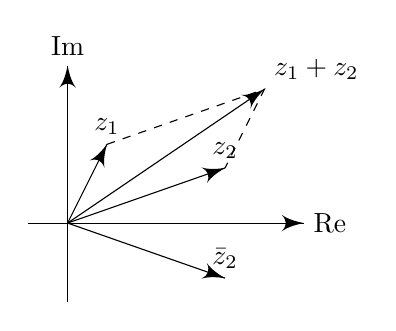
\begin{tikzpicture}
    \draw [->] (-0.5, 0) -- (3, 0) node [right] {Re};
    \draw [->] (0, -1) -- (0, 2) node [above] {Im};
    \draw [->] (0, 0) -- (.5, 1) node [above] {$z_1$};
    \draw [->] (0, 0) -- (2, .7) node [above] {$z_2$};
    \draw [->] (0, 0) -- (2, -.7) node [above] {$\bar z_2$};
    \draw [->] (0, 0) -- (2.5, 1.7) node [anchor=south west] {$z_1 + z_2$};
    \draw [dashed] (.5, 1) -- (2.5, 1.7) -- (2, .7);
  \end{tikzpicture}
\end{center}

\begin{defi}[Modulus and argument of complex number]
  The \emph{modulus} of $z = x + iy$ is $r = |z| = \sqrt{x^2 + y^2}$. The \emph{argument} is $\theta = \arg z = \tan^{-1} (y/x)$. The modulus is the length of the vector in the Argand diagram, and the argument is the angle between $z$ and the real axis. We have
  \[
  z = r(\cos\theta + i\sin \theta)
  \]

  Clearly the pair $(r, \theta)$ uniquely describes a complex number $z$, but each complex number $z\in \C$ can be described by many different $\theta$ since $\sin (2\pi + \theta) = \sin \theta$ and $\cos(2\pi + \theta) = \cos\theta$. Often we take the \emph{principle value} $-\pi < \theta \leq \pi$.
\end{defi}

When writing $z_i = r_i(\cos\theta_i + i\sin \theta_i)$, we have
\begin{align*}
  z_1z_2 &= r_1r_2[(\cos\theta_1\cos\theta_2 - \sin\theta_1\sin\theta_2) + i(\sin\theta_1\cos\theta_2 + \sin\theta_2\cos\theta_1)]\\
  &= r_1r_2[\cos(\theta_1 + \theta_2) + i\sin(\theta_1+\theta_2)]
\end{align*}
i.e. moduli multiply and arguments add.

\begin{prop}
  $z\bar{z} = a^2 + b^2 = |z|^2$.
\end{prop}

\begin{prop}
  $z^{-1} = \bar{z}/|z|^2$.
\end{prop}

\begin{thm}[Triangle inequality]
  For all $z_1, z_2 \in \C$, we have
  \[
  |z_1 + z_2| \leq |z_1| + |z_2|.
  \]
  Alternatively, we have $|z_1 - z_2|\geq ||z_1| - |z_2||$.
\end{thm}

\subsection{Complex exponential function}
\begin{defi}[Exponential function]
  The \emph{exponential function} is defined as
  \[
  \exp (z) = 1 + z + \frac{z^2}{2!} + \frac{z^3}{3!} + \cdots = \sum_{n = 0}^\infty \frac{z^n}{n!}.
  \]
\end{defi}

\begin{lemma}
  \[
  \sum_{n = 0}^\infty\sum_{m = 0}^\infty a_{mn} = \sum_{r = 0}^\infty\sum_{m = 0}^r a_{r - m, m}
  \]
\end{lemma}

\begin{proof}
  \begin{align*}
    \sum_{n = 0}^\infty\sum_{m = 0}^\infty a_{mn} &= a_{00} + a_{01} + a_{02} + \cdots\\
    &+ a_{10} + a_{11} + a_{12} + \cdots\\
    &+ a_{20} + a_{21} + a_{22} + \cdots\\
    &= (a_{00}) + (a_{10} + a_{01}) + (a_{20} + a_{11} + a_{02}) + \cdots\\
    &= \sum_{r = 0}^\infty\sum_{m = 0}^r a_{r - m, m}
  \end{align*}
\end{proof}
\begin{thm}
  $\exp(z_1)\exp(z_2) = \exp(z_1 + z_2)$
\end{thm}

\begin{proof}
  \begin{align*}
    \exp(z_1)\exp(z_2) &= \sum_{n = 0}^\infty\sum_{m = 0}^\infty \frac{z_1^m}{m!}\frac{z_2^n}{n!}\\
    &= \sum_{r = 0}^\infty\sum_{m = 0}^r \frac{z_1^{r - m}}{(r - m)!}\frac{z_2^m}{m!}\\
    &= \sum_{r = 0}^\infty\frac{1}{r!}\sum_{m = 0}^r \frac{r!}{(r - m)!m!}z_1^{r - m}z_2^m\\
    &= \sum_{r = 0}^\infty\frac{(z_1 + z_2)^r}{r!}
  \end{align*}
\end{proof}

\begin{defi}[Sine and cosine functions]
  Define, for all $z\in \C$,
  \begin{alignat*}{2}
    \sin z &= \sum_{n=0}^\infty \frac{(-1)^n}{(2n+1)!}z^{2n+1} &\;= z - \frac{1}{3!}z^3 + \frac{1}{5!}z^5 + \cdots\\
    \cos z &= \sum_{n=0}^\infty \frac{(-1)^n}{(2n)!}z^{2n} &\;= 1 - \frac{1}{2!}z^2 + \frac{1}{4!}z^4 + \cdots
  \end{alignat*}
\end{defi}

\begin{thm}
  $e^{iz} = \cos z + i\sin z$
\end{thm}

\begin{proof}
  \begin{align*}
  e^{iz} &= \sum_{n=0}^\infty \frac{i^n}{n!}z^n\\
  &= \sum_{n=0}^\infty \frac{i^{2n}}{(2n)!}z^{2n} + \sum_{n=0}^\infty \frac{i^{2n+1}}{(2n+1)!}z^{2n+1}\\
  &= \sum_{n=0}^\infty \frac{(-1)^n}{(2n)!}z^{2n} + i \sum_{n=0}^\infty \frac{(-1)^n}{(2n+1)!}z^{2n+1}\\
  &= \cos z + i\sin z
  \end{align*}
\end{proof}
Thus we can write $z = r(\cos\theta + i\sin\theta) = re^{i\theta}$.

\subsection{Roots of unity}
\begin{defi}[Roots of unity]
  The $n$-th \emph{roots of unity} are the roots to the solution $z^n = 1$ for $n\in \N$. Since this is a polynomial of order $n$, there are $n$ roots of unity. The $n$-th roots of unity are $\exp\left(2\pi i\frac{k}{n}\right)$ for $k = 0, 1, 2, 3\cdots n - 1$.
\end{defi}

\begin{prop}
  If $\omega = \exp\left(\frac{2\pi i}{n}\right)$, then $1 + \omega + \omega^2 + \cdots + \omega^{n - 1} = 1$
\end{prop}

\begin{proof}
  Two proofs are provided:
  \begin{enumerate}
  \item Consider the equation $z^n = 1$. The coefficient of $z^{n-1}$ is the sum of all roots. Since the coefficient of $z^{n-1}$ is 0, then the sum of all roots $= 1 + \omega + \omega^2 + \cdots + \omega^{n-1} = 0$.
  \item Since $\omega^n - 1 = (\omega - 1)(1 + \omega + \cdots + \omega^{n - 1})$ and $\omega \not= 1$, dividing by $(\omega - 1)$, we have $1 + \omega + \cdots + \omega^{n-1} = (\omega^n - 1)/(\omega - 1) = 0$.
  \end{enumerate}
\end{proof}

\subsection{Complex logarithm and power}
\begin{defi}[Complex logarithm]
  The \emph{complex logarithm} $\log z$ is a solution to $e^\omega = z$. i.e. $\omega = \log z$. Writing $z = re^{i\theta}$, we have $\log z = \log(re^{i\theta}) = \log r + i\theta$. This can multi-valued for different values of $\theta$ and, as above, we should select the $\theta$ that satisfies $-\pi < \theta \leq \pi$.
\end{defi}
\begin{eg}
  $\log 2i = \log 2 + i\frac{\pi}{2}$
\end{eg}

\begin{defi}[Complex power]
  The \emph{complex power} $z^\alpha$ for $z, \alpha\in \C$ is defined as $z^\alpha = e^{\alpha\log z}$. This complex power can be multi-valued, as $z^\alpha = e^{\alpha\log|z|}e^{i\alpha\theta}e^{2in\pi\alpha}$ (there are finitely many values if $\alpha\in\Q$, infinitely many otherwise). Nevertheless, make $z^\alpha$ single-valued by insisting $-\pi < \theta \leq \pi$.
\end{defi}

\subsection{De Moivre's theorem}
\begin{thm}[De Moivre's theorem]
\[
\cos n\theta + i\sin n\theta = (\cos\theta + i\sin\theta)^n.
\]
\end{thm}
\begin{proof}
  First prove for the $n \geq 0$ case by induction. The $n = 0$ case is true since it merely reads $1 = 1$. We then have
  \begin{align*}
    (\cos\theta + i\sin\theta)^{n + 1} &= (\cos\theta + i\sin\theta)^n (\cos\theta + i\sin\theta)\\
    &= (\cos n\theta + i\sin n\theta )(\cos\theta + i\sin\theta)\\
    &= \cos(n+1)\theta + \sin(n+1)\theta
  \end{align*}
  If $n < 0$, let $m = -n$. Then $m > 0$ and
  \begin{align*}
    (cos\theta + i\sin\theta)^{-m} &= (\cos m\theta + i\sin m\theta)^{-1}\\
    &= \frac{\cos m\theta - i\sin m\theta}{(\cos m\theta + i\sin m\theta)(\cos m\theta - i\sin m\theta)}\\
    &= \frac{\cos (-m\theta) + i\sin (-m\theta)}{\cos^2 m\theta + \sin^2 m\theta}\\
    &= \cos (-m\theta) + i\sin (-m\theta)\\
    &= \cos n\theta + i\sin n\theta
  \end{align*}
\end{proof}

\begin{eg}
  We have $\cos 5\theta + i\sin5\theta  = (\cos\theta + i\sin\theta)^5$. By binomial expansion of the RHS and taking real and imaginary parts, we have
  \begin{align*}
    \cos 5\theta &= 5\cos\theta - 20\cos^3\theta + 16\cos^5\theta\\
    \sin 5\theta &= 5\sin\theta - 20\sin^3\theta + 16\sin^5\theta
  \end{align*}
\end{eg}

\subsection{Lines and circles in \texorpdfstring{$\C$}{C}}
\begin{thm}
The general equation of a straight line through $z_0\in \C$ parallel to $w\in \C$ can be given by $z = z_0 + \lambda w$ for $\lambda \in \R$. This can be rearranged to $\lambda = \frac{z - z_0}{w}$. Taking the complex conjugate, we have $\bar{\lambda} = \frac{\bar{z} - \bar{z_0}}{\bar{w}}$. However, since $\lambda$ is real, we have $\lambda = \bar{\lambda}$. Thus we have
\begin{align*}
  \frac{z - z_0}{w} &= \frac{\bar{z} - \bar{z_0}}{\bar{w}}\\
  z\bar w - \bar z w &= z_0 \bar w - \bar z_0 w
\end{align*}

The general equation of a circle with center $c\in \C$ and radius $\rho \in \R^+$ can be given by
\begin{align*}
  |z - c| &= \rho\\
  |z - c|^2 &= \rho^2\\
  (z - c)(\bar z - \bar c) &= \rho^2\\
  z\bar z - \bar c z - c\bar z &= \rho^2 - c\bar c
\end{align*}
\end{thm}
\section{Vectors}
\subsection{Definition and basic properties}

\begin{defi}[Vector]
  A \emph{vector} $\mb{v}$ has a (positive) length and direction.  If $|\mb{v}| = 0$, then $\mb{v} = \mb{0}$.

  Vectors can be added together or multiplied by a scalar in $\R$ or $\C$. Vector addition satisfies the following axioms:
  \begin{enumerate}
  \item (Commutativity) $\mb{a} + \mb{b} = \mb{b} + \mb{a}$
  \item (Associativity) $(\mb{a} + \mb{b}) + \mb{c} = \mb{a} + (\mb{b} + \mb{c})$
  \item (Identity) There is a vector $\mb{0}$ such that $\mb{a} + \mb{0} = \mb{a}$.
  \item (Inverse) For all vectors $\mb{a}$, there is a vector $(-\mb{a})$ such that $\mb{a} + (-\mb{a}) = \mb{0}$.
  \end{enumerate}
  \emph{Scalar multiplication} satisfies the following axioms:
  \begin{enumerate}
  \item $\lambda\mb{a}$ is either parallel ($\lambda > 0$) to or anti-parallel ($\lambda < 0$) to $\mb{a}$.
  \item $\lambda(\mb{a + b}) = \lambda\mb{a} + \lambda\mb{b}$.
  \item $(\lambda + \mu)\mb{a} = \lambda\mb{a} + \mu\mb{a}$.
  \item $\lambda(\mu\mb{a}) = \mu(\lambda\mb{a}) = (\mu\lambda)\mb{a}$.
  \item $1\mb{a = a}$.
  \end{enumerate}
\end{defi}

\begin{defi}[Unit vector]
  A \emph{unit vector} is a vector with length 1. We write a unit vector as $\hat{\mb{v}}$.
\end{defi}

\begin{eg}
  $\R^n$ is a vector space with component-wise addition and scalar multiplication. Note that vector space $\R$ is a line, but not all lines are vector spaces. e.g. $x + y = 1$ is not a vector space since it does not contain $\mb{0}$.
\end{eg}

\subsection{Scalar product}
\subsubsection{Geometric picture (\texorpdfstring{$\R^2$}{R2} and \texorpdfstring{$\R^3$}{R3} only)}
\begin{defi}[Scalar/dot product]
  $\mb{a}\cdot\mb{b} = \mb{|a||b|}\cos\theta$, where $\theta$ is the angle between $\mb{a}$ and $\mb{b}$. It satisfies the following properties:
  \begin{enumerate}
  \item $\mb{a\cdot b = b\cdot a}$
  \item $\mb{a\cdot a = |a|}^2 \geq 0$
  \item $\mb{a\cdot a} = 0$ iff $\mb{a = 0}$
  \item If $\mb{a\cdot b} = 0$ and $\mb{a, b}\not= 0$, then $\mb{a \perp b}$.
  \end{enumerate}
\end{defi}

The projection of $\mb{b}$ onto $\mb{a}$ is given by $(|\mb{b}|\cos\theta)\hat{\mb{a}} = \mb{(\hat{a}\cdot b)\hat{a}}$

The cosine rule can be derived as follows:
\begin{align*}
  |\overrightarrow{BC}|^2 &= |\overrightarrow{AB} + \overrightarrow{AC}|^2\\
  &= (\overrightarrow{AB} + \overrightarrow{AC})(\overrightarrow{AB} + \overrightarrow{AC})\\
  &= |\overrightarrow{AB}|^2 + |\overrightarrow{AC}|^2 - 2|\overrightarrow{AB}||\overrightarrow{AC}|\cos\theta
\end{align*}

\subsubsection{General algebraic definition}
\begin{defi}[Inner/scalar product]
  In a real vector space $V$, the \emph{inner product} or \emph{scalar product} is a map $V\times V\to \R$ that satisfies the following axioms. It is written as $\mb{x\cdot y}$ or $\bra\mb{x|y}\ket$ (Dirac bra-ket notation).
  \begin{enumerate}
  \item (Symmetry) $\mb{x\cdot y = y\cdot x}$
  \item (Linearity in 2nd argument) $\mb{x}\cdot (\lambda\mb{y} + \mu\mb{z}) = \lambda\mb{x\cdot y} + \mu\mb{x\cdot z}$
  \item (Positive definite) $\mb{x\cdot x}\geq 0$ with equality iff $\mb{x = 0}$.
  \end{enumerate}
\end{defi}
\note (i) and (ii) together can be used to show linearity in 1st argument, but only for real numbers.

\begin{defi}
  The \emph{norm} of a vector, written as $|\mb{a}|$ or $||\mb{a}||$, is defined as
  \[
  |\mb{a}| = \sqrt{\mb{a\cdot a}}
  \]
\end{defi}

\begin{eg}
  The following is an inner product of 2 real functions $f$ and $g$ on $[0, 1]$:
  \[
  \bra f|g\ket = \int_0^1f(x)g(x)\;\mathrm{d} x
  \]
\end{eg}

\subsection{Cauchy-Schwarz inequality}
\begin{thm}[Cauchy-Schwarz inequality]
  For all $\mb{x, y}\in \R$,
  \[
  \mb{x\cdot y \leq |x||y|}
  \]
\end{thm}

\begin{proof}
  \begin{align*}
    |\mb{x} - \lambda\mb{y}|^2 \geq 0\\
    (\lambda{x} - \lambda\mb{y})(\lambda{x} - \lambda\mb{y}) \geq 0\\
    \lambda^2 |\mb{y}|^2 - \lambda (2\mb{x\cdot y}) + |\mb{x}|^2 \geq 0
  \end{align*}
  Viewing this as a quadratic in $\lambda$, we see that the quadratic is non-negative and thus cannot have 2 real roots. Thus the determinant $\Delta \leq 0$
  \begin{align*}
    4(\mb{x\cdot y})^2 &\leq 4|\mb{y}|^2|\mb{x}|^2\\
    (\mb{x\cdot y})^2 &\leq |\mb{x}|^2|\mb{y}|^2\\
    \mb{x\cdot y} &\leq \mb{|x||y|}
  \end{align*}
\end{proof}

\begin{eg}
  Let $\mb{x} = (\alpha, \beta, \gamma)$ and $\mb{y} = (1, 1, 1)$. Then by the Cauchy-Schwarz inequality, we have
  \begin{align*}
    \alpha + \beta + \gamma &\leq \sqrt{3}\sqrt{\alpha^2 + \beta^2 + \gamma^2}\\
    \alpha^2 + \beta^2 + \gamma^2 &\geq \alpha\beta + \beta\gamma + \gamma\alpha
  \end{align*}
  With equality if $\alpha = \beta = \gamma$.
\end{eg}

\begin{cor}[Triangle inequality]
  \[
  \mb{|x + y|} \leq \mb{|x| + |y|}
  \]
\end{cor}
\begin{proof}
  \begin{align*}
    |\mb{x + y}|^2 &= \mb{(x + y)\cdot (x + y)}\\
    &= |\mb{x}|^2 + 2\mb{x\cdot y} + |\mb{y}|^2\\
    &\leq |\mb{x}|^2 + 2\mb{|x||y|} + |\mb{y}|^2\\
    &= (\mb{|x| + |y|})^2\\
    \mb{|x + y|} &\leq \mb{|x| + |y|}
  \end{align*}
\end{proof}

\subsection{Vector product}
\begin{defi}[Vector/cross product]
  Consider $\mb{a, b}\in \R^3$. Define the \emph{vector product}
  \[
  \mb{a\times b} = \mb{|a||b|}\sin\theta \hat{\mb{n}},
  \]
  where $\mb{\hat{n}\perp a, b}$ in a right-handed sense. The vector product satisfies the following properties:
  \begin{enumerate}
  \item $\mb{a\times b = -b\times a}$.
  \item $\mb{a\times a = 0}$.
  \item $\mb{a\times b = 0}\Rightarrow \mb{a} = \lambda\mb{b}$ for some $\lambda\in \R$.
  \item $\mb{a}\times (\lambda \mb{b}) = \lambda(\mb{a\times b})$.
  \item $\mb{a\times (b + c) = a\times b + a\times c}$.
  \end{enumerate}
\end{defi}

The area of a triangle $OAB$ is given by $\frac{1}{2}|\overrightarrow{OA}||\overrightarrow{OB}|\sin\theta = \frac{1}{2}|\overrightarrow{OA}\times\overrightarrow{OB}|$. Define the vector area as $\frac{1}{2}\overrightarrow{OA}\times\overrightarrow{OB}$.

\subsection{Scalar triple product}
\begin{defi}[Scalar triple product]
  The \emph{scalar triple product} is defined as
  \[
  \mb{[a, b, c] = a\cdot (b\times c)}.
  \]
\end{defi}

\begin{prop}
  If a parallelopiped has sides represented by vectors $\mb{a, b, c}$ that form a right-handed system, then the volume of the parallelopiped is given by $\mb{[a, b, c]}$.
\end{prop}

\begin{proof}
  The area of the base of the parallelopiped is given by $\mb{|b||c|}\sin\theta = \mb{|b\times c|}$. Thus the volume$ = \mb{|b\times c||a|}\cos\phi = \mb{|a\cdot(b\times c)|}$, where $\phi$ is the angle between $\mb{a}$ and the normal to $\mb{b}$ and $\mb{c}$. However, since $\mb{a, b, c}$ form a right-handed system, we have $\mb{a\cdot (b\times c)} \geq 0$. Therefore the volume is $\mb{a\cdot(b\times c)}$.
\end{proof}
\note The order of $\mb{a, b, c}$ doesn't affect the volume. Thus
\[
\mb{[a, b, c] = [b, c, a] = [c, a, b] = -[b, a, c] = -[a, c, b] = -[c, b, a]}.
\]

\begin{thm}
  $\mb{a\times (b + c) = a\times b + a\times c}$.
\end{thm}
\begin{proof}
  Let $\mb{d = a\times (b + c) - a\times b - a\times c}$. We have
  \begin{align*}
    \mb{d\cdot d} &= \mb{d\cdot[a\times (b + c)] - d\cdot(a\times b) - d\cdot(a\times c)}\\
    &= \mb{(b+c)\cdot(d \times a) - b\cdot(d\times a) - c\cdot(d\times a)}\\
    &= \mb{0}
  \end{align*}
  Thus $\mb{d = 0}$.
\end{proof}

\subsection{Spanning sets and bases}
\subsubsection{2D space}
\begin{defi}[Spanning set]
  A set of vectors $\{\mb{a, b}\}$ \emph{spans} $\R^2$ if for all vectors $\mb{r}\in \R^2$, there exists some $\lambda, \mu\in \R$ such that $\mb{r} = \lambda\mb{a} + \mu\mb{b}$. Two vectors span $\R^2$ if $\mb{a\times b}\not= 0$.
\end{defi}
\begin{thm}
  The coefficients $\lambda, \mu$ are unique.
\end{thm}

\begin{proof}
  Suppose that $\mb{r} = \lambda\mb{a} + \mu\mb{b} = \lambda'\mb{a} + \mu'\mb{b}$. Take the vector product with $\mb{a}$ on both sides to get $(\mu - \mu')\mb{a\times b} = 0$. Since $\mb{a\times b}\not= 0$, then $\mu=\mu'$. Similarly, $\lambda = \lambda'$.
\end{proof}

\begin{defi}[Linearly independent vectors in $\R^2$]
  Two vectors $\mb{a}$ and $\mb{b}$ are \emph{linearly independent} if  for $\alpha, \beta\in \R$, $\alpha\mb{a} + \beta\mb{b}$ iff $\alpha = \beta = 0$. In $\R^2$, $\mb{a}$ and $\mb{b}$ are linearly independent if $\mb{a\times b} \not= 0$.
\end{defi}

\begin{defi}[Basis of $\R^2$]
  A set of vectors is a \emph{basis} of $\R^2$ if it spans $\R^2$ and are linearly independent.
\end{defi}

\begin{eg}
  $\mb{\{\hat{i}, \hat{j}\}}$ is a basis of $\R^2$. They are the standard basis of $\R^2$.
\end{eg}

\subsubsection{3D space}
\begin{thm}
  If $\mb{a, b, c}\in\R^3$ are non-coplanar, i.e. $\mb{a\cdot(b\times c)}\not= 0$, then they form a basis of $\R^3$.
\end{thm}

\begin{proof}
  For any $\mb{r}$, write $\mb{r} = \lambda\mb{a} + \mu\mb{b} + \nu\mb{c}$. Performing the scalar product with $\mb{b\times c}$ on both sides, one obtains $\mb{r\cdot(b\times c)} = \lambda \mb{a\cdot(b\times c)} + \mu\mb{b\cdot (b\times c)} + \nu\mb{c\cdot(b\times c)} = \lambda \mb{[a, b, c]}$. Thus $\lambda = \mb{[r, b, c]/[a,b, c]}$. The values of $\mu$ and $\nu$ can be found similarly. Thus each $\mb{r}$ can be written as a linear combination of $\mb{a, b}$ and $\mb{c}$.

\note The above proof is not question-begging by assuming $\mb{a, b, c}$ is a basis. We can re-write it to say ``Let $\lambda = \mb{[r, b, c]/[a,b, c]}$ etc. Then $\mb{r} = \lambda\mb{a} + \mu\mb{b} + \nu\mb{c}$.'' The first line of the proof is intended to show where these magic coefficients come from, and not part of the proof proper.

By the formula derived above, it follows that if $\alpha\mb{a} + \beta\mb{b} + \gamma\mb{c} = \mb{0}$, then $\alpha = \beta = \gamma = 0$. Thus they are linearly independent.
\end{proof}

In $\R^3$, the standard basis is $\mb{\hat{i}, \hat{j}, \hat{k}}$, or $(1, 0, 0), (0, 1, 0)$ and $(0, 0, 1)$.
\subsubsection{\texorpdfstring{$\R^n$}{Rn} space}
\begin{defi}[Linearly independent vectors]
  A set of vectors $\{\mb{v}_1, \mb{v}_2, \mb{v}_3\cdots \mb{v}_m\}$ are \emph{linearly independent} if
\[
\sum_{i = 1}^m\lambda_i\mb{v}_i = \mb{0} \Rightarrow \forall i(\lambda_i = 0).
\]
\end{defi}
\begin{defi}[Spanning set]
  A set of vectors $\{\mb{u}_1, \mb{u}_2, \mb{u}_3\cdots \mb{u}_m\}\subseteq \R^n$ is a \emph{spanning set} of $\R^n$ if
  \[
  \forall \mb{x} \in \R^n\left(\exists \lambda_i\left(\sum_{i = 1}^m\lambda_i\mb{u}_i = \mb{x}\right)\right)
  \]
\end{defi}

\begin{defi}[Basis vectors]
  A \emph{basis} of $\R^n$ is a linearly independent spanning set. The standard basis of $\R^n$ is $\mb{e}_1 = (1, 0, 0, \cdots 0), \mb{e}_2 = (0, 1, 0, \cdots 0)\cdots \mb{e}_n = (0, 0, 0, \cdots, 1)$.
\end{defi}

\begin{defi}[Orthonormal basis]
  A basis $\{\mb{e}_i\}$ is \emph{orthonormal} if $\mb{e}_i\cdot \mb{e}_j = 0$ if $i\not= j$ and $\mb{e}_i\cdot \mb{e}_i = 1$ for all $i, j$. (alternatively, $\mb{e}_i\cdot \mb{e}_j = \delta_{ij}$, c.f. Kronecker Delta)
\end{defi}

\begin{defi}[Dimension of vector space]
  The \emph{dimension} of a vector space is the number of vectors in its basis. (Exercise: show that this is well-defined)
\end{defi}
\begin{defi}[Scalar product]
  The \emph{scalar product} of $\mb{x, y}\in \R^n$ is defined as $\mb{x\cdot y} = \sum \mb{x}_i\mb{y}_i$.
\end{defi}

\subsubsection{\texorpdfstring{$\C^n$}{Cn} space}
\begin{defi}[$\C^n$]
  $\C^n = \{(z_1, z_2, \cdots z_n): z_i\in\C\}$. It has the same standard basis as $\R^n$ but the scalar product is defined differently. For $\mb{u, v}\in \C^n$, $\mb{u, v} = \sum \bar{\mb{u}_i}\mb{v}_i$. The scalar product has the following properties:
  \begin{enumerate}
  \item $\mb{u\cdot v = \overline{v\cdot u}}$
  \item $\mb{u}\cdot(\lambda\mb{v}+\mu\mb{w}) = \lambda\mb{(u\cdot v)} + \mu\mb{(u\cdot w)}$
  \item $\mb{u\cdot u} \geq 0$ and $\mb{u\cdot u} = 0$ iff $\mb{u = 0}$
  \end{enumerate}
\end{defi}
\note For linearity in first argument, we have $(\lambda\mb{u} + \mu\mb{v})\cdot\mb{w} = \bar{\lambda}\mb{u\cdot w} + \bar \mu\mb{v\cdot w}$.

\begin{eg}
  \begin{align*}
    &\sum_{k = 1}^4 (-i)^k|\mb{x} + i^k\mb{y}|^2\\
    &= \sum(-i)^k\bra\mb{x} + i^k \mb{y}|\mb{x} + i^k\mb{y}\ket\\
    &= \sum(-i)^k (\bra\mb{x} + i^k\mb{y}|\mb{x}\ket + i^k\bra\mb{x} + i^k\mb{y} | \mb{y}\ket)\\
    &= \sum(-i)^k (\bra\mb{x}|\mb{x}\ket + (-i)^k\bra\mb{y}|\mb{x}\ket + i^k\bra\mb{x}|\mb{y}\ket + i^k(-i)^k\bra\mb{y}|\mb{y}\ket)\\
    &= \sum(-i)^k [(|\mb{x}|^2 + |\mb{y}|^2) + (-1)^k\bra\mb{y}|\mb{x}\ket + \bra\mb{x}|\mb{y}\ket]\\
    &= (|\mb{x}|^2 + |\mb{y}|^2)\sum(-i)^k + \bra\mb{y}|\mb{x}\ket\sum(-1)^k + \bra\mb{x}|\mb{y}\ket\sum1\\
    &= 4\bra\mb{x}|\mb{y}\ket
  \end{align*}
\end{eg}

\subsection{Vector subspaces}
\begin{defi}[Vector subspace]
  A \emph{vector subspace} of a vector space $V$ is a subset of $V$ that is also a vector space under the same operations. Both $V$ and $\{0\}$ are subspaces of $V$. All others are proper subspaces.

A subset $U\subseteq V$ is a subspace iff
\begin{enumerate}
\item $\mb{x, y}\in U \Rightarrow (\mb{x + y}) \in U$.
\item $\mb{x}\in U \Rightarrow \lambda\mb{x} \in U$ for all scalars $\lambda$.
\item $\mb{0}\in U$.
\end{enumerate}
This can be simply written as $U$ is non-empty and  for all $\mb{x, y}\in U$, $(\lambda\mb{x} + \mu\mb{y})\in U$.
\end{defi}

\begin{eg}\leavevmode
  \begin{enumerate}
  \item If $\{\mb{a, b, c}\}$ is a basis of $\R^3$, then $\{\mb{a + c, b + c}\}$ is a basis of a 2D subspace.

  Suppose $\mb{x, y}\in \spn\{\mb{a + c, b + c}\}$. Let
  \begin{align*}
    \mb{x} &= \alpha_1(\mb{a + c}) + \beta_1(\mb{b + c});\\
    \mb{y} &= \alpha_2(\mb{a + c}) + \beta_2(\mb{b + c}).
  \end{align*}
  Then
  \[
  \lambda\mb{x} + \mu\mb{y} = (\lambda\alpha_2+\mu\alpha_2)(\mb{a + c}) + (\lambda\beta_1 + \mu\beta_2)\mb{(b + c)}\in\spn\{\mb{a + c, b + c}\}.
  \]
  Thus this is a subspace of $\R^3$.

  Now check that $\mb{a + c, b + c}$ is a basis. We only need to check linear independence. If $\alpha(\mb{a + c}) + \beta(\mb{b + c}) = \mb{0}$, then $\alpha\mb{a} + \beta\mb{b} + (\alpha + \beta)\mb{c} = \mb{0}$. Since $\{\mb{a, b, c}\}$ is a basis of $\R^3$, therefore $\mb{a, b, c}$ are linearly independent and $\alpha = \beta = 0$. Therefore $\mb{a + c, b + c}$ is a basis and the subspace has dimension $2$.
  \item Given a set of numbers $\alpha_i$, let $U = \{\mb{x}\in \R^n: \sum_{i=1}^n \alpha_ix_i = 0\}$. We show that this is a vector subspace of $\R^n$: Take $\mb{x, y}\in U$, then consider $\lambda\mb{x} + \mu\mb{y}$. We have $\sum\alpha_i(\lambda x_i + \mu y_i) = \lambda\sum\alpha_ix_i + \mu\sum\alpha_iy_i = 0$. Thus $\lambda\mb{x} + \mu\mb{y} \in U$. The dimension of the subspace is $n-1$ as $x_n$ is uniquely determined by the previous $x_i$'s.
  \item Let $W = \{\mb{x}\in \R^n: \sum \alpha_ix_i = 1\}$. Then $\sum\alpha_i(\lambda x_i + \mu y_i) = \lambda + \mu \not= 1$. Therefore $W$ is not a vector subspace.
  \end{enumerate}
\end{eg}

\subsection{Suffix notation}
Let $\mb{v}\in \R^3$. We can write $\mb{v} = v_1\mb{e}_1 + v_2\mb{e}_2 +  + v_3\mb{e}_3 = (v_1, v_2, v_3)$. So in general, the $i$th component of $\mb{v}$ is written as $v_i$. We can thus write vector equation in component form. e.g. $\mb{a = b} \rightarrow a_i = b_i$ or $\mb{c}=\alpha\mb{a} + \beta\mb{b} \rightarrow c_i = \alpha a_i + \beta b_i$. A vector has one \emph{free} suffix, $i$, while a scalar has none.

\begin{notation}[Einstein's summation convention]
  Consider scalar $\mb{x\cdot y} = \sum x_iy_i$. We can drop the $\sum$ and simply write $\mb{x\cdot y} = x_iy_i$. If suffixes are repeated once, summation is understood. $i$ is a dummy suffix and doesn't matter what it's called, i.e. $x_iy_i = x_jy_j$.

  Rules:
  \begin{enumerate}
  \item Suffix appears once in a term: free suffix
  \item Suffix appears twice in a term: dummy suffix and is summed over
  \item Suffix appears three times or more: WRONG!
  \end{enumerate}
\end{notation}

\begin{eg}
  $[\mb{(a\cdot b)c - (a \cdot c)b}]_i = a_jb_jc_i - a_jc_jb_i$ summing over $j$ understood.
\end{eg}

\begin{defi}[Kronecker delta]
  $\delta_{ij}$ (2 free suffices $i$ and $j$, i.e. 2nd rank tensor).
  \[
  \delta_{ij} = 
  \begin{cases}
    1 & i = j\\
    0 & i\not=j
  \end{cases}
  \]
  We have
  \[
  \begin{pmatrix}
    \delta_{11} & \delta_{12} & \delta_{13}\\
    \delta_{21} & \delta_{22} & \delta_{23}\\
    \delta_{31} & \delta_{32} & \delta_{33}
  \end{pmatrix} =
  \begin{pmatrix}
    1 & 0 & 0\\
    0 & 1 & 0\\
    0 & 0 & 1
  \end{pmatrix}
   = \mb{I}
   \]
\end{defi}

\begin{eg}
  The following are some uses of $\delta_{ij}$
  \begin{enumerate}
  \item $a_i\delta_{i1} = \sum a_i\delta_{i1} = a_1$. In general, $a_i\delta_{ij} = a_j$ ($i$ is dummy, $j$ is free).
  \item $\delta_{ij}\delta_{jk} = \sum\delta_{ij}\delta_{jk} = \delta_{ik}$
  \item $\delta_{ii} = \sum \delta_{ii} = n$ if we are in $\R^n$.
  \item $a_p\delta_{pq}b_q = a_pb_p$ with $p, q$ both dummy suffices and summed over.
  \end{enumerate}
\end{eg}

\begin{defi}[Alternating symbol $\epsilon_{ijk}$]
  Consider rearrangements of $1, 2, 3$. We can divide them into even and odd permutations. Even permutations include $(1, 2, 3)$, $(2, 3, 1)$ and $(3, 1, 2)$. These are permutations obtained by performing two (or no) swaps of the elements of $(1, 2, 3)$. (Alternatively, it is any ``rotation'' of $(1, 2, 3)$)

  The odd permutations are $(2, 1, 3)$, $(1, 3, 2)$ and $(3, 2, 1)$. They are the permutations obtained by one swap only.

  Define
  \[
  \epsilon_{ijk} =
  \begin{cases}
    +1 & ijk \text{ is even permutation}\\
    -1 & ijk\text{ is odd permutation}\\
    0 & \text{otherwise (i.e. repeated suffices)}
  \end{cases}
  \]
  $\epsilon_{ijk}$ has 3 free suffices
 We have $\epsilon_{123} = \epsilon_{231} = \epsilon_{312} = +1$ and $\epsilon_{213} = \epsilon_{132} = \epsilon_{321} = -1$. $\epsilon_{112} = \epsilon_{111} = \cdots = 0$.
\end{defi}
\note
\begin{enumerate}
\item $\epsilon_{ijk}\delta_{jk} = \epsilon_{ijj} = 0$
\item If $a_{jk} = a_{kj}$ (i.e. symmetric), then $\epsilon_{ijk}a_{jk} = \epsilon_{ijk}a_{kj} = -\epsilon_{ikj}a_{kj}$. Since $\epsilon_{ijk}a_{jk} = \epsilon_{ikj}a_{kj}$ (we simply renamed dummy suffices), we have $\epsilon_{ijk}a_{jk} = 0$.
\end{enumerate}

Vector product:
\begin{align*}
\mb{a\times b} &= (a_1\hat{\mb{i}} + a_2\hat{\mb{j}} + a_3\hat{\mb{k}})(b_1\hat{\mb{i}} + b_2\hat{\mb{j}} + b_3\hat{\mb{k}})\\
&= (a_2b_3 - a_3b_2)\hat{\mb{i}} + \cdots\\
&= \begin{vmatrix} \hat{\mb{i}} & \hat{\mb{j}} & \hat{\mb{k}}\\
  a_1 & a_2 & a_3\\
  b_1 & b_2 & b_3\\
\end{vmatrix}
\end{align*}

Now consider $\epsilon_{1jk}a_jb_k$ (summing over $j$ and $k$). It is non-zero only if $(j, k) = (2, 3)$ or $(3, 2)$. Thus the sum $= \epsilon_{123}a_2b_3 + \epsilon_{132}a_3b_2 = a_2b_3 - a_3b_2 = (\mb{a\times b})_i$. Thus we can write
$\mb{(a \times b)}_i = \epsilon_{ijk}a_jb_k$.
\begin{thm}
  $\epsilon_{ijk}\epsilon_{ipq} = \delta_{jp}\delta_{kq} - \delta_{jq}\delta_{kp}$
\end{thm}

\begin{proof}
Proof by exhaustion:
\[
\text{RHS} = \begin{cases}
  +1 &\text{ if } j = p \text{ and } k = q\\
  -1 &\text{ if } j = q \text{ and } k = p\\
  0 &\text{ otherwise}
\end{cases}
\]
LHS: Summing over $i$, the only non-zero terms are when $j, k\not=i$ and $p, q\not=i$. If $j = p$ and $k = q$, LHS is $(-1)^2$ or $(+1)^2 = 1$. If $j = q$ and $k = p$, LHS is $(+1)(-1)$ or $(-1)(+1) = -1$. All other possibilities result in 0.
\end{proof}
Equally, we have $\epsilon_{ijk}\epsilon_{pqk} = \delta_{ip}\delta_{jq} - \delta_{jp}\delta_{iq}$ and $\epsilon_{ijk}\epsilon_{pjq} = \delta_{ip}\delta_{kq} - \delta_{iq}\delta_{kp}$.

\begin{prop}
  \[
  \mb{a\cdot (b\times c) = b\cdot(c\times a)}
  \]
\end{prop}
\begin{proof}
  In suffix notation, we have
  \[
  \mb{a\cdot (b\times c)} = a_i\mb{(b\times c)}_i = \epsilon_{ijk}b_jc_ka_i = \epsilon_{jki}b_jc_ka_i = \mb{b\cdot (c\times a)}
  \]
\end{proof}

\begin{thm}[Vector triple product]
  \[
  \mb{a\times (b\times c) = (a\cdot c)b - (a\cdot b)c}
  \]
\end{thm}
\begin{proof}
  \begin{align*}
    \mb{[a\times(b\times c)]}_i &= \epsilon_{ijk} a_j(b\times c)_k \\
    &= \epsilon_{ijk}\epsilon_{kpq}a_jb_pc_q\\
    &= \epsilon_{ijk}\epsilon_{pqk} a_jb_pc_q\\
    &= (\delta_{ip}\delta_{jq}-\delta_{iq}\delta_{jp})a_jb_pc_q\\
    &= a_jb_ic_j - a_jc_ib_j\\
    &= \mb{(a\cdot c)}b_i - \mb{(a\cdot b)}c_i
  \end{align*}
\end{proof}
Similarly, $\mb{(a\times b)\times c = (a\cdot c)b - (b\cdot c)a}$.

\subsubsection{Spherical trigonometry}
\begin{prop}
  $\mb{(a\times b)\cdot (b\times c) = (a\cdot a)(b\cdot c) - (a\cdot b)(a\cdot c)}$.
\end{prop}
\begin{proof}
  \begin{align*}
    \text{LHS} &= (\mb{a\times b})_i(\mb{a\times c})_i\\
    &= \epsilon_{ijk}a_jb_k\epsilon_{ipq} a_pc_q\\
    &= (\delta_{jp}\delta_{kq} - \delta_{jq}\delta_{kp})a_jb_ka_pc_q\\
    &= a_jb_k a_jc_k - a_j b_k a_k c_j\\
    &= \mb{(a\cdot a)(b\cdot c) - (a\cdot b)(a\cdot c)}
  \end{align*}
\end{proof}

Consider the unit sphere, center $O$, with $\mb{a, b, c}$ on the surface.

\begin{center}
  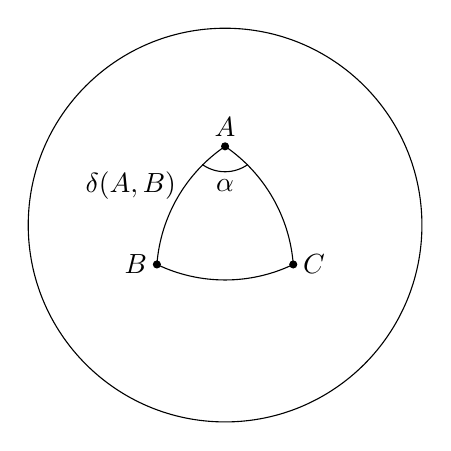
\begin{tikzpicture}
    \draw circle [radius = 2.5];
    \pgfpathmoveto{\pgfpoint{-0.86602cm}{-0.5cm}};
    \pgfpatharcto{2cm}{2cm}{0}{0}{0}{\pgfpoint{0cm}{1cm}}\pgfusepath{stroke};
    \pgfpathmoveto{\pgfpoint{0cm}{1cm}};
    \pgfpatharcto{2cm}{2cm}{0}{0}{0}{\pgfpoint{0.86602cm}{-0.5cm}}\pgfusepath{stroke};
    \pgfpathmoveto{\pgfpoint{0.86602cm}{-0.5cm}};
    \pgfpatharcto{2cm}{2cm}{0}{0}{0}{\pgfpoint{-0.86602cm}{-0.5cm}}\pgfusepath{stroke};

    \draw (0, 1) node [above] {$A$} node [draw, shape = circle, fill = black, solid, inner sep = 0, minimum size = 2.5] {};
    \draw (-0.86602, -0.5) node [left] {$B$} node [draw, shape = circle, fill = black, solid, inner sep = 0, minimum size = 2.5] {};
    \draw (0.86602, -0.5) node [right] {$C$} node [draw, shape = circle, fill = black, solid, inner sep = 0, minimum size = 2.5] {};
    \draw (-0.5, 0.5) node [left] {$\delta(A, B)$};

    \pgfpathmoveto{\pgfpoint{-0.29cm}{0.77cm}};
    \pgfpatharcto{0.5cm}{0.5cm}{0}{0}{1}{\pgfpoint{0.29cm}{0.77cm}}\pgfusepath{stroke};
    \draw (0, 0.5) node {$\alpha$};
  \end{tikzpicture}
\end{center}

Consider the circle with center $O$ containing $A$ and $B$. Arc length $AB = \angle AOB = \delta(A, B)$. Thus $a\cdot b = \cos \delta(A, B)$. $\alpha$ is the angle between planes $AOB$ and $AOC = $ angle between the normal of the two planes = angle between $\mb{a\times b}$ and $\mb{a \times c}$. Therefore
\begin{align*}
  \cos \alpha &= \mb{\frac{(a\times b)\cdot(a\times c)}{|a\times b||a\times c|}}\\
  &= \mb{\frac{b\cdot c - (a\cdot b)(a\cdot c)}{|a\times b||a\times c|}}\\
\intertext{Since $|a\times b| = \sin\delta(A, B)$, and similarly for other expressions}
  \cos\alpha\sin\delta(A, B)\sin\delta(A, C) &= \cos\delta(B, C) - \cos\delta(A, B)\cos\delta(A, C)
\end{align*}
Now consider a spherical equilateral triangle, using the spherical cosine rule, $\cos\alpha = \frac{\cos\delta - \cos^2\delta}{\sin^2\delta} = 1 - \frac{1}{1 + \cos\delta}$. Since $\cos\delta\leq 1$, then $\cos\alpha\leq \frac{1}{2}$ and $\alpha \geq 60^\circ$. With equality iff $\delta = 0$, i.e. the triangle is simply a point.

So on a sphere, each angle of an equilateral triangle is greater than $60^\circ$, and the angle sum of a triangle is greater than $180^\circ$.

\subsection{Geometry}
\subsubsection{Lines}
Any line through $\mb{a}$ and parallel to $\mb{t}$ can be written as
\[
\mb{x} = \mb{a} + \lambda\mb{t}.
\]
By crossing both sides of the equation with $\mb{t}$, we have
\begin{thm} The equation of a straight line through $a$ and parallel to $t$ is
  \[
  \mb{(x - a)\times t = 0}\text{ or }\mb{x\times t = a\times t}.
  \]
\end{thm}
\subsubsection{Plane}
To define a plane $\Pi$, we need the normal $\mb{n}$ of a plane and a fixed point $\mb{b}$.  For any $\mb{x}\in \Pi$, the vector $\mb{x - b}$ is contained in the plane and is thus normal to $\mb{n}$, i.e. $\mb{(x - b)\cdot n = 0}$.
\begin{thm}
  The equation of a plane through $b$ with normal $n$ is given by
  \[
  \mb{x\cdot n = b\cdot n}.
  \]
\end{thm}
If $\mb{n = \hat n}$, then $d = \mb{x\cdot\hat{n} = b\cdot\hat{n}}$ is the perpendicular distance from the origin to $\Pi$.

Alternatively, if $\mb{a, b, c}$ lie in the plane, then the equation of the plane is
\[
\mb{(x - a)\cdot [(b - a)\times (c - a)] = 0}.
\]

\begin{eg}\leavevmode
  \begin{enumerate}
  \item Consider the intersection between a line $\mb{x\times t = a\times t}$ with the plane $\mb{x\cdot n = b\cdot n}$. Cross $\mb{n}$ on the right with the line equation to obtain
    \[
    \mb{(x\cdot n)t - (t\cdot n)x = (a\times t)\times n}
    \]
    Eliminate $\mb{x\cdot n}$ using $\mb{x\cdot n = b\cdot n}$
    \[
    \mb{(t\cdot n)x = (b\cdot n)t - (a\times t)\times n}
    \]
    Provided $\mb{t\cdot n}$ is non-zero, the point of intersection is
    \[
    \mb{x = \frac{(b\cdot n)t - (a\times t)\times n}{t\times n}}.
    \]
    Exercise: what if $\mb{t\cdot n = 0}$?
  \item Shortest distance between two lines. Let $L_1$ be $(\mb{x} - \mb{a}_1)\times \mb{t}_1 = 0$ and $L_2$ be $(\mb{x} - \mb{a}_2)\times \mb{t}_2 = 0$.

    The distance of closest approach $s$ is along a line perpendicular to both $L_1$ and $L_2$, i.e. the line of closest approach is perpendicular to both lines and thus parallel to $\mb{t}_1\times \mb{t}_2$. The distance $s$ can then be found by projecting $\mb{a}_1 - \mb{a}_2$ onto $\mb{t}_1\times \mb{t}_2$. Thus $s = \left|(\mb{a}_1 - \mb{a}_2)\cdot\frac{\mb{t}_1\times \mb{t}_2}{|\mb{t}_1\times \mb{t}_2|}\right|$.
  \end{enumerate}
\end{eg}
\subsection{Vector equations}
\begin{eg}
  $\mb{x - (x\times a)\times b = c}$. Strategy: take the dot or cross of the equation with suitable vectors. The equation can be expanded to form
  \begin{align*}
    \mb{x - (x\cdot b)a + (a\cdot b)x} &= \mb{c}\\
    \mb{x\cdot b - (x\cdot b)(a\cdot b) + (a\cdot b)(x\cdot b)} &= \mb{c\cdot b}\\
    \mb{x\cdot b} &= \mb{c\cdot b}
  \end{align*}
  Substituting this into the original equation, we have
  \[
  \mb{x}(1 + \mb{a\cdot b}) = \mb{c + (c\cdot b)a}
  \]
  If $(1 + \mb{a \cdot b})$ is non-zero, then
  \[
  \mb{x} = \frac{\mb{c + (c\cdot b)a}}{1 + \mb{a\cdot b}}
  \]
  Otherwise, when $(1 + \mb{a\cdot b}) = 0$, if $\mb{c + (c\cdot b)a \not= 0}$, then a contradiction is reached. Otherwise, $\mb{x\cdot b = c\cdot b}$ is the most general solution, which is a plane of solutions.
\end{eg}

\section{Linear maps}
\subsection{Examples}
\subsubsection{Rotation in \texorpdfstring{$\R^3$}{R3}}
Consider a map $R: \R^3 \rightarrow \R^3$. with $\mb{x}' = R(\mb{x})$. First consider the case where this is a rotation by $\theta$ about the $z$ axis.

\begin{center}
  \begin{tikzpicture}
    \draw [->] (0, 0) -- (0, 3.5) node [pos = 1, above] {$\hat{\mb{n}}$} node [pos = 0, below] {$O$};
    \draw [->] (0, 0) -- (3, 2) node [right] {$A$} node [pos = 0.5, anchor = north west] {$\mb{x}$};
    \draw (0, 2) -- (3, 2) node [pos = 0, left] {$B$};
    \draw (0, 2) -- (2.5, 2.75) node [anchor = south west] {$A'$};
    \draw [dashed] (2.5, 2.75) -- (2.5, 2) node [below] {$C$};
    \draw [dashed, ->] (0, 0) -- (2.5, 2.75) node [pos = 0.5, anchor = south east] {$\mb{x}'$};
    \draw (2.35, 2) -- (2.35, 2.15) -- (2.5, 2.15);

    \draw (5, 2) node [left] {$B$}
    -- (7, 2) node [right] {$A$}
    -- (6.5, 3) node [above] {$A'$}
    -- cycle ;
    \draw (6.5, 3) -- (6.5, 2) node [below] {$C$};
    \draw (5.5, 2) arc(0:34:.5);
    \draw (5.5, 2) node [anchor = south west] {$\theta$};
    \draw (6.35, 2) -- (6.35, 2.15) -- (6.5, 2.15);
  \end{tikzpicture}
\end{center}

Suppose $x = (r\cos\phi, r\sin\phi, z)$. Then $x' = (r\cos(\phi + \theta), r\sin(\phi + \theta), z) = (x\cos\theta - y\sin\theta, x\sin\theta + y\cos\theta, z)$. If we say $x_i = R_{ij} x_j$, then we can have
\[
R = \begin{pmatrix}
  \cos\theta & -\sin\theta & 0 \\
  \sin\theta & \cos\theta & 0 \\
  0 & 0 & 1
\end{pmatrix}
\]
Now consider the rotation by $\theta$ by $\theta$ about $\mb{\hat{n}}$, then we have $\mb{x'} = \overrightarrow{OB} + \overrightarrow{BC} + \overrightarrow{CA'}$.
We know that
\begin{align*}
  \overrightarrow{OB} &= \mb{(\hat{n}\cdot x)\hat{n}}\\
  \overrightarrow{BC} &= \overrightarrow{BA}\cos\theta\\
  &= (\overrightarrow{BO} + \overrightarrow{OA})\cos\theta \\
  &= \mb{(-(\hat{n}\cdot x)\hat{n} + x)}\cos\theta
\end{align*}
Since we have $\overrightarrow{CA} \parallel \mb{\hat{n}\times x}$, then $|\overrightarrow{CA'}| = |\overrightarrow{BA'}|\sin\theta  = |\mb{\hat{n}\times x}|\sin\theta$ and $\overrightarrow{CA'} = \mb{(\hat{n}\times x)}\sin\theta$.

Thus $\mb{x' = x}\cos\theta + (1 - \cos\theta)\mb{(\hat{n}\cdot x)\hat{n} + \hat{n}\times x}\sin\theta$. We have
\[
x_i' = x_i\cos\theta + (1 - \cos\theta)n_jx_jn_i - \epsilon_{ijk}x_jn_k\sin\theta.
\]
We want $x_i = R_{ij}x_j$. So
\[
R_{ij} = \delta_{ij}\cos\theta + (1 - \cos\theta)n_in_j - \epsilon_{ijk}n_k\sin\theta.
\]

\subsubsection{Reflection in \texorpdfstring{$\R^3$}{R3}}
Reflect $\mb{x}$ in a plane with normal $\mb{\hat{n}}$ through $O$. The projection of $\mb{x}$ onto $\mb{\hat{n}}$ is $\mb{(x\cdot \hat{n})\hat{n}}$ . We have $\mb{x}' = \mb{x} - 2\mb{(x\cdot \hat{n})\hat{n}}$ and $x_i' = x_i - 2x_jn_jn_i$ and $R_{ij} = \delta_{ij} - 2n_in_j$.(Note: the projection  of $\mb{x}$ onto the plane is $\mb{x' = x - (x\cdot \hat{n})\hat{n}}$)

\begin{center}
  \begin{tikzpicture}
    \draw (0, 0) -- (5, 0) -- (7, 2.5) -- (2, 2.5) -- cycle;
    \draw [->] (3, 1.25) -- (3, 3) node [above] {$\hat{\mb{n}}$};
    \draw [->] (4, 1.25) -- (5, 3) node [above] {$\mb{x}$};
    \draw [dashed] (5, 3) -- (5, 1.25);
    \draw [->] (4, 1.25) -- (5, -0.5) node [below] {$\mb{x}'$};
  \end{tikzpicture}
\end{center}

\subsection{Linear Maps}
\begin{defi}[Domain, codomain and image of map]
  Consider sets $A$ and $B$ and mapping $T:A\to B$ such that $x\in A$ is mapped into a unique $x' = T(x)\in B$. $A$ is the \emph{domain} of $T$ and $B$ is the \emph{co-domain} of $T$. Typically, we have $T:\R^n \to \R^m$ or $T:\C^n\to \C^m$.
\end{defi}

\begin{defi}[Linear map]
  Let $V, W$ be real (or complex) vector spaces, and $T: V\to W$. Then $T$ is a \emph{linear map} if
  \begin{enumerate}
    \item $T(\mb{a + b}) = T(\mb{a}) + T(\mb{b})$ for all $\mb{a, b}\in V$.
    \item $T(\lambda\mb{a}) = \lambda T(\mb{A})$ for all $\lambda \in \R$ (or $\C$).
  \end{enumerate}
  Equivalently, we have $T(\lambda\mb{a} + \mu\mb{b}) = \lambda T(\mb{a}) + \mu T(\mb{b})$.
\end{defi}

\begin{eg}\leavevmode
  \begin{enumerate}
  \item Consider a translation $T:\R^3 \to \R^3$ with $T(\mb{x}) = \mb{x + a}$ for some fixed, given $\mb{a}$. This is not a linear map since $T(\lambda\mb{x} + \mu\mb{y}) = \lambda \mb{x} + \mu \mb{y} + (\lambda + \mu)\mb{a}$. Since it is not linear, there is no matrix that represents this transformation. (c.f. later lectures)
  \item Rotation, reflection and projection are linear transformations.
  \end{enumerate}
\end{eg}

\begin{defi}[Image and kernel of map]
  The \emph{image} of a map $f: U\to V$ is the subset of $V$ $\{f(\mb{u}): \mb{u}\in U\}$. The \emph{kernel} is the subset of $U$ $\{\mb{u}\in U: f(\mb{u}) = \mb{0}\}$.
\end{defi}

\begin{eg}\leavevmode
  \begin{enumerate}
  \item Consider $S: \R^3 \to \R^2$ with $S(x, y, z) = (x + y, 2x - z)$. Simple yet tedious algebra shows that this is linear.
   Now consider the effect of $S$ on the standard basis. $S(1, 0, 0) = (1, 2)$, $S(0, 1, 0) = (1, 0)$ and $S(0, 0, 1) = (0, -1)$. Clearly these are linearly dependent, but they do span the whole of $\R^2$. We can say $S(\R^3) = \R^2$. So the image is $\R^2$.

   Now solve $S(x, y, z) = 0$. We have $x + y = 0$ and $2x - z = 0$. Thus $x = (x, -x, 2x)$, i.e. vectors parallel to $(1, -1, 2)$. The set $\lambda(1, -1, 2)$ is the kernel of $S$.
   \item Consider a rotation in $\R^3$. The kernel is all vectors parallel to the axis and the image is $\R^3$.
   \item Consider a projection of $\mb{x}$ onto a plane with normal $\mb{\hat n}$. The image is the plane itself, and the kernel is any vector parallel to $\mb{\hat n}$
  \end{enumerate}
\end{eg}

\begin{thm}
  Consider a linear map $f: U\to V$, where $U, V$ are vector spaces. Then $\im (f)$ is a subspace of $V$, and $\ker (f)$ is a subspace of $U$.
\end{thm}

\begin{proof}
  Both are non-empty since $f(\mb{0}) = \mb{0}$.

  If $\mb{x, y}\in \im (f)$, then $\exists \mb{a, b}\in U$ such that $\mb{x} = f(\mb{a}), \mb{y} = f(\mb{b})$.  Then $\lambda \mb{x} + \mu\mb {y} = \lambda f(\mb{a}) + \mu f(\mb{b}) = f(\lambda\mb{a} + \mu\mb{b})$. Now $\lambda\mb{a} + \mu\mb{b}\in U$ since $U$ is a vector space, so there is an element in $U$ that maps to $\lambda\mb{x}+ \lambda\mb{y}$. So $\lambda\mb{x}+ \lambda\mb{y}\in \im (f)$ and $\im (f)$ is a subspace of $V$.

  If $\mb{x, y}\in \ker(f)$, i.e. $f(\mb{x}) = f(\mb {y}) = 0$. Then $f(\lambda\mb{x} + \mu\mb{y}) = \lambda f(\mb{x}) + \mu f(\mb{y}) = \lambda \mb{0} + \mu\mb{0} = \mb{0}$. Therefore $\lambda\mb{x}+ \mu\mb{y} \in \ker (f)$.
\end{proof}

\subsection{Rank and nullity}
\begin{defi}[Rank of linear map]
  The \emph{rank} of a linear map $f: U\to V$, denoted as $r(f)$, is the dimension of the image of $f$.
\end{defi}

\begin{defi}[Nullity of linear map]
  The \emph{nullity} of $f$, denoted $n(f)$ is the dimension of the kernel of $f$.
\end{defi}

\begin{eg}
  For the projection onto a plane in $\R^3$, the image is the whole plane and the rank is $2$. The kernel is a line so the nullity is $1$.
\end{eg}

\begin{thm}[Rank-nullity theorem]
  For a linear map $f: U \to V$,
  \[
  r(f) + n(f) = \dim (U).
  \]
\end{thm}

\begin{proof}
  (Non-examinable) Write $\dim(U) = n$ and $n(f) = m$ with $m < n$. (Note that if $m = n$, then $f$ is the zero map, and proof is trivial with $r(f) = 0$.) Suppose $(\mb{e_1, e_2\cdots e_m})$ is a basis of $\ker f$, Extend this to a basis of the whole of $U$, i.e. $(\mb{e_1, e_2, \cdots e_m, e_{m+1}, \cdots e_n})$. To prove the theorem, we need to prove that $(f(\mb{e_{m+1}}), f(\mb{e_{m + 2}}), \cdots f({\mb{e_n}}))$ is a basis of $\im (f)$.
    \begin{enumerate}
      \item First show that it spans $\im (f)$. Take $\mb{y}\in \im(f)$. Thus $\exists \mb{x}\in U$ such that $\mb{y} = f(\mb{x})$. Then
        \[
        \mb{y} = f(\alpha_1\mb{e}_1 + \alpha_2\mb{e}_2 + \cdots + \alpha_n \mb{e}_n),
        \]
        since $\mb{e}_1, \cdots \mb{e}_n$ is a basis of $U$. Thus
        \[
        y = \alpha_1f(\mb{e}_1) + \alpha_2f(\mb{e}_2) + \cdots + \alpha_m f(\mb{e}_m) + \alpha_{m + 1}f(\mb{e}_{m + 1}) + \cdots + \alpha_nf(\mb{e}_n).
        \]
        The first $m$ terms map to $\mb{0}$, since $\mb{e_1, \cdots e_m}$ is the basis of the kernel of $f$. Thus
        \[
        y = \alpha_{m + 1} f(\mb{e}_{m + 1}) + \cdots + \alpha_n f(\mb{e}_n).
        \]
      \item To show that they are linearly independent, suppose
        \[
        \alpha_{m + 1} f(\mb{e}_{m + 1}) + \cdots + \alpha_n f(\mb{e}_n) = \mb{0}.
        \]
        Then 
        \[
        f(\alpha_{m + 1}\mb{e}_{m + 1} + \cdots + \alpha_n\mb{e}_n) = \mb{0}.
        \]
        Thus $\alpha_{m + 1}\mb{e}_{m + 1} + \cdots + \alpha_n\mb{e}_n\in \ker (f)$ and for some $\alpha_1, \alpha_2, \cdots \alpha_m$, 
        \[
        \alpha_{m + 1}\mb{e}_{m + 1} + \cdots + \alpha_n\mb{e}_n = \alpha_1\mb{e_1} + \cdots + \alpha_m\mb{e}_m.
        \]
        But $\mb{e}_1\cdots \mb{e}_n$ is a basis of $U$ and are linearly independent. So $\alpha_i = 0$ for all $i$. Then the only solution to the equation $\alpha_{m + 1} f(\mb{e}_{m + 1}) + \cdots + \alpha_n f(\mb{e}_n) = \mb{0}$ is $\alpha_i = 0$, and they are linearly independent by definition.
    \end{enumerate}
\end{proof}

\begin{eg}
  Calculate the kernel and image of $f:\R^3\to \R^3$, defined by $f(x, y, z) = (x + y + z, 2x - y+ 5z, x + 2z)$.

  First find the kernel: we've got the systems of equations:
  \begin{align*}
    x + y + z &= 0\\
    2x - y + 5z &= 0\\
    x + 2z  &= 0
  \end{align*}
  Note that the first and second equation add to give $3x + 6z = 0$, which is identical to the third. Then using the first and third equation, we have $y = -x - z = z$. So the kernel is any vector in the form $(-2z, z, z)$ and is the span of $(-2, 1, 1)$.

  To find the image, extend the basis of $\ker(f)$ to a basis of the whole of $\R^3$: $(-2, 1, 1), (0, 1, 0), (0, 0, 1)$. Apply $f$ to this basis to obtain $(0, 0, 0), (1, -1, 0)$ and $(1, 5, 2)$. From the proof of the rank-nullity theorem, we know that $f(0, 0, 1)$ and $f(0, 0, 1)$ is a basis of the image.

  To get the standard form of the image, we know that the normal to the plane is parallel to $(1, -1, 0)\times (1, 5, 2) \parallel (1, 1, -3)$. Since $\mb{0}\in \im (f)$, the equation of the plane is $x + y - 3z = 0$.
\end{eg}

\subsection{Matrices}
\begin{defi}[Matrix]
  Consider a general linear map $\alpha: \R^n\to \R^m$, writing $\mb{x}' = \alpha(\mb{x})$ with $\mb{x}\in \R^n$ and $\mb{x}'\in \R^m$. Write $\mb{x} = x_j\mb{e}_j$, where $\mb{e}_i$ a is basis of $\R^n$. Then $\mb{x}' = \alpha (x_j\mb{e}_j) = x_j\alpha(\mb{e}_j)$. So $x_i' = [\alpha(\mb{e}_j)]_ix_j$. Write $x_i' = A_{ij}x_j$, with $A_{ij} = [\alpha(\mb{e}_j)]_i$. $A$ is the \emph{matrix} for $\alpha$. We write
\[
A = \{A_{ij}\} =
\begin{pmatrix}
  A_{11} & \cdots & A_{1n}\\
  \vdots & A_{ij} & \vdots\\
  A_{m1} & \cdots & A_{mn}
\end{pmatrix}
\]
We have $A_{ij}$ is in the $i$th row and $j$th column. $A$ is an $m\times n$ matrix. We can write $\mb{x'} = A\mb{x}$.
\end{defi}

\subsubsection{Examples}
\begin{enumerate}
\item Rotation by $\theta$ about $\mb{\hat k}$ (see above)
\item Reflection in plane: $R_{ij} = \delta_{ij} - 2\hat n_i\hat n_j$. Written as a matrix, we have
  \[
  \begin{pmatrix}
    1 - 2\hat{n_i}^2 & -2\hat n_1\hat n_2 & -2\hat n_1\hat n_3\\
    -2\hat n_2\hat n_1 & 1 - 2\hat n_2^2 & -2\hat n_2\hat n_3\\
    -2\hat n_3\hat n_1 & -2\hat n_3\hat n_2 & 1 - 2\hat n_3^2
  \end{pmatrix}
  \]
\item Dilation (``stretching'') $\alpha: \R^3 \to \R^3$ with $(x, y, z)\mapsto (\lambda x, \mu y, \nu z)$. The matrix is
  \[
  \begin{pmatrix}
    \lambda & 0 & 0\\
    0 & \mu & 0\\
    0 & 0 & \nu
  \end{pmatrix}
  \]
\item Shear: Consider $S:\R^3 \to \R^3$.

\begin{center}
  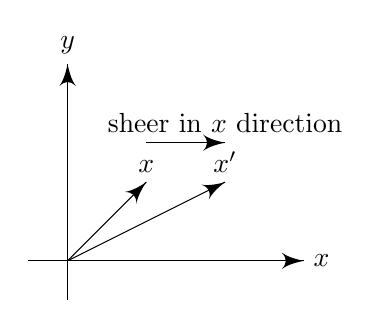
\begin{tikzpicture}
    \draw [->] (-0.5, 0) -- (3, 0) node [right] {$x$};
    \draw [->] (0, -0.5) -- (0, 2.5) node [above] {$y$};
    \draw [->] (0, 0) -- (1, 1) node [above] {$\mb{x}$};
    \draw [->] (0, 0) -- (2, 1) node [above] {$\mb{x}'$};
    \draw [->] (1, 1.5) -- (2, 1.5) node [align=center, above] {sheer in $x$ direction};
  \end{tikzpicture}
\end{center}

We have $(x, y, z)\mapsto (x + \lambda y, y, z)$. Then
\[
S =
\begin{pmatrix}
  1 & \lambda & 0\\
  0 & 1 & 0\\
  0 & 0 & 1
\end{pmatrix}
\]
\end{enumerate}

\subsubsection{Matrix Algebra}
\begin{defi}[Addition of matrices] Consider two linear maps $\alpha, \beta: \R^n\to \R^m$. The sum of $\alpha$ and $\beta$ is defined by
  \begin{align*}
    (\alpha + \beta)(\mb{x}) &= \alpha(\mb{x}) + \beta(\mb{x})\\
    \intertext{In terms of the matrix, we have}
    (A + B)_{ij}x_j &= A_{ij}x_j + B_{ij}x_j\\
    (A + B)_{ij} &= A_{ij}+B_{ij}
  \end{align*}
\end{defi}

\begin{defi}[Scalar multiplication of matrices]
  Define $(\lambda\alpha)\mb{x} = \lambda[\alpha(\mb{x})]$. So $(\lambda A)_{ij} = \lambda A_{ij}$.
\end{defi}

\begin{defi}[Matrix multiplication]
  Consider maps $\alpha: \R^\ell \to \R^n$  and $\beta: \R^n\to \R^m$. The composition is $\beta\alpha:\R^\ell\to\R^m$. Take $\mb{x}\in \R^\ell\mapsto \mb{x}''\in \R^m$. Then $\mb{x}'' = (BA)\mb{x} = B\mb{x'}$, where $\mb{x}' = A\mb{x}$. Using suffix notation, we have $x_i'' = (B\mb{x}')_i = b_{ik}x_k' = B_{ik}A_{kj}x_j$. But $x_i'' = (BA)_{ij}x_j$. So 
  \[
  (BA)_{ij} = B_{ik}A_{kj}.
  \]
  Generally, an $m\times n$ matrix multiplied by an $n\times \ell$ matrix gives an $m\times\ell$ matrix. $(BA)_{ij}$ is the $i$th row of $B$ dotted with the $j$th column of $A$.
\end{defi}
\note The number of columns of $B$ is equal to the number of rows of $A$.

\note If $\ell = m$, then both $BA$ and $AB$ makes sense, but $AB\not= BA$ in general.

\note $A(BC) = (AB)C$

\begin{defi}[Transpose of matrix]
  If $A$ is an $m\times n$ matrix, the \emph{transpose} $A^T$ is an $n\times m$ matrix defined by $(A^T)_{ij} = A_{ji}$.
\end{defi}

\begin{prop}\leavevmode
  \begin{enumerate}
  \item $(A^T)^T = A$.
  \item If $\mb{x}$ is a column vector$\begin{pmatrix}x_1\\x_2\\\vdots\\x_n\end{pmatrix}$, $\mb{x}^T$ is a row vector $(x_1\; x_2\cdots x_n)$.
  \item $(AB)^T = B^TA^T$ since $(AB)^T_{ij} = (AB)_{ji} = A_{jk}B_{kj} = B_{ki}A_{jk} $\\$= (B^T)_{ik}(A^T)_{kj} = (B^TA^T)_{ij}$.
  \end{enumerate}
\end{prop}

\begin{defi}[Hermitian conjugate]
  Define $A^{\dagger} = (A^T)^*$. Similarly, $(AB)^\dagger = B^\dagger A^\dagger$.
\end{defi}

\begin{defi}[Symmetric matrix]
  A matrix is \emph{symmetric} if $A^T = A$.
\end{defi}

\begin{defi}[Hermitian matrix]
 A matrix is \emph{Hermitian} if $A^\dagger = A$. (The diagonal of a Hermitian matrix must be real).
\end{defi}

\begin{defi}[Anti/skew symmetric matrix]
  A matrix is \emph{anti-symmetric} or \emph{skew symmetric} if $A^T = -A$. The diagonals are all zero.
\end{defi}

\begin{defi}[Skew-Hermitian matrix]
  A matrix is \emph{skew-Hermitian} if $A^\dagger = -A$. The diagonals are pure imaginary.
\end{defi}

\begin{defi}[Trace of matrix]
  The \emph{trace} of an $n\times n$ matrix $A$ is the sum of the diagonal. $\tr(A) = A_{ii}$
\end{defi}

\begin{eg}
  The reflection matrix $R_{ij} = \delta_{ij} - 2\hat n_i \hat n_j$. We have $\tr(A) = R_{ii} = 3 - 2\hat{n}\cdot \hat{n} = 3 - 2 = 1$.
\end{eg}

\begin{prop}
  $\tr(BC) = \tr(CB)$
\end{prop}

\begin{proof}
  $\tr(BC) = B_{ik}C_{ki} = C_{ki}B_{ik} = (CB)_{kk} = \tr(CB)$
\end{proof}

\begin{defi}[Identity matrix]
  $I = \delta_{ij}$.
\end{defi}

\begin{prop}
  The columns of a matrix are the images of the standard basis vectors under the mapping $\alpha$.
\end{prop}

\begin{proof}
  We have $A\mb{e}_1 = (A_{11}\; A_{21}\; \cdots A_{n1})^T$. In general, for any $i$, $A\mb{e}_i = (A_{1i}\; A_{2i}\cdots A_{ni})^T$, and the result follows.
\end{proof}

\begin{eg}
  Consider, in $\R^2$, a reflection in a line with an angle $\theta$ to the $x$ axis. We know that $\mb{\hat{i}}\mapsto \cos 2\theta \mb{\hat{i}} + \sin 2\theta\mb{\hat j}$ , with $\mb{\hat{j}}\mapsto -\cos 2\theta \mb{\hat{j}} + \sin 2\theta\mb{\hat i}$. Then the matrix is
$\begin{pmatrix}
    \cos 2\theta & \sin 2\theta\\
    \sin 2\theta & -\cos 2\theta
  \end{pmatrix}$
\end{eg}

\subsubsection{Decomposition of an \texorpdfstring{$n\times n$}{n x n} matrix}
  Any $n\times n$ matrix $B$ can be split as a sum of symmetric and antisymmetric parts. Write
\[
B_{ij} = \underbrace{\frac{1}{2}(B_{ij} + B_{ji})}_{S_{ij}} + \underbrace{\frac{1}{2}(B_{ij} - B_{ji})}_{A_{ij}}.
\]
We have $S_{ij} = S_{ji}$, so $S$ is symmetric, while $A_{ji} = -A_{ij}$, and $A$ is antisymmetric. So $B = S + A$.

Furthermore , we can decompose $S$ into an isotropic part (a scalar multiple of the identity) plus a trace-less part (i.e. sum of diagonal $= 0$). Write
\[
S_{ij} = \underbrace{\frac{1}{n}\tr (S)\delta_{ij}}_{\text{isotropic part}} + \underbrace{(S_{ij} - \frac{1}{n}\tr(S)\delta_{ij})}_{T_{ij}}.
\]
We have $\tr(T) = T_{ii} = S_{ii} - \frac{1}{n}\tr(S)\delta_{ii} = \tr(S) - \frac{1}{n}\tr(S)(n) = 0$.

Putting all these together,
\[
B = \frac{1}{n}\tr(B)I + \left\{\frac{1}{2}(B + B^T) - \frac{1}{n}\tr(B)I\right\} + \frac{1}{2}(B - B^T).
\]
In three dimensions, we can write the antisymmetric part $A$ in terms of a single vector: we have
\[
A = \begin{pmatrix}
  0 & a & -b\\
  -a & 0 & c\\
  b & -c & 0
\end{pmatrix}
\]
and we can consider
\[
\epsilon_{ijk}\omega_k =
\begin{pmatrix}
  0 & \omega_3 & -\omega_2\\
  -\omega_3 & 0 & \omega_1\\
  \omega_2 & -\omega_1 & 0
\end{pmatrix}
\]
So if we have $\mb{\omega} = (c, b, a)$, then $A_{ij} = \epsilon_{ijk}\omega_k$.

\subsubsection{Matrix inverse}

\begin{defi}[Inverse of matrix]
  Consider an $m\times n$ matrix $A$ and $n\times m$ matrices $B$ and $C$. If $BA = I$, then $B$ is the \emph{left inverse} of $A$. If $AC = I$, then $C$ is the \emph{right inverse} of $A$. If $A$ is square ($n\times n$), then $B = B(AC) = (BA)C = C$, i.e. the left and right inverses coincide. Both are denoted by $A^{-1}$, the \emph{inverse} of $A$. Therefore we have
\[
AA^{-1} = A^{-1}A = I.
\]
\end{defi}
\note Not all matrices have inverses, e.g. the zero matrix.
\begin{defi}[Invertible matrix]
  If $A$ has an inverse, then $A$ is \emph{invertible}.
\end{defi}

\begin{prop}
  $(AB)^{-1} = B^{-1}A^{-1}$
\end{prop}

\begin{proof}
  $(B^{-1}A^{-1})(AB) = B^{-1}(A^{-1}A)B = B^{-1}B = I$.
\end{proof}

\begin{defi}[Orthogonal and unitary matrices]
  A real $n\times n$ matrix is \emph{orthogonal} if $A^TA = AA^T = I$, i.e. $A^T = A^{-1}$. A complex $n\times n$ matrix is \emph{unitary} if $U^\dagger U = UU^\dagger = I$, i.e. $U^\dagger = U^{-1}$.
\end{defi}
\note An orthogonal matrix $A$ satisfies $A_{ik}(A^T_{kj}) = \delta_{ij}$, i.e. $A_{ik}A_{jk} = \delta_{ij}$. We can see this as ``the scalar product of two distinct rows is 0, and the scalar product of a row with itself is 1''. We see that the rows (and columns - by considering $A^T$) of an orthogonal matrix form an orthonormal set.

Similarly, for a unitary matrix, $U_{ik}U_{kj}^\dagger = \delta_{ij}$, i.e. $u_{ik}\overline{u_{jk}} = \overline{u_{ik}}u_{jk} =\delta_{ij}$. i.e. the rows are orthonormal, using the definition of complex scalar product.

\begin{eg}\leavevmode
  \begin{enumerate}
  \item The reflection in a plane is an orthogonal matrix. We have $R_{ij} = \delta_{ij} - 2n_in_j$. We have
    \begin{align*}
      R_{ik}R_{jk} &= (\delta_{ik} - 2n_in_k)(\delta_{jk} - 2n_jn_k)\\
      &= \delta_{ik}\delta_{jk} - 2\delta_{jk}n_in_k - 2\delta_{ik}n_jn_k + 2n_in_kn_jn_k\\
      &= \delta_{ij} - 2n_in_j - 2n_jn_i + 4n_in_j(n_kn_k)\\
      &= \delta_{ij}
    \end{align*}
  \item The rotation is an orthogonal matrix. We could multiply out using suffix notation, but it would be cumbersome to do so. Alternatively, denote rotation matrix by $\theta$ about $\mb{\hat n}$ as $R(\theta, \mb{\hat n})$. Clearly, $R(\theta, \mb{\hat n})^{-1} = R(-\theta, \mb{\hat n})$. We have
    \begin{align*}
      R_{ij}(-\theta, \mb{\hat n}) &= (\cos\theta)\delta_{ij} + n_in_j(1 - \cos\theta) + \epsilon_{ijk}n_k\sin\theta\\
      &= (\cos\theta)\delta_{ji} + n_jn_i(1 - \cos\theta) - \epsilon_{jik}n_k\sin\theta\\
      &= R_{ji}(\theta, \mb{\hat n})
    \end{align*}
    In other words, $R(-\theta, \mb{\hat n}) = R(\theta, \mb{\hat n})^T$. So $R(\theta, \mb{\hat n})^{-1} = R(\theta, \mb{\hat n})^T$.
  \end{enumerate}
\end{eg}

\subsection{Determinants}

Consider a linear map $\alpha: \R^3\to \R^3$. We have the standard basis $\mb{e}_1, \mb{e}_2, \mb{e}_3\mapsto \mb{e}_1', \mb{e}_2', \mb{e}_3'$ with $\mb{e}_i' = A\mb{e}_i$. The unit cube formed by $\mb{e}_1, \mb{e}_2, \mb{e}_3$ is mapped to the parallelopiped with volume
\begin{align*}
  [\mb{e}_1', \mb{e}_2', \mb{e}_3'] &= \epsilon_{ijk}(e_1')_i (e_2')_j (e_3')_k\\
  &= \epsilon_{ijk} A_{i\ell} \underbrace{(e_1)_\ell}_{\delta_{1\ell}} A_{jm}\underbrace{(e_2)_m}_{\delta_{2m}} A_{kn}\underbrace{(e_3)_n}_{\delta_{3n}}\\
  &= \epsilon_{ijk} A_{i1}A_{j2}A_{k3}
\end{align*}
We call this the determinant and write as
\[
\det(A) = \begin{vmatrix} A_{11} & A_{12} & A_{13}\\A_{21} & A_{22} & A_{23} \\ A_{31} & A_{32} & A_{33}\end{vmatrix}
\]

\subsubsection{Permutations}

\begin{notation}
  Consider the set $S_n$ of all permutations of $1, 2, 3, \cdots , n$. $S_n$ contains $n!$ elements. Consider $\rho\in S_n$ with $i \mapsto \rho(i)$. We write
\[
\rho = \begin{pmatrix} 1 & 2 & \cdots & n\\ \rho(1) & \rho (2) &\cdots & \rho (n)\end{pmatrix}.
\]
\end{notation}

\begin{defi}[Fixed point]
  A \emph{fixed point} of $\rho$ is a $k$ such that $\rho(k) = k$. e.g. in $\begin{pmatrix} 1 & 2 & 3 & 4\\4 & 1 & 3 & 2\end{pmatrix}$, $3$ is the fixed point. By convention, we can omit the fixed point and write as $\begin{pmatrix} 1 & 2 & 4\\ 4 & 1 & 2\end{pmatrix}$.
\end{defi}

\begin{defi}[Disjoint permutation]
  Two permutations are \emph{disjoint} if numbers moved by one are fixed by the other, and vice versa.  e.g. $\begin{pmatrix} 1 & 2 & 4 & 5 & 6\\ 5 & 6 & 1 & 4 & 2\end{pmatrix} = \begin{pmatrix}2 & 6\\ 6& 2\end{pmatrix}\begin{pmatrix}1 & 4 & 5\\5 & 1 & 4\end{pmatrix}$, and the two cycles on the right hand side are disjoint. Disjoint permutations commute, but in general non-disjoint permutations do not.
\end{defi}

\begin{defi}[Transposition and $k$-cycle]
  $\begin{pmatrix} 2 & 6 \\ 6 & 2\end{pmatrix}$ is a \emph{2-cycle} or a \emph{transposition}, and we can simply write $(2\; 6)$. $\begin{pmatrix}1 & 4 & 5\\5 & 1 & 4\end{pmatrix}$ is a 3-cycle, and we can simply write $(1\; 5\; 4)$. (1 is mapped to 5; 5 is mapped to 4; 4 is mapped to 1)
\end{defi}

\begin{prop}
  Any $q$-cycle can be written as a product of 2-cycles.
\end{prop}

\begin{defi}[Sign of permutation]
  The \emph{sign} of a permutation $\epsilon(\rho)$ is $(-1)^r$, where $r$ is the number of 2-cycles when $\rho$ is written as a product of 2-cycles. If $\epsilon(\rho) = +1$, it is an even permutation. Otherwise, it is an odd permutation. Note that $\epsilon(\rho\sigma) = \epsilon(\rho)\epsilon(\sigma)$ and $\epsilon(\rho^{-1}) = \epsilon(\rho)$.
\end{defi}

\begin{defi}[Levi-Civita symbol]
  The \emph{Levi-Civita} symbol by
\[
\epsilon_{j_1j_2\cdots j_n} = \begin{cases}+1 & \text{ if } j_1j_2j_3\cdots j_n\text{ is an even permutation of }1, 2, \cdots n\\
    -1 & \text{ if it is an odd permutation}\\
    0 & \text{ if any 2 of them are equal}
  \end{cases}
\]

Clearly, $\epsilon_{\rho(1)\rho(2)\cdots \rho(n)} = \epsilon(\rho)$.
\end{defi}

\begin{defi}[Determinant]
  The determinant of an $n\times n$ matrix $A$ is defined as:
\[
\det (A) = \sum_{\sigma\in S_n} \epsilon(\sigma) A_{\sigma(1)1}A_{\sigma(2)2}\cdots A_{\sigma(n)n},
\]
or equivalently,
\[
\det(A) = \epsilon_{j_1j_2\cdots j_n}A_{j_11}A_{j_22}\cdots A_{j_nn}.
\]
\end{defi}

\begin{prop}
  \[
  \begin{vmatrix}
    a & b\\
    c & d
  \end{vmatrix} = ad - bc
  \]
\end{prop}

\subsubsection{Properties of determinants}
\begin{prop}
  $\det (A) = \det (A^T)$.
\end{prop}

\begin{proof}
  Take a single term $A_{\sigma(1)1}A_{\sigma(2)2}\cdots A_{\sigma(n)n}$ and let $\rho$ be another permutation in $S_n$. We have
  \[
  A_{\sigma(1)1}A_{\sigma(2)2}\cdots A_{\sigma(n)n} = A_{\sigma(\rho(1))\rho(1)}A_{\sigma(\rho(2))\rho(2)}\cdots A_{\sigma(\rho(n))\rho(n)}
  \]
  since the right hand side is just re-ordering the order of multiplication. Choose $\rho = \sigma^{-1}$ and note that $\epsilon(\sigma) = \epsilon(\rho)$. Then
  \[
  \det(A) = \sum_{\rho\in S_n} \epsilon(\rho) A_{1\sigma(1)}A_{2\sigma(2)}\cdots A_{n\sigma(n)} = \det (A^T).
  \]
\end{proof}

\begin{prop}
  If matrix $B$ is formed by multiplying every element in a single row of $A$ by a scalar $\lambda$, then $\det (B) = \lambda \det (A)$. Consequently, $\det (\lambda A) = \lambda^n \det(A)$.
\end{prop}

\begin{proof}
  Each term in the sum is multiplied by $\lambda$, so the whole sum is multiplied by $\lambda$.
\end{proof}

\begin{prop}
  If 2 rows (or 2 columns) of $A$ are identical, the determinant is $0$.
\end{prop}

\begin{proof}
  wlog, suppose columns 1 and 2 are the same. Then
  \[
  \det (A) = \sum_{\sigma\in S_n} \epsilon(\sigma) A_{\sigma(1)1}A_{\sigma(2)2}\cdots A_{\sigma(n)n}.
  \]
  Now write an arbitrary $\sigma$ in the form $\sigma = \rho(1\; 2)$. Then $\epsilon(\sigma) = \epsilon(\rho)\epsilon((1\; 2)) = -\epsilon(\rho)$. So
  \[
  \det (A) = \sum_{\rho\in S_n} -\epsilon(\rho) A_{\rho(2)1}A_{\rho(1)2}A_{\rho(3)3}\cdots A_{\rho(n)n}.
  \]
  But columns 1 and 2 are identical, so $A_{\rho(2)1} = A_{\rho(2)2}$ and $A_{\rho(1)2} = A_{\rho(1)1}$. So $\det (A) = -\det (A)$ and $\det(A) = 0$.
\end{proof}

\begin{prop}
  If 2 rows or 2 columns are linearly dependent, then the determinant is zero.
\end{prop}

\begin{proof}
  Suppose in $A$, $($column $r) + \lambda($column $s) = 0$. Define
  \[
  B_{ij} =
  \begin{cases}
    A_{ij} & j\not= r\\
    A_{ij} + \lambda A_{is} & j = r
  \end{cases}.
  \]
  Then $\det (B) = \det(A) + \lambda \det($matrix with column $r =$ column $s) = \det(A)$. Then we can see that the $r$th column of $B$ is all zeroes. So each term in the sum contains one zero and $\det (A) = \det (B) = 0$.
\end{proof}
\note Even if 2 columns (or rows) are not linearly dependent, we still have $\det B = \det A$. i.e. we can add a linear multiple of a column (or row) onto another column (or row) without changing the determinant.

\begin{prop}
  $\det(AB) = \det(A)\det(B)$.
\end{prop}

\begin{proof}
  First note that $\sum_\sigma \epsilon(\sigma)A_{\sigma(1)\rho(1)}A_{\sigma(2)\rho(2)} = \epsilon(\rho)\det (A)$, i.e. swapping columns (or rows) an even/odd number of times gives a factor $\pm 1$ respectively. (Can prove by writing $\sigma = \mu \rho$)
  Now
  \begin{align*}
    \det AB &= \sum_\sigma \epsilon(\sigma)(AB)_{\sigma(1)1}(AB)_{\sigma(2)2}\cdots (AB)_{\sigma(n)}\\
    &= \sum_\sigma \epsilon(\sigma) \sum_{k_1,k_2,\cdots,k_n}^{n} A_{\sigma(1)k_1}B_{k_11}\cdots A_{\sigma(n)k_n}B_{k_nn}\\
    &= \sum_{k_1,\cdots,k_n}B_{k_11}\cdots B_{k_nn}\underbrace{\sum_\sigma \epsilon(\sigma) A_{\sigma(1)k_1}A_{\sigma(2)k_2}\cdots A_{\sigma(n)k_n}}_{S}
    \intertext{Now consider the many different $S$'s. If in $S$, two of $k_1$ and $k_n$ are equal, then $S$ is a determinant of a matrix with two columns the same, i.e. $S = 0$. So we only have to consider the sum over distinct $k_i$s. Thus the $k_i$s are are a permutation of $1, \cdots n$, say $k_i =\rho (i)$. Then we can write}
    \det AB &= \sum_\rho B_{\rho(1)1}\cdots B_{\rho(2)2} \sum_\sigma \epsilon(\sigma) A_{\sigma(1)\rho(1)} \cdots A_{\sigma(n)\rho(n)}\\
    &= \sum_\rho B_{\rho(1)1}\cdots B_{\rho(2)2} (\epsilon(\rho)\det A)\\
    &= \det A\sum_\rho \epsilon(\rho) B_{\rho(1)1}\cdots B_{\rho(2)2}\\
    &= \det A\det B
  \end{align*}
\end{proof}

\begin{cor}
  If $A$ is orthogonal, $\det A = \pm 1$.
\end{cor}

\begin{proof}
  \begin{align*}
    AA^T &= I\\
    \det AA^T &= \det I\\
    \det A\det A^T &= 1\\
    (\det A)^2 &= 1\\
    \det A &= \pm 1
  \end{align*}
\end{proof}

\begin{cor}
  If $U$ is unitary, $|\det U| = 1$
\end{cor}

\begin{proof}
  We have $\det U^\dagger = (\det U^T)^* = \det(U)^*$. Since $UU^\dagger = I$, we have $\det(U)\det(U)^* = 1$.
\end{proof}

\begin{prop}
  In $\R^3$, orthogonal matrices represent either a rotation ($\det = -1$) or a reflection ($\det = 1$).
\end{prop}
\subsubsection{Minors and Cofactors}
\begin{defi}[Minor and cofactor]
  For an $n\times n$ matrix $A$, define $A^{ij}$ to be the $(n - 1)\times (n - 1)$ matrix in which row $i$ and column $j$ of $A$ have been removed.

  The \emph{minor} of the $ij$th element of $A$ is $M_{ij} = \det A^{ij}$

  The \emph{cofactor} of the $ij$th element of $A$ is $\Delta_{ij} = (-1)^{i + j}M_{ij}$.
\end{defi}

\begin{notation}
  We use $\bar \;$ to denote a symbol which has been missed out of a natural sequence.
\end{notation}
\begin{eg}
  $1, 2, 3, 5 = 1, 2, 3, \bar 4, 5$.

\end{eg}

\begin{thm}[Laplace expansion formula]
  For any particular fixed $i$,
  \[
  \det A = \sum_{j_i = 1}^{n} A_{j_ii}\Delta_{j_ii}.
  \]
\end{thm}
\begin{proof}
  \[
  \det A = \sum_{j_i = 1}^nA_{j_ii} \sum_{j_1, \cdots, \overline{j_i}, \cdots j_n}^n \epsilon_{j_1j_2\cdots j_n} A_{j_11}A_{j_22}\cdots \overline{A_{j_ii}}\cdots A_{j_nn}
  \]
  Let $\sigma \in S_n$ be the permutation which moves $j_i$ to the $i$th position, and leave everything else in its natural order, i.e.
  \[
  \sigma =
  \begin{pmatrix}
    1 &\cdots& i & i + 1 & i + 2 & \cdots &j_{i - 1}&j_i& j_{i + 1} & \cdots n\\
    1 & \cdots & j_i & i & i + 1 & \cdots & j_{i - 2} & j_{i - 1} & j_{i + 1} & \cdots n
  \end{pmatrix}
  \]
  if $j_i > i$, and similarly for other cases. In each transposition, $|i - j_i|$ transpositions are made. So $\epsilon(\sigma) = (-1)^{i - j_i}$.

  Now consider the permutation $\rho\in S_n$
  \[
  \rho =
  \begin{pmatrix}
    1 & \cdots & \cdots & \bar {j_i} & \cdots & n\\
    j_1 & \cdots & \bar{j_i} & \cdots & \cdots & j_n\\
  \end{pmatrix}
  \]
  The composition $\rho\sigma$ reorders $(1, \cdots, n)$  to $(j_1, j_2,\cdots, j_n)$. So $\epsilon(\rho\sigma) = \epsilon_{j_1\cdots j_n} = \epsilon(\rho)\epsilon(\sigma) = (-1)^{i - j_i} \epsilon_{j_1\cdots \bar j_i \cdots j_n}$. Hence the original equation becomes

\begin{align*}
  \det A &= \sum_{j_i = 1}^n A_{j_i i} \sum_{j_1\cdots \bar j_i\cdots j_n}(-1)^{i - j_i} \epsilon_{j_1\cdots \bar j_i \cdots j_n} A_{j_11}\cdots \overline{A_{j_ii}} \cdots A_{j_nn}\\
  &= \sum_{j_i = 1}^n A_{j_ii} (-1)^{i - j_i}M_{j_ii}\\
  &= \sum_{j_i = 1}^{n} A_{j_ii}\Delta_{j_ii}
\end{align*}
\end{proof}

\begin{eg}
  $\det A = \begin{vmatrix}2 & 4 & 2\\ 3 & 2 & 1\\ 2 & 0 & 1\end{vmatrix}$. We can pick the first row and have
    \begin{align*}
      \det A&= 2\begin{vmatrix}2 & 1\\0 & 1 \end{vmatrix} - 4\begin{vmatrix} 3 & 1\\ 2 & 1\end{vmatrix} + 2\begin{vmatrix}3 & 2 \\ 2 & 0\end{vmatrix}\\
      &= 2(2 - 0) - 4(3 - 2) + 2(0 - 4)\\
      &= -8
    \end{align*}
\end{eg}

In practical terms, we use a combination of properties of determinants with a sensible choice of $i$ to evaluate $\det(A)$.

\begin{eg}
  Consider $\begin{vmatrix}1 & a & a^2\\1 & b & b^2\\1 & c & c^2 \end{vmatrix}$. Row 1 - row 2 gives
  \[
  \begin{vmatrix}0 & a - b & a^2 - b^2\\1 & b & b^2\\1 & c & c^2 \end{vmatrix} = (a - b)\begin{vmatrix}0 & 1 & a + b\\1 & b & b^2\\1 & c & c^2 \end{vmatrix}.
  \]
  Do row 2 - row 3. We obtain
  \[
  (a - b)(b - c)\begin{vmatrix}0 & 1 & a + b\\0 & 1 & b + c\\1 & c & c^2 \end{vmatrix}.
  \]
  Row 1 - row 2 gives
  \[
  (a - b)(b - c)(a - c)\begin{vmatrix}0 & 0 & 1\\0 & 1 & b + c\\1 & c & c^2 \end{vmatrix} = (a - b)(b - c)(a - c).
  \]
\end{eg}

\section{Matrices and linear equations}
\subsection{Simple example, \texorpdfstring{$2\times 2$}{2 x 2}}
Consider
\begin{align*}
A_{11}x_1 + A_{12}x_2 &= d_1\tag{a}\\
A_{21}x_1 + A_{22}x_2 &= d_2\tag{b}
\intertext{We can write as}
A\mb{x} &= \mb{d}
\end{align*}
If we do (a)$\times A_{22} - $(b)$\times A_{12}$  and similarly the other way round, we obtain
\begin{align*}
  (A_{11}A_{22} - A_{12}A_{21})x_1 &= A_{22}d_1 - A_{12}d_2\\
  \underbrace{(A_{11}A_{22} - A_{12}A_{21})}_{\det A}x_2 &= A_{11}d_2 - A_{21}d_1\\
\end{align*}
Dividing by $\det A$ and writing in matrix form, we have
\[
\begin{pmatrix}
  x_1\\
  x_2
\end{pmatrix} = \frac{1}{\det A}
\begin{pmatrix}
  A_{22} & - A_{12}\\
  -A_{21} & A_{11}
\end{pmatrix}
\begin{pmatrix}
  d_1\\
  d_2
\end{pmatrix}
\]
Given the equation $A\mb{x} = \mb{d}$, if $A^{-1}$ exists, $\mb{x} = A^{-1}\mb{d}$.

Hence, we have constructed $A^{-1}$ in the $2\times 2$ case, and show the condition for its existence is $\det A \not= 0$. with
\[
A^{-1} =\frac{1}{\det A}\begin{pmatrix}A_{22} & - A_{12}\\-A_{21} & A_{11}\end{pmatrix}
\]

\subsection{Inverse of an \texorpdfstring{$n\times n$}{n x n} matrix}
\begin{lemma}
 $\sum A_{ik}\Delta_{jk} = \delta_{ij}\det A$
\end{lemma}

\begin{proof}
  If $i \not= j$, then consider an $n\times n$ matrix $B$, which is identical to $A$ except the $j$th row is replaced by the $i$th row of $A$. So $\Delta_{jk}$ of $B = \Delta_{jk}$ of $A$, since $\Delta_{jk}$ does not depend on the elements in row $j$. Since $B$ has a duplicate row, we know that
  \[
  0 = \det B = \sum_{k = 1}^n B_{jk}\Delta_{jk} = \sum_{k = 1}^n A_{ik}\Delta_{jk}
  \]
  If $i = j$, then the expression is $\det A$ by the Laplace expansion formula.
\end{proof}

\begin{thm}
  If $\det A \not =0$, then $A^{-1}$ exists and is given by
  \[
  (A^{-1})_{ij} = \frac{\Delta_{ji}}{\det A}
  \]
\end{thm}

\begin{proof}
  \[
  (A^{-1})_{ik}A_{kj} = \frac{\Delta_{ki}}{\det A} A_{kj} = \frac{\delta_{ij}\det A}{\det A} = \delta_{ij}.
  \]
  So $A^{-1}A = I$.
\end{proof}

\begin{eg}
  Consider the shear matrix $S_\lambda = \begin{pmatrix} 1 & \lambda & 0 \\ 0 & 1 & 0\\ 0 & 0 & 1\end{pmatrix}$. We have $\det{S_\lambda} = 1$. The cofactors are\\
    \begin{tabular}{ccc}
      $\Delta_{11} = 1$       & $\Delta_{12} = 0$ & $\Delta_{13} = 0$ \\
      $\Delta_{21} - \lambda$ & $\Delta_{22} = 1$ & $\Delta_{23} = 0$ \\
      $\Delta_{31} = 0$       & $\Delta_{32} = 0$ & $\Delta_{33} = 1$
    \end{tabular}

    So $S_\lambda^{-1} = \begin{pmatrix} 1 & -\lambda & 0\\ 0 & 1 & 0\\ 0 & 0 & 1\end{pmatrix}$
\end{eg}

How many arithmetic operations are involved in calculating the inverse of an $n\times n$ matrix? We just count multiplication operations since they are the most time-consuming. Suppose that calculating $\det A$ takes $f_n$ multiplications. This involves $n$ $(n - 1)\times (n - 1)$ determinants, and you need $n$ more multiplications to put them together. So $f_n = nf_{n -1} + n$. So $f_n = O(n!)$ (In fact $f_n \approx (1 + e)n!$).

To find the inverse, we need to calculate $n^2$ cofactors. Each is a $n -1$ determinant, and each takes $O((n - 1)!)$. So the time complexity is $O(n^2 (n - 1)!) = O(n\cdot n!)$.

\subsection{Homogeneous and inhomogeneous equations}
Consider $A\mb{x} = \mb{b}$ where $A$ is an $n\times n$ matrix, $\mb{x}$ and $\mb{b}$ are $n\times 1$ column vectors.
\begin{defi}[Homogeneous equation]
  If $\mb{b} = \mb{0}$, then the system is \emph{homogeneous}. Otherwise, it's \emph{inhomogeneous}.
\end{defi}

Suppose $\det A\not= 0$. Then there is a unique solution $\mb{x} = A^{-1}\mb{b}$ ($\mb{x} = \mb{0}$ for homogeneous).

\note Recall that $\det A\not= 0$ means that the columns of $A$ are linearly independent. The columns are the images of the standard basis, $\mb{e}_i' = A\mb{e_i}$. So $\det A\not = 0$ means that $\mb{e}_i'$ are linearly independent and form a basis of $\R^n$. Therefore the image is the whole of $\R^n$. So the rank $r(A) = n$ and the nullity $n(A) = 0$. So $\det A\not= 0\Rightarrow$ kernel $= \{\mb{0}\}$.

\subsubsection{Gaussian elimination}
Consider
\begin{align*}
  A_{11}x_1 + A_{12}x_2 + \cdots + A_{1n}x_n &= d_1\\
  A_{21}x_1 + A_{22}x_2 + \cdots + A_{2n}x_n &= d_2\\
  \vdots&\\
  A_{m1}x_1 + A_{m2}x_2 + \cdots + A_{mn}x_n &= d_m
\end{align*}
So we have $m$ equations and $n$ unknowns.
Assume $A_{11}\not=0$ (if not, we can re-order the equations). We can use the first equation to eliminate $x_1$ from the remaining $(m - 1)$ equations. Then use the second equation to eliminate $x_2$ from the remaining $(m - 2)$ equations. (If anything goes wrong, just re-order until things work) Repeat.

We are left with
\begin{align*}
  A_{11}x_1 + A_{12}x_2 + A_{13}x_3 + \cdots + A_{1n}x_n &= d_1\\
  A_{22}^{(2)}x_2 + A_{23}^{(2)}x_3 + \cdots + A_{2n}^{(2)}x_n &= d_2\\
  \vdots&\\
  A_{rr}^{(r)}x_r + \cdots + A_{rn}^{(r)}x_n &= d_r\\
  0 &= d_{r + 1}^{(r)}\\
  \vdots&\\
  0 &= d_{m}^{(r)}\\
\end{align*}
Here $A_{ii}^{(i)} \not=0$ (which we can achieve by re-ordering), and the superfix $(i)$ refers to the ``version number'' of the coefficient, e.g. $A_{22}^{(2)}$ is the second version of the coefficient of $x_2$ in the second row.

Let's consider the different possibilities:
\begin{enumerate}
\item $r < m$ and at least one of $d^{(r)}_{r + 1}, \cdots d_m^{(r)} \not= 0$. Then a contradiction is reached. The system is inconsistent and has no solution. We say it is \emph{overdetermined}.
  \begin{eg}
    Consider the system
    \begin{align*}
      3x_1 + 2x_2 + x_3 &= 3\\
      6x_1 + 3x_2 + 3x_3 &= 0\\
      6x_1 + 2x_2 + 4x_3 &= 6
    \intertext{This becomes }
      3x_1 + 2x_2 + x_3 &= 3\\
      0 - x_2 + x_3 &= -6\\
      0 - 2x_2 + 2x_3 &= 0
    \intertext{And then}
      3x_1 + 2x_2 + x_3 &= 3\\
      0 - x_2 + x_3 &= -6\\
      0 &= 12
    \end{align*}
    We have $d_3^{(3)} = 12 = 0$ and there is no solution.
  \end{eg}
  \item If $r = n\leq m$, and all $d_{r + i}^{(r)} = 0$. Then from the $n$th equation, there is a unique solution for $x_n = d_{n}^{(n)}/A_{nn}^{(n)}$, and hence for all $x_i$ by back substitution. This system is \emph{determined}.
    \begin{eg}
      \begin{align*}
        2x_1 + 5x_2 &= 2\\
        4x_1 + 3x_2 &= 11\\
        \intertext{This becomes}
        2x_1 + 5x_2 &= 2\\
        -7x_2 &= 7
      \end{align*}
      So $x_2 = -1$ and thus $x_1 = 7/2$.
    \end{eg}
  \item If $r < n$ and $d_{r + i}^{(r)} = 0$, then $x_{r + 1}, \cdots x_n$ can be freely chosen, and there are infinitely many solutions. System is \emph{under-determined}. e.g.
    \begin{align*}
      x_1 + x_2 &= 1\\
      2x_1 + 2x_2 &= 2
      \intertext{Which gives}
      x_1 + x_2 &= 1\\
      0 &= 0
    \end{align*}
    So $x_1 = 1 - x_2$ is a solution for any $x_2$.
\end{enumerate}
\note In the $n = m$ case, there are $O(n^3)$ operations involved, which is much less than inverting the matrix.

Relation to determinant: when $m = n$, then the number of equations is equal to the number of unknowns. Then $A$ is square. We have
\[
\det A  = (-1)^k
\begin{vmatrix}
  A_{11} &A_{12}&\cdots& \cdots& \cdots & A_{1n}\\
  0 & A_{22}^{(2)} &\cdots& \cdots & \cdots & A_{2n}^{(n)} \\
  \vdots & \vdots &\ddots & \vdots & \vdots & \vdots\\
  0 & 0 & \cdots & A_{rr}^{(r)} & \cdots & A_{rn}^{(n)}\\
  0 & 0 & \cdots & 0 & 0 & \cdots\\
  \vdots & \vdots & \vdots & \vdots & \vdots & \vdots
\end{vmatrix}
\]
where the $(-1)^k$ arises due to the swapping of rows.

This determinant is an \emph{upper triangular} one (all elements below diagonal $= 0$) and the determinant is the product of its diagonal elements.
Hence if $r < n$ (and $d_i^{(r)} = 0$ for $i > r$), then we have case (ii) and the $\det A = 0$. If $r = n$, then $\det A = (-1)^k A_{11}A_{22}^{(2)}\cdots A_{rr}^{(r)} \not= 0$.

\subsection{Matrix rank}
Consider a linear map $\alpha: \R^n\to \R^m$. Recall the rank $r(\alpha)$ is the dimension of the image. Suppose that the matrix $A$ is associated with the linear map. We also call $r(A)$ the \emph{rank} of $A$.

Recall that if the standard basis is $\mb{e}_1,\cdots \mb{e}_n$, then $A\mb{e}_1, \cdots, A\mb{e}_n$ span the image (but not necessarily linearly independent).

Further, $A\mb{e}_1, \cdots, A\mb{e}_n$ are the columns of the matrix $A$. Then $r(A)$ is the number of linearly independent columns.

\begin{defi}[Column and row rank of linear map]
  The \emph{column rank} of a matrix is the maximum number of linearly independent columns.

The \emph{row rank} of a matrix is the maximum number of linearly independent rows.
\end{defi}

\begin{thm}
  The column rank and row rank are equal for any $m\times n$ matrix.
\end{thm}

\begin{proof}
  Let $r$ be the row rank of $A$. Write the biggest set of linearly independent rows as $\mb{v}_1^T, \mb{v}_2^T, \cdots \mb{v}_r^T$ or in component form $\mb{v}_k^T = (v_{k1}, v_{k2}, \cdots, v_{kn})$ for $k = 1, 2, \cdots, r$.

Now denote the $i$th row of $A$ as $\mb{r}_i^T = (A_{i1}, A_{i2}, \cdots A_{in})$.

Note that every row of $A$ can be written as a linear combination of the $\mb{v}$'s. (If $\mb{r_i}$ cannot be written as a linear combination of the $\mb{v}$'s, then it is independent of the $\mb{v}$'s and $\mb{v}$ is not the maximum collection of linearly independent rows) Write
\[
\mb{r}_i^T = \sum_{k = 1}^r C_{ik}\mb{v}_{k}^T.
\]
For some coefficients $C_{ik}$ with $i \leq i\leq m$ and $1 \leq k \leq r$.

Now the elements of $A$ are
\[
A_{ij} = (\mb{r}_i)^T_j = \sum_{k = 1}^r C_{ik}(\mb{v}_k)_j,
\]
or
\[
\begin{pmatrix}
  A_{1j}\\
  A_{2j}\\
  \vdots\\
  A_{mj}
\end{pmatrix} = \sum_{k = 1}^r {\mb{v}_k}_j
\begin{pmatrix}
  C_{1k}\\
  C_{2k}\\\
  \vdots\\
  C_{mk}
\end{pmatrix}
\]

So every column of $A$ can be written as a linear combination of the $r$ column vectors $\mb{c}_k$. Then the column rank of $A \leq r$, the row rank of $A$.

Apply the same argument to $A^T$ to see that the row rank is $\leq$ the column rank.
\end{proof}

\subsection{Homogeneous problem \texorpdfstring{$A\mb{x} = \mb{0}$}{Ax = 0}}
We restrict our attention to the square case, i.e. number of unknowns = number of equations, $A$ is an $n\times n$ matrix. We want to solve $A\mb{x} = \mb{0}$.

First of all, if $\det A\not=0$, then $A^{-1}$ exists and $\mb{x}^{-1} = A^{-1}\mb{0} = \mb{0}$, which is the unique solution. Hence if $A\mb{x} = \mb{0}$ with $\mb{x} \not= \mb{0}$, then $\det A = 0$.

\subsubsection{Geometrical interpretation}
We consider a $3\times 3$ matrix
\[
A = \begin{pmatrix} \mb{r}_1^T\\\mb{r}_2^T\\\mb{r}_3^T\end{pmatrix}
\]
$A\mb{x} = \mb{0}$ means that $\mb{r}_i^T\cdot \mb{x} = 0$ for all $i$. Note that this represents three planes through the origin. The solution is the intersection of the three planes that go through the origin.

There are three possibilities:
\begin{enumerate}
\item If $\det A =[\mb{r}_1, \mb{r}_2, \mb{r}_3] \not= 0$, span$\{\mb{r}_1, \mb{r}_2, \mb{r}_3\} = \R^3$ and thus $r(A) = 3$. By the rank-nullity theorem, $n(A) = 0$ and the kernel is $\{\mb{0}\}$. So $\mb{x} = \mb{0}$ is the unique solution.
\item If $\det A = 0$, then  $\dim(\spn\{\mb{r}_1, \mb{r}_2, \mb{r}_3\}) = 1$ or $2$.
  \begin{enumerate}
  \item If rank $= 2$, wlog assume $\mb{r}_1, \mb{r}_2$ are linearly independent. So $\mb{x}$ lies on the intersection of two planes $\mb{x}\cdot \mb{r}_1 = 0$ and $\mb{x}\cdot \mb{r}_2 = 0$, which is the line $\{\mb{x}\in \R^3: \mb{x} = \lambda \mb{r}_1\times \mb{r}_2\}$ (Since $\mb{x}$ lies on the intersection of the two planes, it has to be normal to the normals of both planes). All such points on this line also satisfy $\mb{x}\cdot\mb{r}_3 = 0$ since $\mb{r}_3$ is a linear combination of $\mb{r}_1$ and $\mb{r}_2$. The kernel is a line, $n(A) = 1$.
  \item If rank = 1, then $\mb{r}_1, \mb{r}_2, \mb{r}_3$ are parallel. So $\mb{x}\cdot \mb{r}_1 = 0 \Rightarrow \mb{x}\cdot \mb{r}_2 = \mb{x}\cdot \mb{r}_3 = 0$. So all $\mb{x}$ that satisfy $\mb{x}\cdot \mb{r}_1 = 0$ are in the kernel, and the kernel now is a plane. $n(A) = 2$.
  \end{enumerate}
\end{enumerate}
(We also have the trivial case where $r(A) = 0$, we have the zero mapping and the kernel is $\R^3$)

\subsubsection{Linear mapping view of \texorpdfstring{$A\mb{x} = \mb{0}$}{Ax = 0}}
Consider a linear map $\alpha: \R^n \to \R^n$ $\mb{x} \mapsto \mb{x}' = A\mb{x}$. The kernel $k(A) = \{x\in \R^n: A\mb{x} = \mb{0}\}$ has dimension $n(A)$.

\begin{enumerate}
\item If $n(A) = 0$, then $A(\mb{e}_1), A(\mb{e}_2), \cdots, A(\mb{e}_n)$ is a linearly independent set, and $r(A) = n$.
\item If $n(A) > 0$, then $\{\mb{u}_i\}, i = 1, \cdots, n(A)$ is a basis of the kernel. So given any solution to $A\mb{x} = \mb{0}$, $\displaystyle \mb{x} = \sum_{i = 1}^{n(A)} \lambda_i \mb{u}_i$. Extend $\{\mb{u}_i\}$ to be a basis of $\R^n$ by introducing extra vectors $\mb{u}_{i}$ for $i = n(A) + 1, \cdots, n$. The vectors $A(\mb{u}_i)$ for $i = n(A) + 1, \cdots, n$ form a basis of the image.
\end{enumerate}

\subsection{General solution of \texorpdfstring{$A\mb{x} = \mb{d}$}{Ax = d}}
Where $A$ is an $n\times n$ matrix with $\mb{x, d}$ being $n \times 1$ column vectors.

\begin{enumerate}
\item $\det(A) \not= 0$. So $A^{-1}$ exists and $n(A) = 0$, $r(A) = n$. Then for any $\mb{d}\in \R^n$, a unique solution must exists and it is $\mb{x} = A^{-1}\mb{d}$.
\item $\det(A) = 0$. Then $A^{-1}$ does not exist, and $n(A) > 0$, $r(A) < n$. Since the image of $A$ is not the whole of $\R^n$.
  \begin{enumerate}
  \item If $\mb{d}\not\in \im A$, then there is no solution (by definition of the image)
  \item If $\mb{d}\in \im A$, then by definition there exists at least one $\mb{x}$ such that $A\mb{x} = \mb{d}$. The general solution of $A\mb{x} = \mb{d}$  can be written as $\mb{x} = \mb{x}_0 + \mb{y}$, where $\mb{x}_0$ is a particular solution (i.e. $A\mb{x}_0 = \mb{d}$), and $\mb{y}$ is any vector in $\ker A$ (i.e. $A\mb{y} = \mb{0}$). (c.f. Isomorphism theorem)

    If $n(A) = 0$, then $\mb{y = 0}$ only, and then the solution is unique (i.e. case (i)). If $n(A) > 0$ , then $\{\mb{u}_i\}, i = 1, \cdots, n(A)$ is a basis of the kernel.
\[
\mb{y} = \sum_{j = 1}^{n(A)} \mu_j \mb{u}_j,
\]
so
\[
\mb{x} = \mb{x}_0 + \sum_{j = 1}^{n(A)} \mu_j \mb{u}_j
\]
for any $\mu_j$, i.e. there are infinitely many solutions.
  \end{enumerate}
\end{enumerate}
\begin{eg}
  \[
  \begin{pmatrix}
    1 & 1\\
    a & 1
  \end{pmatrix}
  \begin{pmatrix}
    x_1\\
    x_2
  \end{pmatrix} =
  \begin{pmatrix}
    1\\
    b
  \end{pmatrix}
  \]
  We have $\det A = 1 - a$. If $a \not= 1$, then $A^{-1}$ exists and
  \[
  A^{-1} = \frac{1}{1 - a} = \frac{1}{1 - a}\begin{pmatrix}
    1 & -1\\
    -a & 1
  \end{pmatrix}.
  \]
  Then
  \[
  \mb{x} = \frac{1}{1- a}\begin{pmatrix}
    1 - b\\
    -a + b
  \end{pmatrix}.
  \]
  If $a = 1$, then
  \[
  A\mb{x} = \begin{pmatrix}
    x_1 + x_2\\
    x_1 + x_2
  \end{pmatrix} = (x_1 + x_2)\begin{pmatrix}
    1\\
    1
  \end{pmatrix}.
  \]
  So $\im A = \spn\left\{
  \begin{pmatrix}
    1\\1
  \end{pmatrix}
  \right\}$ and $\ker A = \spn\left\{
  \begin{pmatrix}
    1\\-1
  \end{pmatrix}
  \right\}$. If $b \not=1 $, then $\begin{pmatrix}
    1\\b
  \end{pmatrix}
  \not\in \im A$ and there is no solution. If $b = 1$, then $
  \begin{pmatrix}
    1\\b
  \end{pmatrix}
  \in \im A$.

  We find a particular solution of
  $\begin{pmatrix}
    1\\
    0
  \end{pmatrix}$. So The general solution is
  \[
  \mb{x} =
  \begin{pmatrix}
    1\\0
  \end{pmatrix}
  + \lambda
  \begin{pmatrix}
    1\\-1
  \end{pmatrix}.
  \]
\end{eg}

\begin{eg}
  Find the general solution of
  \[
  \begin{pmatrix}
    a & a & b\\
    b & a & a\\
    a & b & a
  \end{pmatrix}
  \begin{pmatrix}
    x\\y\\z
  \end{pmatrix}
  =\begin{pmatrix}
   1\\c\\1
  \end{pmatrix}
  \]

  We have $\det A = (a - b)^2 (2a + b)$. If $a \not= b$ and $b \not= -2a$, then the inverse exists and there is a unique solution for any $c$.
  \begin{enumerate}
  \item $a = b, b \not= -2a$. So $a\not= 0$. The kernel is the plane $x + y + z = 0$ which is $\spn\left\{
    \begin{pmatrix}
      -1\\1\\0
    \end{pmatrix},
    \begin{pmatrix}
      -1\\ 0\\ 1
    \end{pmatrix}\right\}$
    We extend this basis to $\R^3$ by adding $
    \begin{pmatrix}
      1\\0\\0
    \end{pmatrix}$.

    So the image is the span of $
    \begin{pmatrix}
      a\\a\\a
    \end{pmatrix} =
    \begin{pmatrix}
      1\\1\\1
    \end{pmatrix}$. Hence if $c\not= 1$, then $
    \begin{pmatrix}
      1\\c\\1
    \end{pmatrix}$ is not in the image and there is no solution.  If $c = 1$, then a particular solution is $
    \begin{pmatrix}
      \frac{1}{a}\\0\\0
    \end{pmatrix}$
    and the general solution is
    \[
    \mb{x} =
    \begin{pmatrix}
      \frac{1}{a}\\0\\0
    \end{pmatrix} + \lambda
    \begin{pmatrix}
      -1\\1\\0
    \end{pmatrix} + \mu
    \begin{pmatrix}
      -1\\0\\1
    \end{pmatrix}
    \]
  \item If $a\not= b$ and $b = -2a$, then $a \not= 0$. The kernel satisfies
    \begin{align*}
      x + y - 2z &= 0\\
      -2x + y + z &= 0\\
      x - 2y + z &= 0
    \end{align*}
    This can be solved to give $x = y = z$, and the kernel is $\spn\left\{
    \begin{pmatrix}
      1\\1\\1
    \end{pmatrix}\right\}$. We add $
    \begin{pmatrix}
      1\\0\\0
    \end{pmatrix}$ and $
    \begin{pmatrix}
      0\\0\\1
    \end{pmatrix}$ to form a basis of $\R^3$. So the image is the span of $
    \begin{pmatrix}
      1\\-2\\1
    \end{pmatrix},
    \begin{pmatrix}
      -2\\1\\1
    \end{pmatrix}$.

    If $
    \begin{pmatrix}
      1\\c\\1
    \end{pmatrix}$ is in the image, then
    \[
    \begin{pmatrix}
      1\\c\\1
    \end{pmatrix} = \lambda
    \begin{pmatrix}
      1\\-2\\1
    \end{pmatrix}
    + \mu
    \begin{pmatrix}
      -2\\1\\1
    \end{pmatrix}.
    \]
    Then the only solution is $\mu = 0, \lambda = 1, c = -2$. Thus there is no solution if $c \not= -2$, and when $c = -2$, pick a particular solution $
    \begin{pmatrix}
      \frac{1}{a}\\0\\0
    \end{pmatrix}$ and the general solution is
    \[
    \mb{x} = \begin{pmatrix}
      \frac{1}{a}\\0\\0
    \end{pmatrix} +\lambda
    \begin{pmatrix}
      1\\1\\1
    \end{pmatrix}
    \]
    \item If $a = b$ and $b = -2a$, then $a = b = 0$ and $\ker A = \R^3$. So there is no solution for any $c$.
\end{enumerate}
\end{eg}

\section{Eigenvalues and eigenvectors}
\subsection{Preliminaries and definitions}
\begin{thm}[Fundamental theorem of algebra]
  Consider polynomial $p(z)$ of degree $m \geq 1$, i.e.
  \[
  p(z) = \sum_{j = 0}^m c_jz^j,
  \]
  where $c_j\in \C$ and $c_m \not= 0$.

  Then $p(z) = 0$ has precisely $m$ (not necessarily distinct) roots in the complex roots, accounting for multiplicity.
\end{thm}

\begin{defi}[Multiplicity of root]
  The root $z = \omega$ has \emph{multiplicity} $k$ if $(z - \omega)^k$ is a factor of $p(z)$ but $(z - \omega)^{k + 1}$ is not.
\end{defi}

\begin{eg}
  When $p(z) = z^3 - z^2 - z + 1 = (z - 1)^2(z + 1)$. So $p(z) = 0$ has roots $1, 1, -1$, where $z = 1$ has multiplicity $2$.
\end{eg}

\begin{defi}[Eigenvector and eigenvalue]
  Consider a linear map $\alpha: \C^n\to \C^n$ with associated matrix $A$. Then $\mb{x}\not= \mb{0}$ is an eigenvector of $A$ if
  \[
  A\mb{x} = \lambda\mb{x}
  \]
  for some $\lambda$. $\lambda$ is the associated \emph{eigenvalue}. This means that the direction of the eigenvector is preserved by the mapping, but is scaled up by $\lambda$.
\end{defi}

\begin{thm}
  $\lambda$ is an eigenvalue of $\lambda$ iff
  \[
  \det(A - \lambda I) = 0.
  \]
\end{thm}

\begin{proof}
  $(\Rightarrow)$ We can rearrange the equation in the definition above to
  \[
  (A - \lambda I)\mb{x} = \mb{0}
  \]
  and thus
  \[
  \mb{x}\in \ker(A - \lambda I)
  \]
  But $\mb{x}\not= \mb{0}$. So $\ker(A - \lambda I)$ is non-trivial and $\det(A - \lambda I) = 0$. The $(\Leftarrow)$ direction is similar. 
\end{proof}

\begin{defi}[Characteristic equation of matrix]
  The \emph{characteristic equation} of $A$ is
  \[
  \det(A - \lambda I) = 0
  \]
\end{defi}

\begin{defi}[Characteristic polynomial of matrix]
  The \emph{characteristic polynomial} of $A$ is
  \[
  p_A(\lambda) = \det(A - \lambda I).
  \]
\end{defi}

From the definition of the determinant,
\begin{align*}
  p_A(\lambda) &= \det(A - \lambda I)\\
  &= \epsilon_{j_1j_2\cdots j_n} (A_{j_1 1} - \lambda\delta_{j_11})\cdots (A_{n_1 n} - \lambda\delta_{j_nn})\\
  &= c_0 + c_1\lambda + \cdots + c_n\lambda^n
\end{align*}
Note the following:
\begin{enumerate}
\item $p_A(\lambda)$ has degree $n$ and has $n$ roots. So an $n\times n$ matrix has $n$ eigenvalues (accounting for multiplicity).
\item If $A$ is real, then all $c_i\in \R$. So eigenvalues are either real or come in complex conjugate pairs.
\item $c_n = (-1)^n$ and $c_{n - 1} = (-1)^{n - 1}(A_{11} + A_{22} + \cdots + A_{nn}) = (-1)^{n - 1}\tr(A)$. But $c_{n -1}$ is the sum of roots, i.e. $c_{n - 1}= (-1)^{n - 1}(\lambda_1 + \lambda_2 + \cdots \lambda_n)$, so
\[
\tr(A) = \lambda_1 + \lambda_2 + \cdots + \lambda_n.
\]
Finally, $c_0 = p_A(0) = \det(A)$. Also $c_0$ is the product of all roots, i.e. $c_0 = \lambda_1\lambda_2\cdots \lambda_n$. So
\[
\det A = \lambda_1\lambda_2\cdots \lambda_n.
\]
\end{enumerate}

The kernel of the matrix $A - \lambda I$ is the set $\{\mb{x}: A\mb{x} = \lambda\mb{x}\}$. This is a vector subspace because the kernel of any map is always a subspace.

\begin{defi}[Eigenspace]
  The \emph{eigenspace} denoted as $E_\lambda$ is the kernel of the matrix $A - \lambda I$, i.e. the set of eigenvectors with eigenvalue $\lambda$.
\end{defi}

\begin{defi}[Algebraic multiplicity of eigenvalue]
  The \emph{algebraic multiplicity} $M(\lambda)$ or $M_\lambda$ of an eigenvalue $\lambda$ is the multiplicity of $\lambda$ in $p_A(\lambda) = 0$. Clearly (by the fundamental theorem of algebra),
  \[
  \sum_\lambda M(\lambda) = n.
  \]
  If $M(\lambda) > 1$, then the eigenvalue is \emph{degenerate}.
\end{defi}

\begin{defi}[Geometric multiplicity of eigenvalue]
  The \emph{geometric multiplicity} $m(\lambda)$ or $m_\lambda$ of an eigenvalue $\lambda$ is the dimension of the eigenspace, i.e. the maximum number of linearly independent eigenvectors with eigenvalue $\lambda$.
\end{defi}

\begin{defi}[Defect of eigenvalue]
  The \emph{defect} $\Delta_\lambda$ of eigenvalue $\lambda$ is
  \[
  \Delta_\lambda = M(\lambda) - m(\lambda).
  \]
  It can be proven that $\Delta_\lambda > 0$.
\end{defi}

\subsection{Linearly independent eigenvectors}
\begin{thm}
  Suppose $n\times n$ matrix $A$ has \emph{distinct} eigenvalues $\lambda_1, \lambda_2, \cdots, \lambda_n$. Then the corresponding eigenvectors $\mb{x}_1, \mb{x}_2, \cdots, \mb{x}_n$ are linearly independent.
\end{thm}

\begin{proof}
  Proof by contradiction: Suppose $\mb{x}_1, \mb{x}_2, \cdots, \mb{x}_n$ are linearly dependent. Then we can find non-zero constants $d_i$ for $i = 1, 2, \cdots, r, d_i\not= 0$, such that
  \[
  d_1\mb{x}_1 + d_2\mb{x}_2 + \cdots + d_r\mb{x}_r = \mb{0}.
  \]
  Suppose that this is the shortest non-trivial linear combination that gives $\mb{0}$ (we may need to re-order $\mb{x}_i$).

  Now apply $(A - \lambda_1 I)$ to the whole equation to obtain
  \[
  d_1(\lambda_1 - \lambda_1)\mb{x}_1 + d_2(\lambda_2 - \lambda_1)\mb{x}_2 + \cdots + d_r(\lambda_r - \lambda_1)\mb{x}_r = \mb{0}.
  \]
  We know that the first term is $\mb{0}$, while the others are not (since we assumed $\lambda_i \not= \lambda_j$ for $i\not= j$). So
  \[
  d_2(\lambda_2 - \lambda_1)\mb{x}_2 + \cdots + d_r(\lambda_r - \lambda_1)\mb{x}_r = \mb{0},
  \]
  and we have found a shorter linear combination that gives $\mb{0}$. Contradiction.
\end{proof}

\begin{eg}\leavevmode
  \begin{enumerate}
  \item $A = \begin{pmatrix} 0 & 1\\
    -1 & 0
  \end{pmatrix}$. Then $p_A(\lambda) = \lambda^2 + 1 = 0$. So $\lambda_1 = i$ and $\lambda_1 = -i$.

    To solve $(A - \lambda_1 I)\mb{x} = \mb{0}$, we obtain
    \[
    \begin{pmatrix}
      -i & 1\\-1 & -i
    \end{pmatrix}
    \begin{pmatrix}
      x_1\\x_2
    \end{pmatrix}
     = \mb{0}.
     \]
     So we obtain
     \[
     \begin{pmatrix}
       x_1\\x_2
     \end{pmatrix} =
     \begin{pmatrix}
       1\\i
     \end{pmatrix}
     \]
     to be an eigenvector. Clearly any scalar multiple of $\begin{pmatrix}
       1\\i
     \end{pmatrix}$ is also a solution, but still in the same eigenspace $E_i = \spn \begin{pmatrix}
       1\\i
     \end{pmatrix}$

     Solving $(A - \lambda_2I)\mb{x} = \mb{0}$ gives 
     \[
     \begin{pmatrix}
       x_1\\x_2
     \end{pmatrix} =
     \begin{pmatrix}
       1\\-i
     \end{pmatrix}.
     \]
     So $E_{-i} = \spn
     \begin{pmatrix}
       1\\-i
     \end{pmatrix}$.

     Note that $M(\pm i) = m(\pm i) = 1$, so $\Delta_{\pm i} = 0$. Also note that the two eigenvectors are linearly independent and form a basis of $\C^2$.
   \item Consider
     \[
     A = \begin{pmatrix}
     -2 & 2 & -3\\
     2 & 1 & -6\\
     -1 & -2 & 0
     \end{pmatrix}
     \]
     Then $\det(A - \lambda I) = 0$ gives $45 + 21\lambda - \lambda^2 - \lambda^3$. So $\lambda_1 = 5, \lambda_2 = \lambda_3 = -3$.

     The eigenvector with eigenvalue $5$ is
     \[
     \mb{x} =
     \begin{pmatrix}
       1\\2\\-1
     \end{pmatrix}
     \]

     We can find that the eigenvectors with eigenvalue $-3$ are
     \[
     \mb{x} =
     \begin{pmatrix}
       -2x_2 + 3x_3\\x_2\\x_3
     \end{pmatrix}
     \]
     for any $x_2, x_3$. This gives two linearly independent eigenvectors, say $
     \begin{pmatrix}
       -2\\1\\0
     \end{pmatrix},
     \begin{pmatrix}
       3\\0\\1
     \end{pmatrix}$.

     So $M(5) = m(5) = 1$ and $M(-3) = m(-3) = 2$, and there is no defect for both of them. Note that these three eigenvectors form a basis of $\C^3$.
   \item Let
     \[
     A = \begin{pmatrix}
       -3&-1&1\\
       -1 & -3 & 1\\
       -2 & -2 & 0
     \end{pmatrix}
     \]
     Then $0 = p_A(\lambda) = -(\lambda+2)^4$. So $\lambda = -2, -2, -2$. To find the eigenvectors, we have
     \[
     (A + 2I)\mb{x} = 
     \begin{pmatrix}
       -1&-1&1\\
       -1 & -1 & 1\\
       -2 & -2 & 2
     \end{pmatrix}
     \begin{pmatrix}
       x_1\\x_2\\x_3
     \end{pmatrix}
     = \mb{0}
     \]
     The general solution is thus $x_1 + x_2 - x_3 = 0$, and the general solution is thus $x = 
     \begin{pmatrix}
       x_1\\x_2\\x_1 + x_2
     \end{pmatrix}$. The eigenspace $E_{-2} = \spn\left\{
     \begin{pmatrix}
       1\\0\\1
     \end{pmatrix}, 
     \begin{pmatrix}
       0\\1\\1
     \end{pmatrix}\right\}$.

     Hence $M(-2) = 3$ and $m(-2) = 2$. Thus the defect $\Delta_{-2} = 1$. So the eigenvectors do not form a basis of $\C^3$.
   \item Consider the reflection $R$ in the plane with normal $\mb{n}$. Clearly $R\mb{n} = -\mb{n}$. the eigenvalue is $-1$ and the eigenvector is $\mb{n}$. Then $E_1 = \spn\{\mb{n}\}$. So $M(-1) = m(-1) = 1$.

     If $\mb{p}$ is any vector in the plane, $R\mb{p} = \mb{p}$. So this has an eigenvalue of $1$ and eigenvectors being any vector in the plane. So $M(1) = m(1) = 2$.

     So the eigenvectors form a basis of $\R^3$.
   \item Consider a rotation $R$ by $\theta$ about $\mb{n}$. Since $R\mb{n} = \mb{n}$, we have an eigenvalue of $1$ and eigenspace $E_1 = \spn\{\mb{n}\}$.

     We know that there are no other real eigenvalues since rotation changes the direction of any other vector. The other eigenvalues turn out to be $e^{\pm i\theta}$. If $\theta \not= 0$, there are 3 distinct eigenvalues and the eigenvectors form a basis of $\C^3$.
   \item Consider a shear
     \[
     A = 
     \begin{pmatrix}
       1&\mu\\0&1
     \end{pmatrix}
     \]
     The characteristic equation is $(1 - \lambda)^2 = 0$ and $\lambda = 1$. The eigenvectors corresponding to $\lambda = 1$ is $\mb{x} = 
     \begin{pmatrix}
       1\\0
     \end{pmatrix}$. We have $M(1) = 2$ and $m(1) = 1$. So $\Delta_1 = 1$.
  \end{enumerate}
\end{eg}
\note If $n\times n$ matrix $A$ has $n$ distinct eigenvalues, and hence has $n$ linearly independent eigenvectors $\mb{v}_1, \mb{v}_2, \cdots \mb{v}_n$, then \emph{with respect to this eigenvector basis}, $A$ is diagonal.

In this basis, $v_1 = (1, 0, \cdots, 0)$ etc. We know that $A\mb{v}_i = \lambda_i\mb{v}_i$ (no summation). So the image of the $i$th basis vector is $\lambda_i$ times the $i$th basis. Since the columns of $A$ are simply the images of the basis,
\[
\begin{pmatrix}
  \lambda_1 & 0 & \cdots & 0\\
  0 & \lambda_2 & \cdots & 0\\
  \vdots & \vdots & \ddots & \vdots\\
  0 & 0 & \cdots & \lambda_n
\end{pmatrix}
\]
\note $\tr A = \lambda_1 + \lambda_2 + \cdots + \lambda_n$ and $\det(A) = \lambda_1\lambda_2\cdots \lambda_n$ in this basis as well.

The fact that $A$ can be diagonalized in this base by changing the basis is an important observation.

\subsection{Transformation matrices}
How do the components of a vector or a matrix change when we change the basis?

Let $\{\mb{e}_1, \mb{e}_2, \cdots, \mb{e}_n\}$ and $\{\tilde{\mb{e}}_1, \tilde{\mb{e}}_2,\cdots,  \tilde{\mb{e}}_n\}$ be 2 different bases of $\R^n$ or $\C^n$. Then we can write
\[
\tilde{\mb{e}_j} = \sum_{i = 1}^n P_{ij}\mb{e}_i
\]
i.e. $P_{ij}$ is the $i$th component of $\tilde{\mb{e}_j}$ with respect to the basis $\{\mb{e}_1, \mb{e}_2, \cdots, \mb{e}_n\}$.

Matrix $P$ has as its columns the vectors $\tilde{\mb{e}_j}$ relative to $\{\mb{e}_1, \mb{e}_2, \cdots, \mb{e}_n\}$. So $P = (\tilde{\mb{e}_1}\; \tilde{\mb{e}_2}\; \cdots \; \tilde{\mb{e}_n})$ and 
\[
P(\mb{e}_i) = \tilde{\mb{e}_i}
\]
Similarly, we can write 
\[
\mb{e}_i = \sum_{k = 1}^nQ_{ki} \tilde{\mb{e}_k}
\]
with $Q = (\mb{e}_1\; \mb{e}_2\;\cdots\;\mb{e}_n)$.

Substituting this into the equation for $\tilde{\mb{e}_j}$, we have
\begin{align*}
  \tilde{\mb{e}_j} &= \sum_{i = 1}^n\left(\sum_{k = 1}^{n} Q_{ki}\tilde{\mb{e}_k}\right)P_{ij}\\
  &= \sum_{k = 1}^n \tilde{\mb{e}_k} \left(\sum_{i = 1}^n Q_{ki}P_{ik}\right)
\end{align*}
But $\tilde{\mb{e}}_1, \tilde{\mb{e}}_2,\cdots,  \tilde{\mb{e}}_n$ are linearly independent, so this is only possible if 
\[
\sum_{i = 1}^n Q_{ki}P_{ik} = \delta_{ij},
\]
which is just a fancy way of saying $QP = I$, or $Q = P^{-1}$.

\subsubsection{Transformation law for vectors}
With respect to basis $\left\{\mb{e}_i\right\}$, $\mb{u} = \sum_{i = 1}^n u_i\mb{e}_i$. 
With respect to basis $\left\{\tilde{\mb{e}_i}\right\}$, $\mb{u} = \sum_{i = 1}^n \tilde{u_i}\tilde{\mb{e}_i}$. Note that this is the \emph{same} vector $\mb{u}$ but has different components with respect to different bases. Using the transformation matrix above for the basis, we have
\begin{align*}
  \mb{u} &= \sum_{j= 1}^n \tilde{u_j} \sum_{i = 1}^{n}P_{ij}\mb{e}_i\\
  &= \sum_{i = 1}^n \left(\sum_{j = 1}^n P_{ij}\tilde{u_j}\right) \mb{e}_i
\end{align*}
By comparison, we know that 
\[
u_i = \sum_{j = 1}^n P_{ij}\tilde{u_j}
\]

\begin{thm}Denote vector as $\mb{u}$ with respect to $\{\mb{e}_i\}$ and $\tilde{\mb{u}}$ with respect to $\{\tilde{\mb{e}_i}\}$. Then 
  \[
  \mb{u} = P\mb{\tilde{u}}\text{ and }\mb{\tilde{u}} = P^{-1}\mb{u}
  \]
\end{thm}

\begin{eg}
  Take the first basis as $\{\mb{e}_1 = (1, 0), \mb{e}_2 = (0, 1)\}$ and the second as $\{\tilde{\mb{e}_1} = (1, 1), \tilde{\mb{e}_2} = (-1, 1)\}$.

So $\tilde{\mb{e}_1} = \mb{e}_1 + \mb{e}_2$ and $\tilde{\mb{e}_2} = -\mb{e}_1 + \mb{e}_2$. We have
\[
\mb{P} = 
\begin{pmatrix}
  1 & -1\\
  1 & 1
\end{pmatrix}
\]
Then for an arbitrary vector $\mb{u}$, we have
\begin{align*}
  \mb{u}&= u_1\mb{e}_1 + u_2\mb{e}_2\\
  &= u_1\frac{1}{2}(\tilde{\mb{e}_1} - \tilde{\mb{e}_2}) + u_2\frac{1}{2}(\tilde{\mb{e}_1} + \tilde{\mb{e}_2})\\
  &= \frac{1}{2}(u_1 + u_2)\tilde{\mb{e}_1} + \frac{1}{2}(-u_1 + u_2)\tilde{\mb{e}_2}
\end{align*}

We know that
\begin{align*}
  \mb{\tilde{u}} &= P^{-1} \mb{u}\\
  &= \frac{1}{2}
  \begin{pmatrix}
    1&1\\-1&1
  \end{pmatrix}
  \begin{pmatrix}
    u_1\\u_2
  \end{pmatrix}\\
  &= 
  \begin{pmatrix}
    \frac{1}{2}(u_1 + u_2)\\
    \frac{1}{2}(-u_1 + u_2)
  \end{pmatrix}
\end{align*}
Which agrees with the above direct expansion.
\end{eg}
\subsubsection{Transformation law for matrix}
Consider a linear map $\alpha: \C^n \to \C^n$ with associated $n\times n$ matrix $A$. We have
\[
\mb{u}' = \alpha(\mb{u}) = A\mb{u}.
\]
Denote $\mb{u}$ and $\mb{u}'$ as being with respect to basis $\{\mb{e}_i\}$ (i.e. same basis in both spaces), and $\mb{\tilde{u}, \tilde{u}'}$ with respect to $\{\tilde{\mb{e}_i}\}$.

Using what we've got above, we have
\begin{align*}
  \mb{u}' &= A\mb{u}\\
  P\mb{\tilde{u}'} &= AP\tilde{\mb{u}}\\
  \mb{\tilde{u}'} &= P^{-1}AP\mathbf{\tilde{u}}\\
  &= \tilde{A}\tilde{\mb{u}}
\end{align*}
So
\begin{thm}
  \[
  \tilde{A} = P^{-1}AP.
  \]
\end{thm}

\begin{eg}
  Consider the shear $S_\lambda = 
  \begin{pmatrix}
    1 & \lambda & 0\\
    0 & 1 & 0\\
    0 & 0 & 1
  \end{pmatrix}$ with respect to the standard basis. Choose a new set of basis vectors by rotating by $\theta$ about the $\mb{e}_3$ axis:
  \begin{align*}
    \tilde{\mb{e}_1} &= \cos\theta \mb{e}_1 + \sin\theta \mb{e}_2\\
    \tilde{\mb{e}_2} &= -\sin\theta \mb{e}_1 + \cos\theta \mb{e}_2\\
    \tilde{\mb{e}_3} &= \mb{e}_3
  \end{align*}
  So we have
  \[
  P = 
  \begin{pmatrix}
    \cos\theta  & -\sin\theta & 0\\
    \sin\theta & \cos\theta & 0\\
    0 & 0 & 1
  \end{pmatrix}, P^{-1} = 
  \begin{pmatrix}
    \cos\theta  & \sin\theta & 0\\
    -\sin\theta & \cos\theta & 0\\
    0 & 0 & 1
  \end{pmatrix}
  \]
  Now use the the basis transformation laws to obtain
  \[
  \tilde{S}_\lambda = 
  \begin{pmatrix}
    1 + \lambda\sin\theta\cos\theta & \lambda \cos^2\theta & 0\\
    -\lambda \sin^2\theta & 1 - \lambda\sin\theta\cos\theta & 0\\
    0 & 0 & 1
  \end{pmatrix}
  \]
  Clearly this is much more complicated than our original basis. This shows that choosing a sensible basis is important. 
\end{eg}

More generally, given $\alpha: \C^m \to \C^n$, given $\mb{x}\in \C^m$, $\mb{x}'\in \C^n$ with $\mb{x}' = A\mb{x}$. We know that $A$ is an $n\times m$ matrix.

Suppose $\C^m$ has a basis $\{\mb{e}_i\}$ and $\C^n$ has a basis $\{\mb{f}_i\}$.Now change bases to $\{\tilde{\mb{e}_i}\}$ and $\{\tilde{\mb{f}_i}\}$.

We know that $\mb{x} = P\mb{\tilde{x}}$ with $P$ being an $m\times m$ matrix, with $\mb{x}' = R\tilde{\mb{x}}'$ with $R$ being an $n\times n$ matrix.

Combining both of these, we have
\begin{align*}
  R\tilde{\mb{x}}' &= AP\tilde{\mb{x}}\\
  \tilde{\mb{x}}' &= R^{-1}AP\mb{\tilde{x}}
\end{align*}
Therefore $\tilde{A} = R^{-1}AP$.

\begin{eg}
  Consider $\alpha: \R^3 \to \R^2$, with respect to the standard bases in both spaces,
  \[
  A = 
  \begin{pmatrix}
    2 & 3 & 4\\
    1 & 6 & 3
  \end{pmatrix}
  \]
  Use a new basis $
  \begin{pmatrix}
    2\\1
  \end{pmatrix}, 
  \begin{pmatrix}
    1\\5
  \end{pmatrix}$ in $\R^2$ and keep the standard basis in $\R^3$. The basis change matrix in $\R^3$ is simply $I$, while
  \[
  R = 
  \begin{pmatrix}
    2& 1\\
    1 & 5
  \end{pmatrix}, R^{-1} = \frac{1}{9}
  \begin{pmatrix}
    5 & -1\\
    -1 & 2
  \end{pmatrix}
  \]
  is the transformation matrix for $\R^2$. So
  \begin{align*}
    \tilde{A} &= 
    \begin{pmatrix}
      2 & 1\\1 & 5
    \end{pmatrix}
    \begin{pmatrix}
      2 & 3 & 4\\1 & 6 & 3
    \end{pmatrix}I\\
    &= \frac{1}{9}
    \begin{pmatrix}
      5 & -1\\
      -1 & 2
    \end{pmatrix}
    \begin{pmatrix}
      2 & 3 & 4\\1 & 6 & 3
    \end{pmatrix}\\
    &= 
    \begin{pmatrix}
      1 & 1 & 17/9\\
      0 & 1 & 2/9
    \end{pmatrix}
  \end{align*}

  We can alternatively do it this way: we know that $\tilde{\mb{f}_1} = 
  \begin{pmatrix}
    2\\1
  \end{pmatrix}, \tilde{\mb{f}_2} = 
  \begin{pmatrix}
    1\\5
  \end{pmatrix}$
  Then we know that 
  \begin{align*}
    \tilde{\mb{e}_1} = \mb{e}_1 &\mapsto 2\mb{f}_1 + \mb{f}_2 = \mb{f}_1\\
    \tilde{\mb{e}_2} = \mb{e}_2 &\mapsto 3\mb{f}_1 + 6\mb{f}_2 = \tilde{\mb{f}_1} + \tilde{\mb{f}_2}\\
    \tilde{\mb{e}_3} = \mb{e}_3 &\mapsto 4\mb{f}_1 + 3\mb{f}_2 = \frac{17}{9} \tilde{\mb{f}_1} + \frac{2}{9}\tilde{\mb{f}_2}
  \end{align*}
  and we can construct the matrix correspondingly.
\end{eg}
\subsection{Similar matrices}
\begin{defi}[Similar matrices]
  Two $n\times n$ matrices $A$ and $B$ are \emph{similar} if there exists an invertible matrix $P$ such that
  \[
  B = P^{-1}AP,
  \]
  i.e. they represent the same map under different bases (or: they are in the same conjugacy classes)
\end{defi}

\begin{prop}
  Similar matrices have the following properties:
  \begin{enumerate}
  \item Similar matrices have the same determinant.
  \item Similar matrices have the same trace.
  \item Similar matrices have the same characteristic polynomial.
  \end{enumerate}
\end{prop}
\note (iii) implies (i) and (ii) since the determinant and trace are the coefficients of the characteristic polynomial

\begin{proof}
  They are proven as follows:
  \begin{enumerate}
  \item $\det B =\det (P^{-1}AP) = (\det A) (\det P)^{-1} (\det P) = \det A$
  \item 
    \begin{align*}
      \tr B &= B_{ii}\\
      &= P_{ij}^{-1} A_{jk} P_{ki}\\
      &= A_{jk} P_{ki}P_{ij}^{-1}\\
      &= A_{jk}(PP^{-1})_{kj}\\
      &= A_{jk}\delta_{kj}\\
      &= A_jj\\
      &= \tr A
    \end{align*}
  \item 
    \begin{align*}
      p_B(\lambda) &= \det(B - \lambda I)\\
      &= \det(P^{-1}AP - \lambda P^{-1}IP)\\
      &= \det(P^{-1}AP - \lambda I)\\
      &= \det(P^{-1}(A - \lambda I)P)\\
      &= \det(A - \lambda I)\\
      &= p_A(\lambda)
    \end{align*}
  \end{enumerate}
\end{proof}
\subsection{Diagonalizable matrices}
\begin{defi}[Diagonalizable matrices]
  An $n\times n$ matrix $A$ is \emph{diagonalizable} if it is similar to a diagonal matrix. We showed above that this is equivalent to saying the eigenvectors form a basis of $\C^n$. 
\end{defi}

The requirement that matrix $A$ has $n$ distinct eigenvalues is a \emph{sufficient} condition for diagonalizability as shown above. However, it is \emph{not} necessary.

Consider the second example in Section 5.2,
\[
A = \begin{pmatrix}
  -2 & 2 & -3\\
  2 & 1 & -6\\
  -1 & -2 & 0
\end{pmatrix}
\]
We found three linear eigenvectors
\[
\tilde{\mb{e}_1} = 
\begin{pmatrix}
  1\\2\\1
\end{pmatrix}, \tilde{\mb{e}_2} = 
\begin{pmatrix}
  -2\\1\\0
\end{pmatrix}, \tilde{\mb{e}_3} = 
\begin{pmatrix}
  3\\0\\1
\end{pmatrix}
\]
If we let 
\[
P = 
\begin{pmatrix}
  1 & -2 & 3\\
  2 & 1 & 0\\
  1 & 0 & 1
\end{pmatrix}, P^{-1} = \frac{1}{8}
\begin{pmatrix}
  1 & 2 & -3\\
  -2 & 4 & 6\\
  1 & 2 & 5
\end{pmatrix},
\]
then 
\[
\tilde{A} = P^{-1}AP = 
\begin{pmatrix}
  5 & 0 & 0\\
  0 & -3 & 0\\
  0 & 0 & -3
\end{pmatrix},
\]
so $A$ is diagonalizable.

\begin{thm}
  Let $\lambda_1, \lambda_2, \cdots, \lambda_r$, with $r \leq n$ be the distinct eigenvalues of $A$. Let $B_1, B_2, \cdots B_r$ be the bases of the eigenspaces $E_{\lambda_1}, E_{\lambda_2}, \cdots, E_{\lambda_r}$ correspondingly. Then the set $\displaystyle B = \bigcup_{i= 1}^r B_i$ is linearly independent. 
\end{thm}

\begin{proof}
  Write $B_1 = \{\mb{x}_1^{(1)}, \mb{x}_2^{(1)}, \cdots \mb{x}_{m(\lambda_1)}^{(1)}\}$. Then $m(\lambda_1) = \dim (E_{\lambda_1})$, and similarly for all $B_i$.

Consider the following general linear combination of all elements in $B$. Consider the equation
\[
\sum_{i = 1}^r\sum_{j = 1}^{m(\lambda_i)} \alpha_{ij} \mb{x}_j^{(i)} = 0.
\]
The first sum is summing over all eigenspaces, and the second sum sums over the basis vectors in $B_i$. Now apply the matrix
\[
\prod_{k = 1, 2, \cdots, \bar{K}, \cdots, r} (A - \lambda_kI)
\]
to the above sum, for some arbitrary $K$. We obtain
\[
\sum_{j = 1}^{m(\lambda_K)}\alpha_{Kj}\left[\prod_{k = 1, 2, \cdots, \bar{K}, \cdots, r}(\lambda_K - \lambda_k)\right]\mb{x}_j^{(K)} = 0.
\]
Since the $\mb{x}^{(K)}_j$ are linearly independent ($B_K$ is a basis), $\alpha_{Kj} = 0$ for all $j$. Since $K$ was arbitrary, all $\alpha_{ij}$ must be zero. So $B$ is linearly independent.
\end{proof}

\begin{prop}
  $A$ is diagonalizable iff all its eigenvalues have non-zero defect.
\end{prop}
\subsection{Canonical (Jordan normal) form}
\begin{thm}
  Any $2\times 2$ complex matrix $A$ is similar to exactly one of
  \[
  \begin{pmatrix}
    \lambda_1 & 0\\
    0 & \lambda_2
  \end{pmatrix},
  \begin{pmatrix}
    \lambda & 0\\
    0 & \lambda
  \end{pmatrix},
  \begin{pmatrix}
    \lambda & 1\\
    0 & \lambda
  \end{pmatrix}
  \]
\end{thm}
\begin{proof}
  For each case:
  \begin{enumerate}
  \item If $A$ has two distinct eigenvalues, then eigenvectors are linearly independent. Then we can use $P$ formed from eigenvectors as its columns
  \item If $\lambda_1=\lambda_2 = \lambda$ and $\dim E_\lambda = 2$, then write $E_\lambda = \spn\{\mb{u}, \mb{v}\}$, with $\mb{u}, \mb{v}$ linearly independent. Now use $\{\mb{u}, \mb{v}\}$  as a new basis of $\C^2$ and $\tilde{A} = P^{-1}AP = 
    \begin{pmatrix}
      \lambda & 0\\
      0 & \lambda
    \end{pmatrix} = \lambda I$

    \note Since $P^{-1}AP = \lambda I$, we have $A = P(\lambda I)P^{-1} = \lambda I$, so $A$ is \emph{isotropic}, i.e. the same with respect to any basis.
  \item If $\lambda_1 = \lambda_2 = \lambda$ and $\dim (E_\lambda) = 1$, then $E_\lambda = \spn\{\mb{v}\}$. Now choose basis of $\C^2$ as $\{\mb{v}, \mb{w}\}$, where $\mb{w}\in \C^2\setminus E_\lambda$.

    We know that $A\mb{w}\in \C^2$. So $A\mb{w} = \alpha \mb{v} + \beta \mb{w}$. Hence, if we change basis to $\{\mb{v}, \mb{w}\}$, then $\tilde{A} = P^{-1}AP = 
    \begin{pmatrix}
      \lambda & \alpha\\
      0 & \beta
    \end{pmatrix}$.

    However, $A$ and $\tilde{A}$ both have eigenvalue $\lambda$ with algebraic multiplicity $2$. So we must have $\beta = \lambda$. To make $\alpha = 1$, let $\mb{u} = (\tilde{A} - \lambda I)\mb{w}$. We know $\mb{u}\not= \mb{0}$ since $\mb{w}$ is not in the eigenspace. Then 
    \[
    (\tilde{A} - \lambda I)\mb{u} = (\tilde{A} - \lambda I)^2 \mb{w} = 
    \begin{pmatrix}
      0 & \alpha\\
      0 & 0
    \end{pmatrix}
    \begin{pmatrix}
      0 & \alpha\\
      0 & 0
    \end{pmatrix}\mb{w} = \mb{0}.
    \]
    So $\mb{u}$ is an eigenvector of $\tilde{A}$ with eigenvalue $\lambda$.

    We have $\mb{u} = \tilde A\mb{w} - \lambda\mb{w}$. So $\tilde A\mb{w} = \mb{u} + \lambda\mb{w}$. 

    Change basis to $\{\mb{u}, \mb{w}\}$. Then $A$ with respect to this basis is $
    \begin{pmatrix}
      \lambda & 1\\
      0 & \lambda
    \end{pmatrix}$.

    This is a two-stage process: $P$ sends basis to $\{\mb{v}, \mb{w}\}$ and then matrix $Q$ sends to basis $\{\mb{u}, \mb{w}\}$. So the similarity transformation is $Q^{-1}(P^{-1}AP)Q = (PQ)^{-1}A(PQ)$.
  \end{enumerate}
\end{proof}

\begin{prop}
  (Without proof) The canonical form, or Jordan normal form, exists for any $n\times n$ matrix $A$. i.e. Specifically, there exists a similarity transform such that $A$ is similar to a matrix to $\tilde{A}$ that satisfies the following properties:
  \begin{enumerate}
  \item $\tilde{A}_{\alpha\alpha} = \lambda_\alpha$, i.e. the diagonal composes of the eigenvalues.
  \item $\tilde{A}_{\alpha, \alpha + 1} = 0$ or $1$.
  \item $\tilde{A}_{ij} = 0$ otherwise.
  \end{enumerate}
\end{prop}

\begin{eg}
  (Chapter 5.2 example 3). Let
  \[
  A = \begin{pmatrix}
    -3 & -1 & 1\\
    -1 & -3 & 1\\
    -2 & -2 & 0
  \end{pmatrix}
  \]
  The eigenvalues are $-2, -2, -2$ and the eigenvectors are $
  \begin{pmatrix}
    -1 \\1 \\ 0
  \end{pmatrix}, 
  \begin{pmatrix}
    1 \\ 0 \\1
  \end{pmatrix}$. Pick $\mb{w} = 
  \begin{pmatrix}
    1\\0\\0
  \end{pmatrix}$. Write $\mb{u} = (A - \lambda I)\mb{w} = 
  \begin{pmatrix}
    -1 & -1 & 1\\
    -1 & -1 & 1\\
    -2 & -2 & 2
  \end{pmatrix}
  \begin{pmatrix}
    1\\0\\0
  \end{pmatrix} = 
  \begin{pmatrix}
    -1\\-1\\-2
  \end{pmatrix}$. Note that $A\mb{u} = -2\mb{u}$. We also have $A\mb{w} = \mb{u} - 2\mb{w}$. Form a basis $\{\mb{u}, \mb{w}, \mb{v}\}$, where $\mb{v}$ is another eigenvector linearly independent from $\mb{u}$, say $
  \begin{pmatrix}
    1\\0\\1
  \end{pmatrix}$.

  Now change to this basis with 
  $P = \begin{pmatrix}
    -1 & 1 & 1\\
    -1 & 0 & 0\\
    -2 & 0 & 1
  \end{pmatrix}$. Then the Jordan normal form is $P^{-1}AP = 
  \begin{pmatrix}
    -2 & 1 & 0\\
    0 & -2 & 0\\
    0 & 0 & -2
  \end{pmatrix}$
\end{eg}

\subsection{Cayley-Hamilton Theorem}
\begin{thm}[Cayley-Hamilton theorem]
  Every $n\times n$ complex matrix satisfies its own characteristic equation.
\end{thm}

\begin{proof}
  We will only prove for diagonalizable matrices here, i.e. $\exists P$ such that $D = \mathrm{diag}(\lambda_1, \lambda_2, \cdots, \lambda_n) = P^{-1}AP$.
Note that
\[
D^i = (P^{-1}AP)(P^{-1}AP)\cdots(P^{-1}AP) = P^{-1}A^iP.
\]
Hence
\[
p_D(D) = p_D(P^{-1}AP) = P^{-1}[p_D(A)]P.
\]
Since similar matrices have the same characteristic polynomial. So
\[
p_A(D) = P^{-1}[p_A(A)]P.
\]

However, we also know that $D^i = \mathrm{diag}(\lambda_1^i, \lambda_2^i, \cdots \lambda_n^i)$. So
\[
p_A(D) = \mathrm{diag}(p_A(\lambda_1), p_A(\lambda_2), \cdots, p_A(\lambda_n)) = \mathrm{diag}(0, 0, \cdots, 0)
\]
since the eigenvalues are roots of $p_A(\lambda) = 0$. So $0 = p_A(D) = P^{-1}p_A(A)P$ and $p_A(A) = 0$.
\end{proof}

\note
\begin{enumerate}
\item If $A^{-1}$ exists, then $A^{-1} p_A(A) = A^{-1}(c_0 + c_1A + c_2A^2 + \cdots + c_n A^n) = 0$. So $c_0 A^{-1} + c_1 + c_2A + \cdots + c_n A^{n - 1}$. But $A^{-1}$ exists. So $c_0 = \pm \det A \not= 0$. So
\[
A^{-1} = \frac{-1}{c_0}(c_1 + c_2 A + \cdots + c_n A^{n -1}).
\]
So we can calculate $A^{-1}$ from positive powers of $A$.
\item We can define matrix exponentiation by
  \[
  e^A = I + A + \frac{1}{2!}A^2 + \cdots + \frac{1}{n!}A^n + \cdots.
  \]
  (Note it doesn't necessarily converge).
  if $A$ is diagonalizable with $P$ with $D = P^{-1}AP = \mathrm{diag}(\lambda_1, \lambda_2, \cdots, \lambda_n)$, then
  \begin{align*}
    P^{-1}e^A P &= P^{-1}IP + P^{-1}AP + \frac{1}{2!}P^{-1}A^2P + \cdots\\
    &= I + D + \frac{1}{2!}D^{2} + \cdots\\
    &= \mathrm{diag}(e^{\lambda_1}, e^{\lambda_2}, \cdots e^{\lambda_n})
  \end{align*}
  So
  \[
  e^A = P[\mathrm{diag}(e^{\lambda_1}, e^{\lambda_2}, \cdots, e^{\lambda_n})]P^{-1}.
  \]
\item For $2\times 2$ matrices which are similar to $B = 
  \begin{pmatrix}
    \lambda & 1\\
    0 & \lambda
  \end{pmatrix}$
  We see that the characteristic polynomial $p_B(z) = \det (B - zI) = (\lambda - z)^2$. Then $p_B(B) = (\lambda I - B)^2 = 
  \begin{pmatrix}
    0 & -1\\
    0 & 0
  \end{pmatrix}^2 = 
  \begin{pmatrix}
    0 & 0\\
    0 & 0
  \end{pmatrix}$.

  Since we have proved the diagonalizable matrices above, we now know that any $2\times 2$ matrix satisfies Cayley-Hamilton theorem. 
\end{enumerate}

\subsection{Eigenvalues and eigenvectors of a Hermitian matrix}
\begin{thm}
  The eigenvalues of a Hermitian matrix $H$ are real.
\end{thm}

\begin{proof}
  Suppose that $H$ has eigenvalue $\lambda$ with eigenvector $\mb{v}\not= 0$. Then
  \[
  H\mb{v} = \lambda\mb{v}.
  \]
We premultiply by $\mb{v}^\dagger$, a $1\times n$ row vector, to obtain
\[
\mb{v}^\dagger H\mb{v} = \lambda \mb{v}^\dagger \mb{v}\tag{$*$}\]
We take the Hermitian conjugate of both sides. The left hand side is
\[
(\mb{v}^\dagger H\mb{v})^\dagger = \mb{v}^\dagger H^\dagger \mb{v} = \mb{v}^\dagger H \mb{v}
\]
since $H$ is Hermitian. The right hand side is
\[
(\lambda\mb{v}^\dagger\mb{v})^\dagger = \lambda^* \mb{v}^\dagger \mb{v}
\]
So we have
\[
\mb{v}^\dagger H\mb{v} = \lambda^* \mb{v}^\dagger \mb{v}.
\]
From $(*)$, we know that $\lambda \mb{v}^\dagger \mb{v} = \lambda^* \mb{v}^\dagger \mb{v}$. Since $\mb{v} \not= 0$, we know that $\mb{v}^\dagger \mb{v} = \mb{v}\cdot \mb{v} \not =0$. So $\lambda = \lambda^*$ and $\lambda$ is real.
\end{proof}

\begin{thm}
  The eigenvectors of a Hermitian matrix $H$ corresponding to distinct eigenvalues are orthogonal. 
\end{thm}

\begin{proof}
  Let
  \begin{align*}
    H\mb{v}_i &= \lambda_i\mb{v}_i\tag{i}\\
    H\mb{v}_j &= \lambda_j\mb{v}_j\tag{ii}
  \end{align*}
  Pre-multiply (i) by $\mb{v}_j^\dagger$ to obtain
\[
\mb{v}_j^\dagger H\mb{v}_i = \lambda_i \mb{v}_j^\dagger \mb{v}_i\tag{iii}
\]
  Pre-multiply (ii) by $\mb{v}_i^\dagger$ and take the Hermitian conjugate to obtain
\[
  \mb{v}_j^\dagger H\mb{v}_i = \lambda_j \mb{v}_j^\dagger \mb{v}_i\tag{iv}
\]
noting that $\lambda_j$ is real and $H^\dagger =H$. Equating (iii) and (iv) yields
\[
\lambda_i \mb{v}_j^\dagger \mb{v}_i = \lambda_j \mb{v}_j^\dagger \mb{v}_i.
\]
Since $\lambda_i\not= \lambda_j$, we must have $\mb{v}_j^\dagger\mb{v}_i = 0$. So their inner product is zero and are orthogonal. 
\end{proof}

So we know that if a Hermitian matrix has $n$ distinct eigenvalues, then the eigenvectors form an orthonormal basis. However, if there are degenerate eigenvalues, it is more difficult, and requires the Gram-Schmidt process.

\subsubsection{Gram-Schmidt orthogonalization (non-examinable)}
Suppose we have a set $B = \{\mb{w}_1, \mb{w}_2, \cdots, \mb{w}_r\}$ of linearly independent vectors. We want to find an orthogonal set $\tilde{\mb{B}} = \{\mb{v}_1, \mb{v}_2, \cdots, \mb{v}_r\}$.

Define the projection of $\mb{w}$ onto $\mb{v}$ by $\mathcal{P}_\mb{v}(\mb{w}) = \frac{\bra \mb{v}|\mb{w}\ket}{\bra \mb{v}|\mb{v}\ket} \mb{v}$. Now construct $\tilde{\mb{B}}$ iteratively:
\begin{enumerate}
\item $\mb{v}_1 = \mb{w}_1$
\item $\mb{v}_2 = \mb{v}_2 - \mathcal{P}_{\mb{v}_1}(\mb{w})$

\note Now $\bra \mb{v}_1|\mb{v}_2\ket = \bra \mb{v}_1|\mb{w}_2\ket - \left(\frac{\bra \mb{v}_1|\mb{w}_2\ket}{\bra \mb{v}_1 | \mb{v}_1\ket}\right) \bra \mb{v}_1|\mb{v}_1\ket = 0$
\item $\mb{v}_3 = \mb{w}_3 - \mathcal{P}_{\mb{v}_1}(\mb{w}_3) - \mathcal{P}_{\mb{v}_2}(\mb{w}_3)$\\
\vdots
\item $\displaystyle \mb{v}_R = \mb{w}_r - \sum_{j = 1}^{r - 1} \mathcal{P}_{\mb{v}_j}(\mb{w}_r)$
\end{enumerate}
At each step, we subtract out the components of $\mb{v}_i$ that belong to the space of $\{\mb{v}_1, \cdots, \mb{v}_{k - 1}\}$, then normalize it. So it is an orthonormal basis.

\subsubsection{Unitary transformation}
Suppose $U$ is the transformation between one orthonormal basis and a new orthonormal basis $\{\mb{u}_1, \mb{u}_2, \cdots, \mb{u}_n\}$, i.e. $\bra \mb{u}_i| \mb{u}_j\ket = \delta_{ij}$. Then
\[
U = 
\begin{pmatrix}
  (\mb{u}_1)_1 & (\mb{u}_2)_1 & \cdots & (\mb{u}_n)_1\\
  (\mb{u}_1)_2 & (\mb{u}_2)_2 & \cdots & (\mb{u}_n)_2\\
  \vdots & \vdots & \ddots & \vdots\\
  (\mb{u}_1)_n & (\mb{u}_2)_n & \cdots & (\mb{u}_n)_n
\end{pmatrix}
\]
Then 
\begin{align*}
  (U^\dagger U)_{ij} &= (U^\dagger)_{ik}U_{kj}\\
  &= U_{ki}^* U_{kj}\\
  &= (\mb{u}_i)^*_k(\mb{u}_j)_k\\
  &= \bra \mb{u}_i | \mb{u}_j \ket\\
  &= \delta_{ij}
\end{align*}
So $U$ is a unitary matrix.
\subsubsection{Diagonalization of \texorpdfstring{$n\times n$}{n x n} Hermitian matrices}
\begin{thm}
  An $n\times n$ Hermitian matrix has precisely $n$ orthogonal eigenvectors.
\end{thm}

\begin{proof}
  (Non-examinable) Let $\lambda_1,\lambda_2, \cdots, \lambda_r$ be the distinct eigenvalues of $H$ ($r \leq n$), with a set of corresponding orthonormal eigenvectors $B = \{\mb{v}_1, \mb{v}_2, \cdots, \mb{v}_r\}$. Extend to a basis of the whole of $\C^n$
\[
B' = \{\mb{v}_1, \mb{v}_2, \cdots, \mb{v}_r, \mb{w}_1, \mb{w}_2,\cdots, \mb{w}_{n - r}\}
\]
Now use Gram-Schmidt to create an orthonormal basis
\[
\tilde{B} = \{\mb{v}_1, \mb{v}_2, \cdots, \mb{v}_r, \mb{u}_1, \mb{u}_2, \cdots, \mb{u}_{n - r}\}.
\]
Now write
\[
P = 
\begin{pmatrix}
  \uparrow & \uparrow & & \uparrow  & \uparrow & & \uparrow\\
  \mb{v}_1 & \mb{v}_2 & \cdots & \mb{v}_r & \mb{u}_1 & \cdots & \mb{u}_{n - r}\\
  \downarrow & \downarrow & & \downarrow  & \downarrow & & \downarrow\\
\end{pmatrix}
\]
We have shown above that this is a unitary matrix, i.e. $P^{-1} = P^\dagger$. So if we change basis, we have
\begin{align*}
  P^{-1}HP &= P^\dagger HP\\
  &= \begin{pmatrix}
    \lambda_1 & 0 & \cdots & 0 & 0 & 0 & \cdots & 0\\
    0 & \lambda_2 & \cdots & 0 & 0 & 0 & \cdots & 0\\
    \vdots & \vdots & \ddots & \vdots & \vdots & \vdots & \ddots & 0\\
    0 & 0 & \cdots & \lambda_r & 0 & 0 & \cdots & 0\\
    0 & 0 & \cdots & 0 & c_{11} & c_{12} & \cdots & c_{1, n - r}\\
    0 & 0 & \cdots & 0 & c_{21} & c_{22} & \cdots & c_{2, n - r}\\
    \vdots & \vdots & \vdots & \vdots & \vdots & \vdots & \ddots & \vdots \\
    0 & 0 & \cdots & 0 & c_{n - r,1} & c_{n - r,2} & \cdots  & c_{n - r, n - r}
  \end{pmatrix}
\end{align*}
Here $C$ is an $(n - r)\times (n - r)$ Hermitian matrix. The eigenvalues of $C$ are also eigenvalues of $H$ because $\det (H - \lambda I) = \det(P^\dagger HP - \lambda I) = (\lambda_1 - \lambda)\cdots (\lambda_r - \lambda)\det (C - \lambda I)$. So the eigenvalues of $C$ are the eigenvalues of $H$.

Now suppose the eigenvalues of $C$ are all distinct (if not, repeat the process until the remaining $C$ has distinct eigenvalues).

Hence there are $n -r $ orthonormal eigenvectors $\mb{w}_j$ (for $j = r + 1, \cdots, n$) of $\C$ and let
\[
Q = 
\begin{pmatrix}
  1 \\
  & 1\\
  && \ddots\\
  &&& 1\\
  &&&& \uparrow & \uparrow & &\uparrow\\
  &&&& \mb{w}_{r+1} & \mb{w}_{r + 2} & \cdots & \mb{w}_n\\
  &&&& \downarrow & \downarrow & &\downarrow\\
\end{pmatrix}
\]
with other entries $0$. (where we have a $r\times r$ identity matrix block on the top left corner and a $(n - r) \times (n -r)$ with columns formed by $\mb{w}_j$)

Since the columns of $Q$ are orthonormal, $Q$ is unitary. So $Q^\dagger P^\dagger HPQ = \mathrm{diag}(\lambda_1, \lambda_2, \cdots, \lambda_r, \lambda_{r + 1}, \cdots, \lambda_n)$, where the first $r$ $\lambda$s are distinct and the remaining ones are copies of previous ones.

The $n$ linearly-independent eigenvectors are the columns of $PQ$.

\end{proof}
So it now follows that $H$ is diagonalizable via transformation $U (=PQ)$. $U$ is a unitary matrix because $P$ and $Q$ are.
\begin{align*}
  D &= U^\dagger HU\\
  H &= UDU^\dagger
\end{align*}
Real symmetric matrix $S$ is a special case of $H$. Now we have
\begin{align*}
  D &= Q^T SQ\\
  S &= QDQ^T
\end{align*}

\begin{eg}
  Find the orthogonal matrix which diagonalizes the following real symmetric matrix: $S = 
  \begin{pmatrix}
    1 & \beta\\
    \beta & 1
  \end{pmatrix}$ with $\beta \not= 0 \in \R$.

  We find the eigenvalues by solving the characteristic equation: $\det(S - \lambda I) = 0$, and obtain $\lambda = 1\pm \beta$.

  The corresponding eigenvectors satisfy $(S - \lambda I)\mb{x} = 0$, which gives $\displaystyle \mb{x} = \frac{1}{\sqrt{2}}
  \begin{pmatrix}
    1\\
    \pm1
  \end{pmatrix}$

  We change the basis from the standard basis to $
  \displaystyle
  \frac{1}{\sqrt{2}}\begin{pmatrix}
    1\\1
  \end{pmatrix},
  \frac{1}{\sqrt{2}}
  \begin{pmatrix}
    1\\-1
  \end{pmatrix}$ (which is just a rotation by $\pi/4$).

  The transformation matrix is $
  Q = \begin{pmatrix}
    1/\sqrt{2} & 1/\sqrt{2}\\
    1/\sqrt{2} & -1/\sqrt{2}
  \end{pmatrix}$. Then we know that $S = QDQ^T$ with $D = \mathrm{diag}(1, -1)$
\end{eg}
\subsubsection{Normal matrices}
\begin{defi}[Normal matrix]
  A \emph{normal matrix} as a matrix that commutes with its own Hermitian conjugate, i.e.
  \[
  NN^\dagger = N^\dagger N
  \]
  Hermitian, real symmetric, skew-Hermitian, real anti-symmetric, orthogonal, unitary matrices are all special cases of normal matrices.  
\end{defi}

\begin{prop}
  It can be shown that:
  \begin{enumerate}
  \item If $\lambda$ is an eigenvalue of $N$, then so is $\lambda^*$.
  \item The eigenvectors of distinct eigenvalues are orthogonal.
  \item A normal matrix can always be diagonalized with an orthonormal basis of eigenvectors.
  \end{enumerate}
\end{prop}

\section{Quadratic forms and conics}
\begin{defi}[Sesquilinear, Hermitian and quadratic forms]
  A \emph{sesquilinear form} is a quantity $F = \mb{x}^\dagger A\mb{x} = x_i^*A_{ij}x_j$. If $A$ is Hermitian, then $F$ is a \emph{Hermitian form}. If $A$ is real symmetric, then $F$ is a \emph{quadratic form}.
\end{defi}

\begin{thm}
  Hermitian forms are real.
\end{thm}
\begin{proof}
  $(\mb{x}^\dagger H\mb{x})^* = (\mb{x}^\dagger H\mb{x})^\dagger = \mb{x}^\dagger H^\dagger\mb{x} = \mb{x}^\dagger H\mb{x}$. So $(\mb{x}^\dagger H\mb{x})^* = \mb{x}^\dagger H\mb{x}$ and it is real.
\end{proof}

We know that any Hermitian matrix can be diagonalized with a unitary transformation. So $F(\mb{x}) = \mb{x}^\dagger H\mb{x} = \mb{x}^\dagger UDU^\dagger \mb{x}$. Write $\mb{x}' = U^\dagger \mb{x}$. So $F = (\mb{x}')^\dagger D\mb{x}'$, where $D = \mathrm{diag}(\lambda_1,\cdots,\lambda_n)$.

We know that $\mb{x}'$ is the vector $\mb{x}$ relative to the eigenvector basis. So 
\[
F(\mb{x}) = \sum_{i = 1}^n \lambda_i |x_i'|^2
\]
The eigenvectors are known as the principal axes.

\begin{eg}
  Take $F = 2x^2 - 4xy + 5y^2 = \mb{x}^TS\mb{x}$, where $\mb{x} = 
  \begin{pmatrix}
    x\\y
  \end{pmatrix}$ and $S = 
  \begin{pmatrix}
    2 & -2\\
    -2 & 5
  \end{pmatrix}$.

  \note if $A$ is chosen to be anti-symmetric, then $\mb{x}^\dagger A\mb{x} = 0$, so choose $S$ to be symmetric

  The eigenvalues are $1, 6$ with corresponding eigenvectors $
  \displaystyle \frac{1}{\sqrt{5}}\begin{pmatrix}
    2\\1
  \end{pmatrix},\frac{1}{\sqrt{5}}
  \begin{pmatrix}
    1\\-2
  \end{pmatrix}$. Now change basis with
  \[
  Q = \frac{1}{\sqrt{5}}
  \begin{pmatrix}
    2 & 1\\
    1 & -2
  \end{pmatrix}
  \]
  Then $\mb{x}' = Q^T\mb{x} =
  \frac{1}{\sqrt{5}}\begin{pmatrix}
    2x + y\\x - 2y
  \end{pmatrix}$. Then $F = (x')^2 + 6(y')^2$.

  So $F = c$ is an ellipse.
\end{eg}

\subsection{Quadrics and conics}

\begin{defi}[Quadric]
  A \emph{quadric} is an $n$-dimensional surface defined by the zero of a real quadratic polynomial, i.e.
\[
\mb{x}^T A\mb{x} + \mb{b}^T\mb{x} + c = 0,
\]
where $A$ is a real $n\times n$ matrix, $\mb{x}, \mb{b}$ are $n$-dimensional column vectors and $c$ is a constant scalar.
\end{defi}

As noted in example, anti-symmetric matrix has $\mb{x}^TA\mb{x} = 0$, so for any $A$, we can split it into symmetric and anti-symmetric parts, and just retain the symmetric part $S = (A + A^T)/2$. So we can have
\[
\mb{x}^T S\mb{x} + \mb{b}^T\mb{x} + c = 0
\]
with $S$ symmetric.

Since $S$ is real and symmetric, we can diagonalize it using $S = QDQ^T$ with $D$ diagonal. We write $\mb{x}' = Q^T \mb{x}$ and $\mb{b}' = Q^T \mb{b}$. So we have
\[
(\mb{x}')^TD\mb{x}' + (\mb{b}')^T \mb{x}' + c = 0.
\]
If $S$ is invertible, i.e. with no zero eigenvalues, then write $\mb{x}'' = \mb{x}' + \frac{1}{2}D^{-1}\mb{b}'$ which shifts the origin to eliminate the linear term $(\mb{b}')^T\mb{x}'$ and finally have (dropping the prime superfixes)
\[
\mb{x}^TD\mb{x} = k.
\]
So through two transformations, we have ended up with a simple quadratic form.

\subsubsection{Conic sections \texorpdfstring{$(n = 2)$}{(n = 2)}}
From the equation above, we obtain
\[
\lambda_1x_1^2 + \lambda_2x_2^2 = k.
\]
We have the following cases:
\begin{enumerate}
\item $\lambda_1\lambda_2 > 0$: we have ellipses with axes coinciding with eigenvectors of $S$. (We require $\mathrm{sgn}(k) = \mathrm{sgn}(\lambda_1,\lambda_2)$, or else we would have no solutions at all)
\item $\lambda_1\lambda_2 < 0$: say $\lambda_1 = k/a^2 > 0$, $\lambda_2 = -k/b^2 < 0$. So we obtain
\[
\frac{x_1^2}{a^2} - \frac{x_2^2}{b^2} = 1,
\]
which is a hyperbola.
\item $\lambda_1\lambda_2 = 0$: Say $\lambda_2 = 0$, $\lambda_1\not= 0$. Note that in this case, our symmetric matrix $S$ is not invertible and we cannot shift our origin using as above.

From our initial equation, we have
\[
\lambda_1(x_1')^2 + b_1'x_1' + b_2' x_2' + c = 0.
\]
We perform the coordinate transform (which is simply completing the square!)
\begin{align*}
  x_1'' &= x_1' + \frac{b_1'}{2\lambda_1}\\
  x_2'' &= x_2' + \frac{c}{b_2'} - \frac{(b_1')^2}{4\lambda_1b_2'}
\end{align*}
to remove the $\mb{x}_1'$ and constant term. Dropping the primes, we have
\[
\lambda_1 x_1^2 + b_2' x_2 = 0,
\]
which is a parabola.

Note that above we assumed $b_2'\not= 0$. If $b_2' = 0$, we have $\lambda_1(x_1')^2 + b_1' x_1' + c = 0$. If we solve this quadratic for $x_1'$, we obtain 0, 1 or 2 solutions for $x_1$ (and $x_2$ can be any value). So we have 0, 1 or 2 straight lines.
\end{enumerate}

\subsection{Focus-directrix property}
\begin{defi}[Conic sections]
  The \emph{eccentricity} and \emph{scale} are properties of a conic section that satisfy the following:

  Let the \emph{foci} of a conic section be $(\pm ae, 0)$ and the \emph{directrices} be $x = \pm a/e$.

  The a \emph{conic section} is the set of points whose distance from focus is $e \times$ distance from directrix which is closer to that of focus (unless $e = 1$, where we take the distance to the other directrix).
\end{defi}

Now consider the different cases of $e$:
\begin{enumerate}
\item $e < 1$. By definition,
  \begin{center}
    \begin{tikzpicture}
      \draw [->] (-2.5, 0) -- (4, 0) node [right] {$x$};
      \draw [->] (0, -2) -- (0, 2.5) node [above] {$y$};
      \draw (0, 0) node [anchor = north east] {$O$};
      \draw [dashed] (3.333, -2) -- (3.333, 2) node [above] {$x = a/e$};

      \draw [dashed] (1.2, 0) node [anchor = south east] {$ae$} node [draw, shape = circle, fill = black, solid, inner sep = 0, minimum size = 2.5] {}
      -- (1.6, 0.96) node [anchor = south west] {$(x, y)$} node [draw, shape = circle, fill = black, solid, inner sep = 0, minimum size = 2.5] {}
      -- (3.333, 0.96);
      \draw (0, 0) circle [x radius = 2, y radius = 1.6];
    \end{tikzpicture}
  \end{center}
  \begin{align*}
    \sqrt{(x - ae)^2 + y^2} &= e\left(\frac{a}{e} - x\right)\\
    \frac{x^2}{a^2} + \frac{y^2}{a^2(1 - e^2)} = 1
  \end{align*}
  Which is an ellipse with semi-major axis $a$ and semi-minor axis $a\sqrt{1 - e^2}$. (if $e = 0$, then we have a circle)

\item $e > 1$. So
  \begin{center}
    \begin{tikzpicture}
      \draw [->] (-4, 0) -- (4, 0) node [right] {$x$};
      \draw [->] (0, -3) -- (0, 3) node [above] {$y$};
      \draw (0, 0) node [anchor = north east] {$O$};
      \draw [dashed] (1.333, -3) -- (1.333, 2.5) node [above] {$x = a/e$};
      \draw [dashed] (3, 0) node [anchor = south west] {$ae$} node [draw, shape = circle, fill = black, solid, inner sep = 0, minimum size = 2.5] {}
      -- (2.41, 1.5) node [right] {$(x, y)$} node [draw, shape = circle, fill = black, solid, inner sep = 0, minimum size = 2.5] {}
      -- (1.333, 1.5);

      \draw plot[domain = -1:1] ({2*cosh(\x)},{2.23607*sinh(\x)});
      \draw plot[domain = -1:1] ({-2*cosh(\x)},{2.23607*sinh(\x)});
    \end{tikzpicture}
  \end{center}
  \begin{align*}
    \sqrt{(x - ae)^2 + y^2} &= e\left(x - \frac{a}{e}\right)\\
    \frac{x^2}{a^2} - \frac{y^2}{a^2(e^2 - 1)} &= 1
  \end{align*}
  and we have a hyperbola.
\item $e = 1$: Then
  \begin{center}
    \begin{tikzpicture}[yscale=0.4]
      \draw [->] (-2.5, 0) -- (4, 0) node [right] {$x$};
      \draw [->] (0, -6) -- (0, 6) node [above] {$y$};
      \draw (0, 0) node [anchor = north east] {$O$};
      \draw [dashed] (-2, -6) -- (-2, 5) node [above] {$x = a$};
      \draw [dashed] (2, 0) node [anchor = south west] {$a$} node [draw, shape = circle, fill = black, solid, inner sep = 0, minimum size = 2.5] {}
      -- (1.2, 3.1) node [right] {$(x, y)$} node [draw, shape = circle, fill = black, solid, inner sep = 0, minimum size = 2.5] {}
      -- (-2, 3.1);

      \draw plot[domain = -5:5] ({\x*\x/8,\x});
    \end{tikzpicture}
  \end{center}
  \begin{align*}
    \sqrt{(x - a)^2 + y^2} &= (x + 1)\\
    y^2 &= 4ax
  \end{align*}
  and we have a parabola.
\end{enumerate}

Conics also work in polar coordinates. We introduce a new parameter $l$ such that $l/e$ is the distance from the focus to the directrix. So
\[
l = a|1 - e^2|.
\]

We use polar coordinates $(r, \theta)$ centered on a focus. So the focus-directrix property is
\begin{align*}
  r &= e\left(\frac{l}{e} - r\cos\theta\right)\\
  r &= \frac{l}{1 + e\cos\theta}
\end{align*}
We see that $r\to \infty$ if $\theta \to \cos^{-1}(-1/e)$, which is only possible if $e\geq 1$, i.e. hyperbola or parabola. But ellipses have $e < 1$. So $r$ is bounded, as expected. This describes planetary orbit.

\section{Transformation groups}
\subsection{Groups of orthogonal matrices}
\begin{prop}
  The set of all $n\times n$ orthogonal matrices $P$ forms a group under matrix multiplication:
  \begin{enumerate}[label=\arabic{*}.]
    \setcounter{enumi}{-1}
  \item If $P, Q$ are orthogonal, then consider $R = PQ$. $RR^T = (PQ)(PQ)^T = P(QQ^T)P^T = PP^T = I$. So $R$ is orthogonal.
  \item $I$ satisfies $II^T = I$. So $I$ is orthogonal and in the group.
  \item Inverse: if $P$ is orthogonal, then $P^{-1}=P^T$ by definition, which is also orthogonal.
  \item We shown previously that matrix multiplication is associative
  \end{enumerate}
\end{prop}

\begin{defi}[Orthogonal group]
  The \emph{orthogonal group} $O(n)$ is the group of orthogonal matrices.
\end{defi}

\begin{defi}[Special orthogonal group]
  The \emph{special orthogonal group} is the subgroup of $O(n)$ that consists of all orthogonal matrices with determinant $1$.
\end{defi}

In general, we can show that any matrix in $O(2)$ is of the form
\[
\begin{pmatrix}
  \cos\theta & -\sin\theta\\
  \sin\theta & \cos\theta
\end{pmatrix}\text{ or }
\begin{pmatrix}
  \cos\theta & \sin\theta\\
  \sin\theta & -\cos\theta
\end{pmatrix}
\]
\subsection{Length preserving matrices}
\begin{thm}
  Let $P\in O(n)$. Then the following are equivalent:
  \begin{enumerate}
    \item $P$ is orthogonal
    \item $|P\mb{x}| = |\mb{x}|$
    \item $(P\mb{x})^T(P\mb{y}) = \mb{x}^T\mb{y}$, i.e. $(P\mb{x})\cdot(P\mb{y}) = \mb{x}\cdot \mb{y}$.
    \item If $(\mb{v}_1, \mb{v_2}, \cdots, \mb{v}_n)$ are orthonormal, so are $(P\mb{v}_1, P\mb{v}_2, \cdots, P\mb{v}_n)$
    \item The columns of $P$ are orthonormal. 
  \end{enumerate}
\end{thm}

\begin{proof}
  We do them one by one:
  \begin{enumerate}
  \item $\Rightarrow$ (ii): $|P\mb{x}|^2 = (P\mb{x})^T(P\mb{x}) = \mb{x}^TP^TP\mb{x} = \mb{x}^T\mb{x} = |\mb{x}|^2$
  \item $\Rightarrow$ (iii): $|P(\mb{x} + \mb{y})|^2 = |\mb{x + y}|^2$. The right hand side is
    \[
    (\mb{x}^T + \mb{y}^T)(\mb{x + y}) = \mb{x}^T\mb{x} + y^T\mb{y} + \mb{y}^T\mb{x} + \mb{x}^T\mb{y} = |\mb{x}|^2 + |\mb{y}|^2  + 2\mb{x}^T\mb{y}.
    \]
    Similarly, the left hand side is
    \[
    |P\mb{x} + P\mb{y}|^2 = |P\mb{x}|^2 + |P\mb{y}| + 2(P\mb{x})^TP\mb{y} = |\mb{x}|^2 + |\mb{y}|^2 + 2(P\mb{x})^TP\mb{y}.
    \]
    So $(P\mb{x})^TP\mb{y} = \mb{x}^T\mb{y}$.
  \item $\Rightarrow$ (iv): $(P\mb{v}_i)^TP\mb{v}_j = \mb{v}_i^T\mb{v}_j = \delta_{ij}$. So $P\mb{v}_i$'s are also orthonormal.
  \item $\Rightarrow$ (v): Take the $\mb{v}_i$'s to be the standard basis. So the columns of $P$, being $P\mb{e}_i$, are orthonormal.
  \item $\Rightarrow$ (i): The columns of $P$ are orthonormal. Then $(PP^T)_{ij} = P_{ik}P_{jk} = (P_i)\cdot (P_j) = \delta_{ij}$, viewing $P_i$ as the $i$th column of $P$. So $PP^T = I$.
  \end{enumerate}
\end{proof}

Therefore the set of length-preserving matrices is precisely $O(n)$.

\subsection{Lorentz transformations}
Consider the \emph{Minkowski} 1 + 1 dimension spacetime (i.e. 1 space dimension and 1 time dimension)

\begin{defi}[Minkowski inner product]
  The \emph{Minkowsky} inner product of 2 vectors $\mb{x}$ and $\mb{y}$ is
  \[
  \bra \mb{x}|\mb{y}\ket = \mb{x}^TJ\mb{y},
  \]
  where
  \[
  J = 
  \begin{pmatrix}
    1 & 0\\
    0 & -1
  \end{pmatrix}
  \]
  Then $\bra \mb{x}|\mb{y}\ket = x_1y_1 - x_2y_2$.
\end{defi}
This is to be compared to the usual \emph{Euclidean} inner product of $\mb{x}, \mb{y}\in \R^2$, given by
\[
\bra \mb{x}|\mb{y}\ket = \mb{x}^T\mb{y} = \mb{x}^TI\mb{y} = x_1y_1 + x_2y_2.
\]

\begin{defi}[Preservation of inner product]
  A transformation matrix $M$ preserves the Minkowsky inner product if
  \[
  \bra \mb{x}|\mb{y}\ket = \bra M\mb{x} | M\mb{y}\ket
  \]
  for all $\mb{x}, \mb{y}$.
\end{defi}

We know that $\mb{x}^TJ\mb{y} = (M\mb{x})^TJM\mb{y} = \mb{x}^T M^TJM\mb{y}$. Since this has to be true for all $\mb{x}$ and $\mb{y}$, we must have
\[
J = M^TJM.
\]
We can show that $M$ takes the form of
\[
H_\alpha = \begin{pmatrix}
  \cosh \alpha & \sinh \alpha\\
  \sinh \alpha & \cosh \alpha
\end{pmatrix}\text{ or } K_{\alpha/2} = 
\begin{pmatrix}
  \cosh\alpha & -\sinh\alpha\\
  \sinh\alpha & -\cosh\alpha
\end{pmatrix}
\]
where $H_\alpha$ is a \emph{hyperbolic rotation}, and $K_{\alpha/2}$ is a \emph{hyperbolic rotation}. (Note that we insist that $M_{11} > 0$, since in physics, having $M_{11} < 0$ corresponds to mapping the future to the past and inverting time, which is frowned upon)

\begin{defi}[Lorentz matrix]
  A \emph{Lorentz matrix} or a \emph{Lorentz boost} is a matrix in the form 
  \[
  B_v = \frac{1}{\sqrt{1 - v^2}}
  \begin{pmatrix}
    1 & v\\
    v & 1
  \end{pmatrix}
  \]
  Here $|v| < 1$, where we have chosen units in which the speed of light is equal to $1$. We have $B_v = H_{\tanh^{-1}v}$
\end{defi}

\begin{defi}[Lorentz group]
  The \emph{Lorentz group} is a group of all Lorentz matrices under matrix multiplication.
\end{defi}
\note For closure, we have $B_{v_1}B_{v_2} = B_{v_3}$, where
\[
v_3 = \tanh(\tanh^{-1} v_1 + \tanh^{-1} v_2) = \frac{v_1 + v_2}{1 + v_1v_2}
\]
The set of all $B_v$ is a group of transformations which preserve the Minkowski inner product.
\end{document}
